% Use only LaTeX2e, calling the article.cls class and 12-point type.

\documentclass[12pt]{article}
\usepackage[textwidth=16cm]{geometry}

% Users of the {thebibliography} environment or BibTeX should use the
% scicite.sty package, downloadable from *Science* at
% http://www.sciencemag.org/authors/preparing-manuscripts-using-latex 
% This package should properly format in-text
% reference calls and reference-list numbers.

\usepackage{adjustbox}
%\usepackage{scicite}

\usepackage{times}
\usepackage{units}

%\usepackage[T1]{fontenc}
%\usepackage[ngerman]{babel}
\usepackage[english]{babel}
\usepackage{empheq}

\usepackage[]{graphicx}
\graphicspath{ {./fig/} }
\usepackage[utf8]{inputenc}
\usepackage{subcaption}
\usepackage[labelformat=simple]{subcaption}  
\captionsetup[subfigure]{font={bf,small}, skip=1pt, margin=-0.1cm, singlelinecheck=false}
\usepackage[labelfont=bf]{caption}
\captionsetup{labelfont=bf}
\captionsetup{font=footnotesize}


\usepackage{amsmath}
\usepackage{amssymb}
\usepackage{cancel}
\usepackage{dirtytalk}
\usepackage{fourier}
\usepackage{siunitx}
\usepackage{tcolorbox}
\usepackage{textgreek}
\usepackage{wrapfig}
\usepackage{tikz}
\newcommand*\circled[1]{\tikz[baseline=(char.base)]{
		\node[shape=circle,draw,inner sep=2pt] (char) {#1};}}

% Added by authors
\usepackage{siunitx}
\usepackage{tabularx,ragged2e,booktabs}
\usepackage{multirow}
\usepackage{lipsum}
\usepackage{bm}
\usepackage{mathtools}
\captionsetup[figure]{name={Fig.},labelsep=period}
%\captionsetup[table]{name={Table},labelsep=period}
\usepackage{hyperref}
\usepackage{xcolor}
\usepackage{ulem}
\usepackage{xr}

\usepackage[nolist]{acronym}
\newacro{ai}[AI]{artificial intelligence}
\newacro{dai}[DAI]{disembodied artificial intelligence}
\newacro{eai}[EAI]{embodied artificial intelligence}

\newacro{gpu}[GPU]{graphics processing unit}
\newacro{cce}[CCE]{computation and communication expenditure}
\newacro{bee}[BEE]{basal energy expenditure}
\newacro{mie}[MIE]{motion and interaction expenditure}


\newacro{isl}[IsL]{isolated learning}
\newacro{il}[IL]{incremental learning}
\newacro{tl}[TL]{transfer learning}
\newacro{til}[TIL]{transfer with incremental learning}
\newacro{cl}[CL]{collective learning}
\newacro{dcl}[DCL]{distributed collective learning}

\externaldocument{supplementary_materials}


%\usepackage[demo]{graphicx}
%\usepackage{ifdraft}
%\ifdraft{\renewcommand{\includegraphics}{\relax}}{\relax}
%\usepackage{comment}
%\excludecomment{figure}
%\let\endfigure\relax


\newcommand\hl[1]{\colorbox{yellow}{\textcolor{red}{#1}}}
\newcommand\myhl[1]{\textcolor{red}{#1}}



% Use this to display line numnbers
\usepackage{lineno}
\linenumbers

\DeclareMathAlphabet\mathbfcal{OMS}{cmsy}{b}{n}
\DeclareMathAlphabet{\mathcal}{OMS}{cmsy}{m}{n}
\renewcommand{\emph}[1]{\textit{#1}}
\let\textcircledold\textcircled

\renewcommand{\textcircled}[1]{\raisebox{.5pt}{\textcircledold{\raisebox{-.45pt} {#1}}}}
\newcommand*{\important}[1]{\textcolor{red}{\danger~\textbf{IMPORTANT:~}} \textcolor{red}{#1}}
\newcommand*{\pending}[1]{\textcolor{blue}{$\bigstar$~\textbf{PENDING~#1}}}
\newcommand\mybox[2][]{\tikz[overlay]\node[fill=blue!100,inner sep=4pt, anchor=text, rectangle, rounded corners=1mm,#1] {#2};\phantom{#2}}

\newcommand{\TODO}[1]{\mybox[fill=yellow]{\textcolor{blue}{\warning~\Large \textbf{TODO}}:~\textcolor{blue}{\textbf{\emph{#1}}}}}
\newcommand{\xmark}{\ding{55}}%
\newcommand{\textcircledD}[1]{\raisebox{.9pt}{\textcircled{\raisebox{+.5pt} {\footnotesize#1}}}}
\newcommand{\diaz}[1]{\textcolor{blue}{[Diaz: #1]}}
\newcommand{\haddadin}[1]{\textcolor{red}{[Haddadin: #1]}}
\newcommand{\del}[1]{\textcolor{orange}{\xout{#1}}}
\newcommand{\new}[1]{\textcolor{orange}{#1}}
\DeclareMathOperator*{\E}{\mathbb{E}}
\renewcommand{\thesubfigure}{\textbf{\Alph{subfigure}}}
\newtheorem{assumption}{Assumption}
\newtheorem{definition}{Definition}

\renewcommand{\figurename}{Fig.}


%% MY ADDED SECTION
\usetikzlibrary{backgrounds}
\makeatletter

\tikzset{%
	fancy quotes/.style={
		text width=\fq@width pt,
		align=justify,
		inner sep=1em,
		anchor=north west,
		minimum width=\linewidth,
	},
	fancy quotes width/.initial={.8\linewidth},
	fancy quotes marks/.style={
		scale=8,
		text=white,
		inner sep=0pt,
	},
	fancy quotes opening/.style={
		fancy quotes marks,
	},
	fancy quotes closing/.style={
		fancy quotes marks,
	},
	fancy quotes background/.style={
		show background rectangle,
		inner frame xsep=0pt,
		background rectangle/.style={
			fill=gray!25,
			rounded corners,
		},
	}
}

\newenvironment{fancyquotes}[1][]{%
	\noindent
	\tikzpicture[fancy quotes background]
	\node[fancy quotes opening,anchor=north west] (fq@ul) at (0,0) {``};
	\tikz@scan@one@point\pgfutil@firstofone(fq@ul.east)
	\pgfmathsetmacro{\fq@width}{\linewidth - 2*\pgf@x}
	\node[fancy quotes,#1] (fq@txt) at (fq@ul.north west) \bgroup
}
{\egroup;
	\node[overlay,fancy quotes closing,anchor=east] at (fq@txt.south east) {''};
	\endtikzpicture}

\makeatother
\newcommand{\task}{\ensuremath{\tau}}
\newcommand{\sltwoi}{\ensuremath{t_l}} %single learning time without index
\newcommand{\slt}[1]{\ensuremath{t_{l,#1}}} %... with index
\newcommand{\tlt}{\ensuremath{T}} %total learning time
\newcommand{\comp}{\ensuremath{c}} %complexity (learning time from scratch)
\newcommand{\diste}[1]{\ensuremath{\mathrm{d}(\task_{#1},\{ \})}}
\newcommand{\dist}[2]{\ensuremath{\mathrm{d}(\task_{#1},\{\task_1, \task_2, \dots, \task_{#2}\})}}
\newcommand{\En}{\ensuremath{E}}
\newcommand{\opt}{\ensuremath{\mathrm{opt}}}
\newcommand{\tot}{\ensuremath{\mathrm{tot}}}
\newcommand{\Opt}{\ensuremath{\mathrm{Opt}}}
\newcommand{\densMan}{\ensuremath{\rho_{\mathrm{man}}}} %manufacturing energy density
\newcommand{\Tau}{\ensuremath{\mathcal{T}}}

\newcommand{\redtext}[1]{\textcolor{red}{#1}}
\setlength{\columnsep}{1cm}

\newtheorem{challenge}{\textbf{CHALLENGE}}

\renewcommand{\arraystretch}{2} 

% The preamble here sets up a lot of new/revised commands and
% environments.  It's annoying, but please do *not* try to strip these
% out into a separate .sty file (which could lead to the loss of some
% information when we convert the file to other formats).  Instead, keep
% them in the preamble of your main LaTeX source file.


% The following parameters seem to provide a reasonable page setup.
\topmargin 0.0cm
\oddsidemargin 0.2cm
\textwidth 16cm 
\textheight 21cm
\footskip 1.0cm


%The next command sets up an environment for the abstract to your paper.
\newenvironment{sciabstract}{%
\begin{quote} \bf}
{\end{quote}}


% Include your paper's title here
\title{\textbf{Title:} Tackling AI Sustainability: Collective Learning for Energy Efficiency}

% Place the author information here.  Please hand-code the\\
% information and notecalls; do *not* use \footnote commands.  Let the
% author contact information appear immediately below the author names
% as shown.  We would also prefer that you don't change the type-size
% settings shown here.

%\author
%{\textbf{Authors:} Fernando D\'iaz Ledezma and Sami Haddadin$^{\ast}$
%	\\
%	\normalsize{\textbf{Affiliations:} Chair of Robotics and Systems Intelligence,}\\
%	\normalsize{MIRMI - Munich Institute of Robotics and Machine Intelligence,}\\
%	\normalsize{Technical University of Munich, Georg-Brauchle-Ring 60-62, M\"unchen, 80992, Germany}\\
%	\\
%	\normalsize{$^\ast$To whom correspondence should be addressed; E-mail: haddadin@tum.de}
%}


\author
{\textbf{Authors:} Fernando D\'iaz Ledezma and Sami Haddadin$^{\ast}$
	\\
	\normalsize{\textbf{Affiliations:} \normalsize{TUM - Technical University of Munich}}\\
	\normalsize{MBZUAI - Mohamed bin Zayed University of Artificial Intelligence}\\
	\\
	\normalsize{$^\ast$To whom correspondence should be addressed; E-mail: haddadin@tum.de}
}
% Include the date command, but leave its argument blank.

\date{}



%%%%%%%%%%%%%%%%% END OF PREAMBLE %%%%%%%%%%%%%%%%



\begin{document} 
% Double-space the manuscript.

\baselineskip24pt

% Make the title.

\maketitle 



% Place your abstract within the special {sciabstract} environment.
\begin{sciabstract}
	\textbf{Abstract:} %The current learning paradigms of classical artificial intelligence (AI) consume significant amounts of energy due to high computational loads and limited utilization of acquired knowledge. As AI and robotics merge to form embodied AI (EAI) systems, their energy demand will continue to rise as data acquisition and learning rely on constant interaction with the physical environment. This study examines the fundamental energy requirements of EAI systems and discusses the energy challenges associated with maintaining current learning paradigms. Consequently, we position collective learning, a paradigm shift that enables efficient learning in EAI agents by actively sharing, aggregating, and utilizing previous and current knowledge across systems, as the key to reducing energy consumption and facilitating the acquisition of new skills in shorter timeframes.
	The current learning paradigms in \ac{dai} are characterized by substantial energy consumption, primarily due to intensive computational processes and limited utilization of acquired knowledge. As \ac{ai} converges with robotics to form \ac{eai} systems, their energy demands are poised to escalate further because data acquisition and learning necessitate continuous interaction with the physical environment. This study delves into the core energy requirements of \ac{eai} systems and explores the energy-related challenges linked to maintaining existing learning paradigms. Consequently, we advocate for collective learning, a paradigm shift that promotes efficient learning in \ac{eai} agents by actively sharing, aggregating, and leveraging past and current knowledge across systems. This approach is pivotal for reducing energy consumption and expediting the acquisition of new skills.
\end{sciabstract}

%\textbf{One-Sentence Summary:} Embracing collective learning in (embodied) AI reduces energy consumption and accelerates skill acquisition by orders of magnitude.

% In setting up this template for *Science* papers, we've used both
% the \section* command and the \paragraph* command for topical
% divisions.  Which you use will of course depend on the type of paper
% you're writing.  Review Articles tend to have displayed headings, for
% which \section* is more appropriate; Research Articles, when they have
% formal topical divisions at all, tend to signal them with bold text
% that runs into the paragraph, for which \paragraph* is the right
% choice.  Either way, use the asterisk (*) modifier, as shown, to
% suppress numbering.

%%%%%% Main Text %%%%%%

\newcommand{\beginsupplement}
{%
	\setcounter{table}{0}
	\renewcommand{\thesection}{S\arabic{section}}
	\renewcommand{\thetable}{S\arabic{table}}%
	\setcounter{figure}{0}
	\renewcommand{\thefigure}{S\arabic{figure}}%
}


\section*{Main Text:}

% ===================================================================================================
%                                                 |                                                 |
%                                                 |                                                 |
% -------------------------------------------- SECTION ---------------------------------------------|
%                                                 |                                                 |
%                                                 |                                                 |
% ===================================================================================================
\section*{Introduction}\label{sec:intro}
As research and development in \ac{ai} progresses, particularly in the field of machine learning, AI-powered technology permeates many aspects of human life. We can expect, for instance, smart factories to become the norm, healthcare services to harness the analytical and predictive capabilities of \ac{ai}, and households to evolve into predominantly automated environments. The future will also witness the widespread presence of modern robots in various sectors such as industry, logistics, service, and healthcare. These robots will possess local as well as network computing and communication capabilities that enable them to operate in diverse environments while gathering and exchanging information. \ac{ai} will be an inherent component of these robots, empowering them to obtain new skills and disseminate their acquired knowledge across different systems. The more these intelligent robotic agents integrate synergistically into varied environments, the more they will take over diverse tasks while actively cooperating with humans. As \ac{ai} and robotics become increasingly ubiquitous, numerous challenges are expected to arise. In particular, the challenges posed by their energy demands deserves special attention.

\paragraph*{\textbf{Challenge 1} (C1): Energy for \ac{ai} infrastructure}
The remarkable progress witnessed across various domains, attributed to the exponential growth of \ac{ai} applications, comes at a significant cost. These advancements require substantial computational power for cutting-edge machine-learning algorithms to process, analyze, and learn from extensive data. This often necessitates numerous iterations to converge \cite{Strubell2019EnergyPolicyConsiderations}. Researchers and corporations heavily depend on existing infrastructure or cloud computing services in data centers for energy-intensive computational workloads during the learning and deployment phases. Consequently, there has been a clear spike in energy consumption in data centers and associated hardware, such as a \ac{gpu}. Training \ac{ai} models in data centers is estimated to demand about three times more energy than traditional cloud tasks, underlining the strain on resources \cite{Thomas2023cloudusesmassive}.
%% ---
%\begin{figure*}[t!]
%	\centering
%	\hspace*{\fill}
%	\begin{subfigure}[b]{0.30\textwidth}
%		\subcaption{}
%		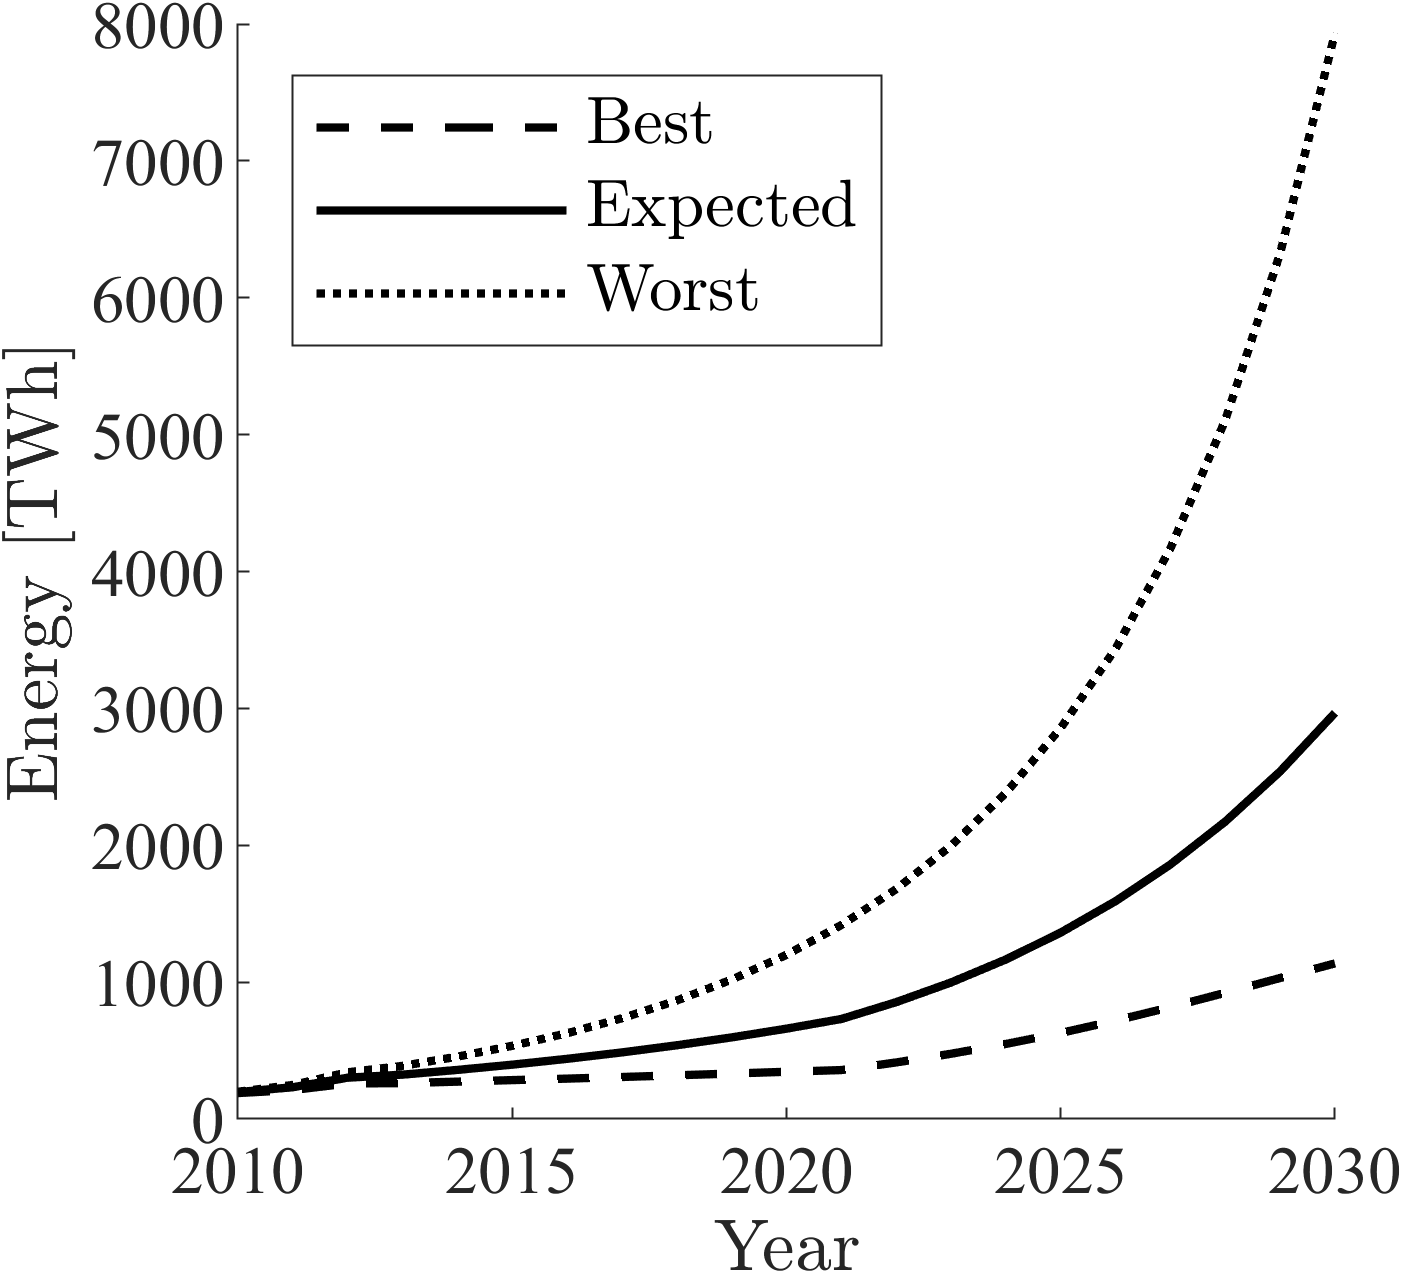
\includegraphics[width= \textwidth]{data_center_energy_consumption.png} \label{fig:dataCenterEnergy}
%	\end{subfigure}
%	\hfill
%	\begin{subfigure}[b]{0.30\textwidth}
%		\subcaption{}
%		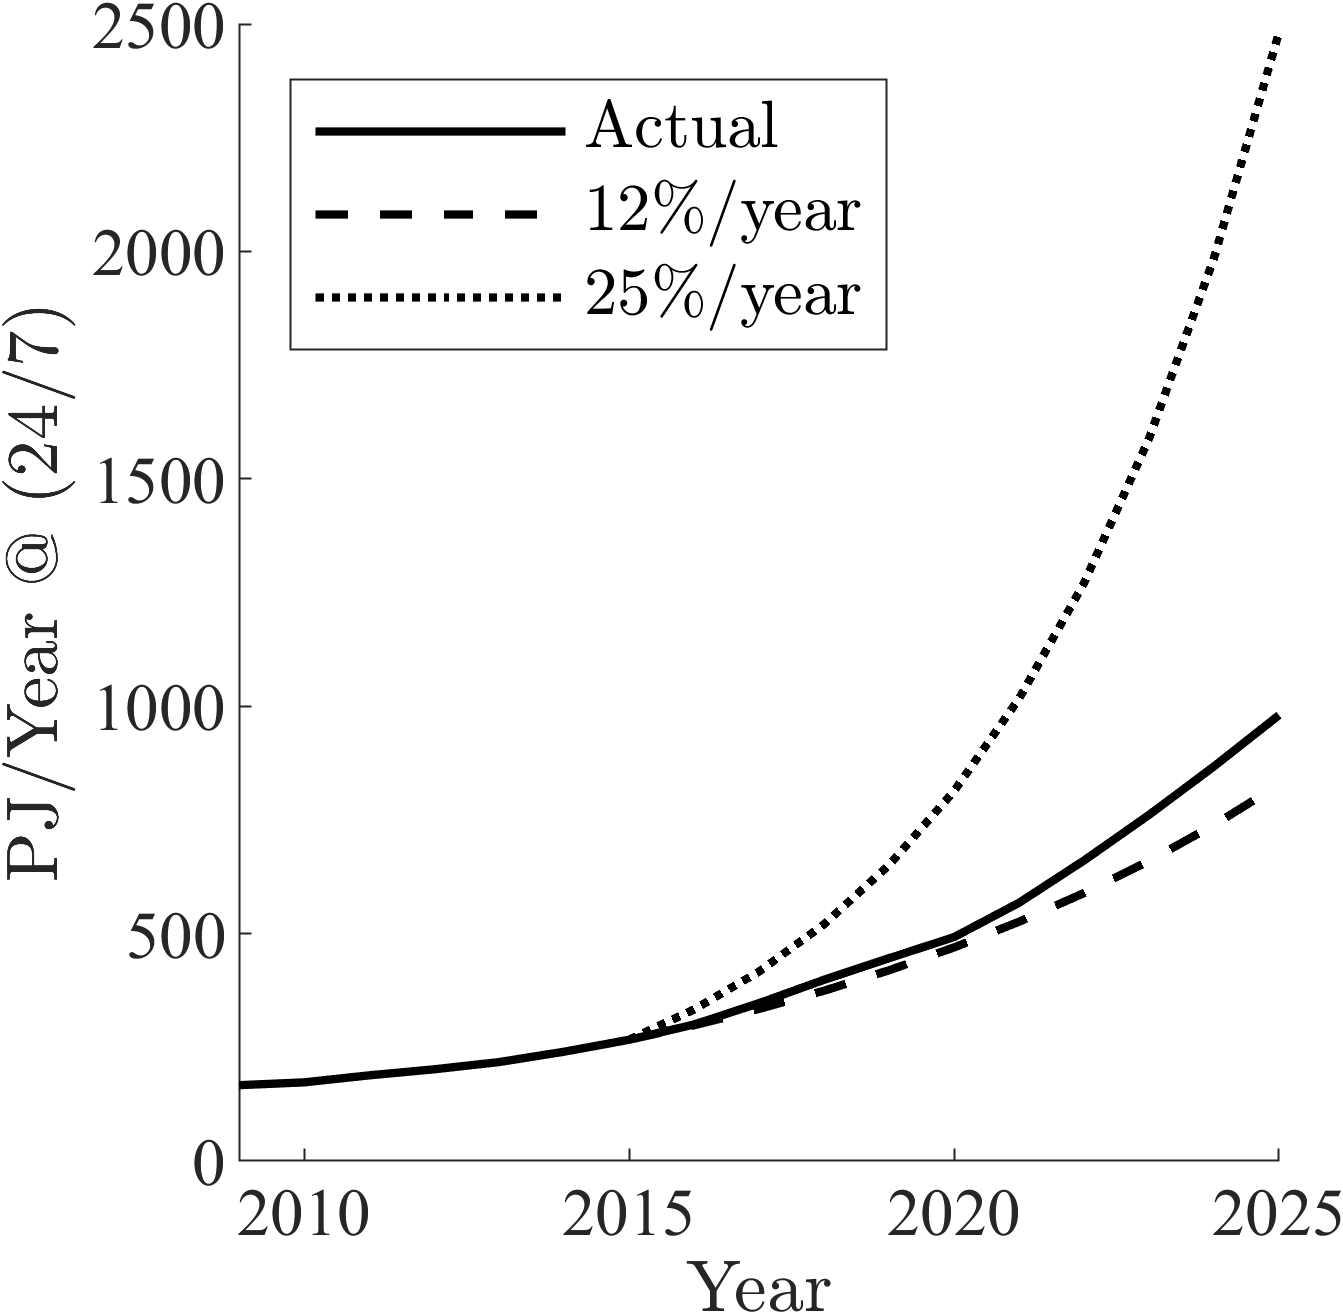
\includegraphics[width=\textwidth]{ir_energy_projections.png} \label{fig:ir_energy}
%	\end{subfigure}
%	\hfill
%	\begin{subfigure}[b]{0.30\textwidth}
%		\subcaption{}
%		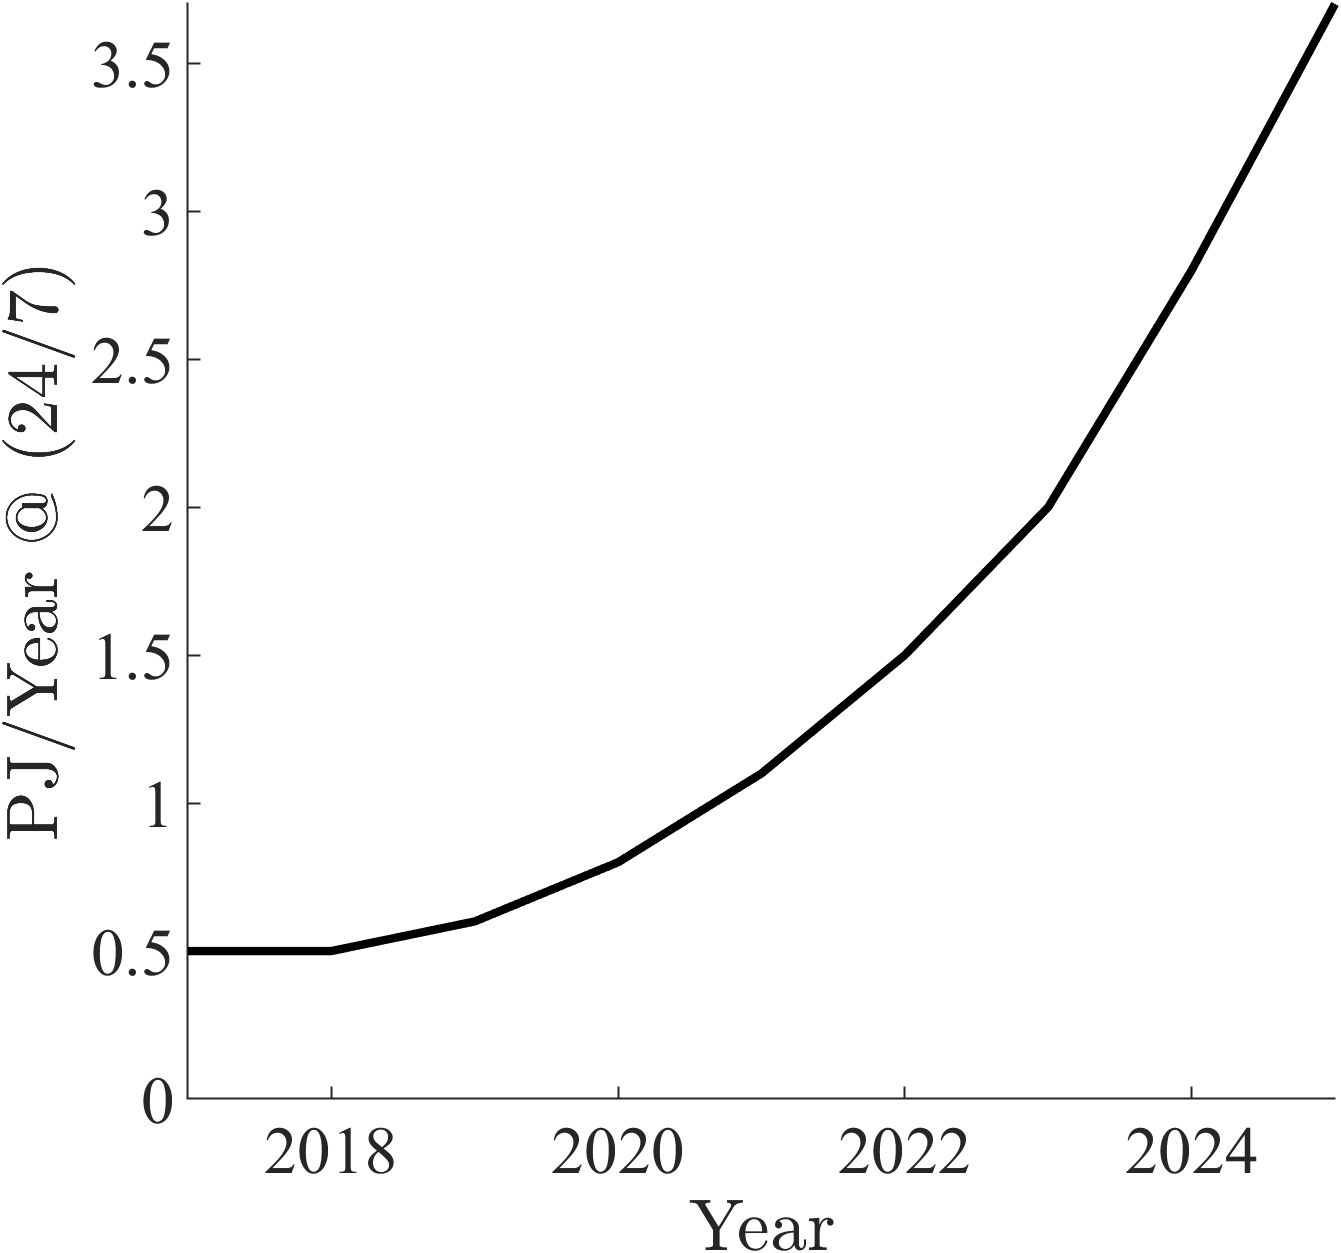
\includegraphics[width=\textwidth]{cb_energy_projections.png} \label{fig:cobot_energy}
%	\end{subfigure}	
%	\hspace*{\fill}
%	\caption[] {\label{fig:energy_demands_AI_robotics} \textbf{Energy demands in \ac{ai} and robotics.} (\subref{fig:dataCenterEnergy}) Global electricity demand of data centers, adapted from \cite{andrae2015global}. The estimated World Robot Energy Consumption of (\subref{fig:ir_energy}) industrial robots and (\subref{fig:cobot_energy}) collaborative robots.}
%\end{figure*}
%% ---


% ---
\begin{figure*}[t!]
	\centering
	\hspace*{\fill}
	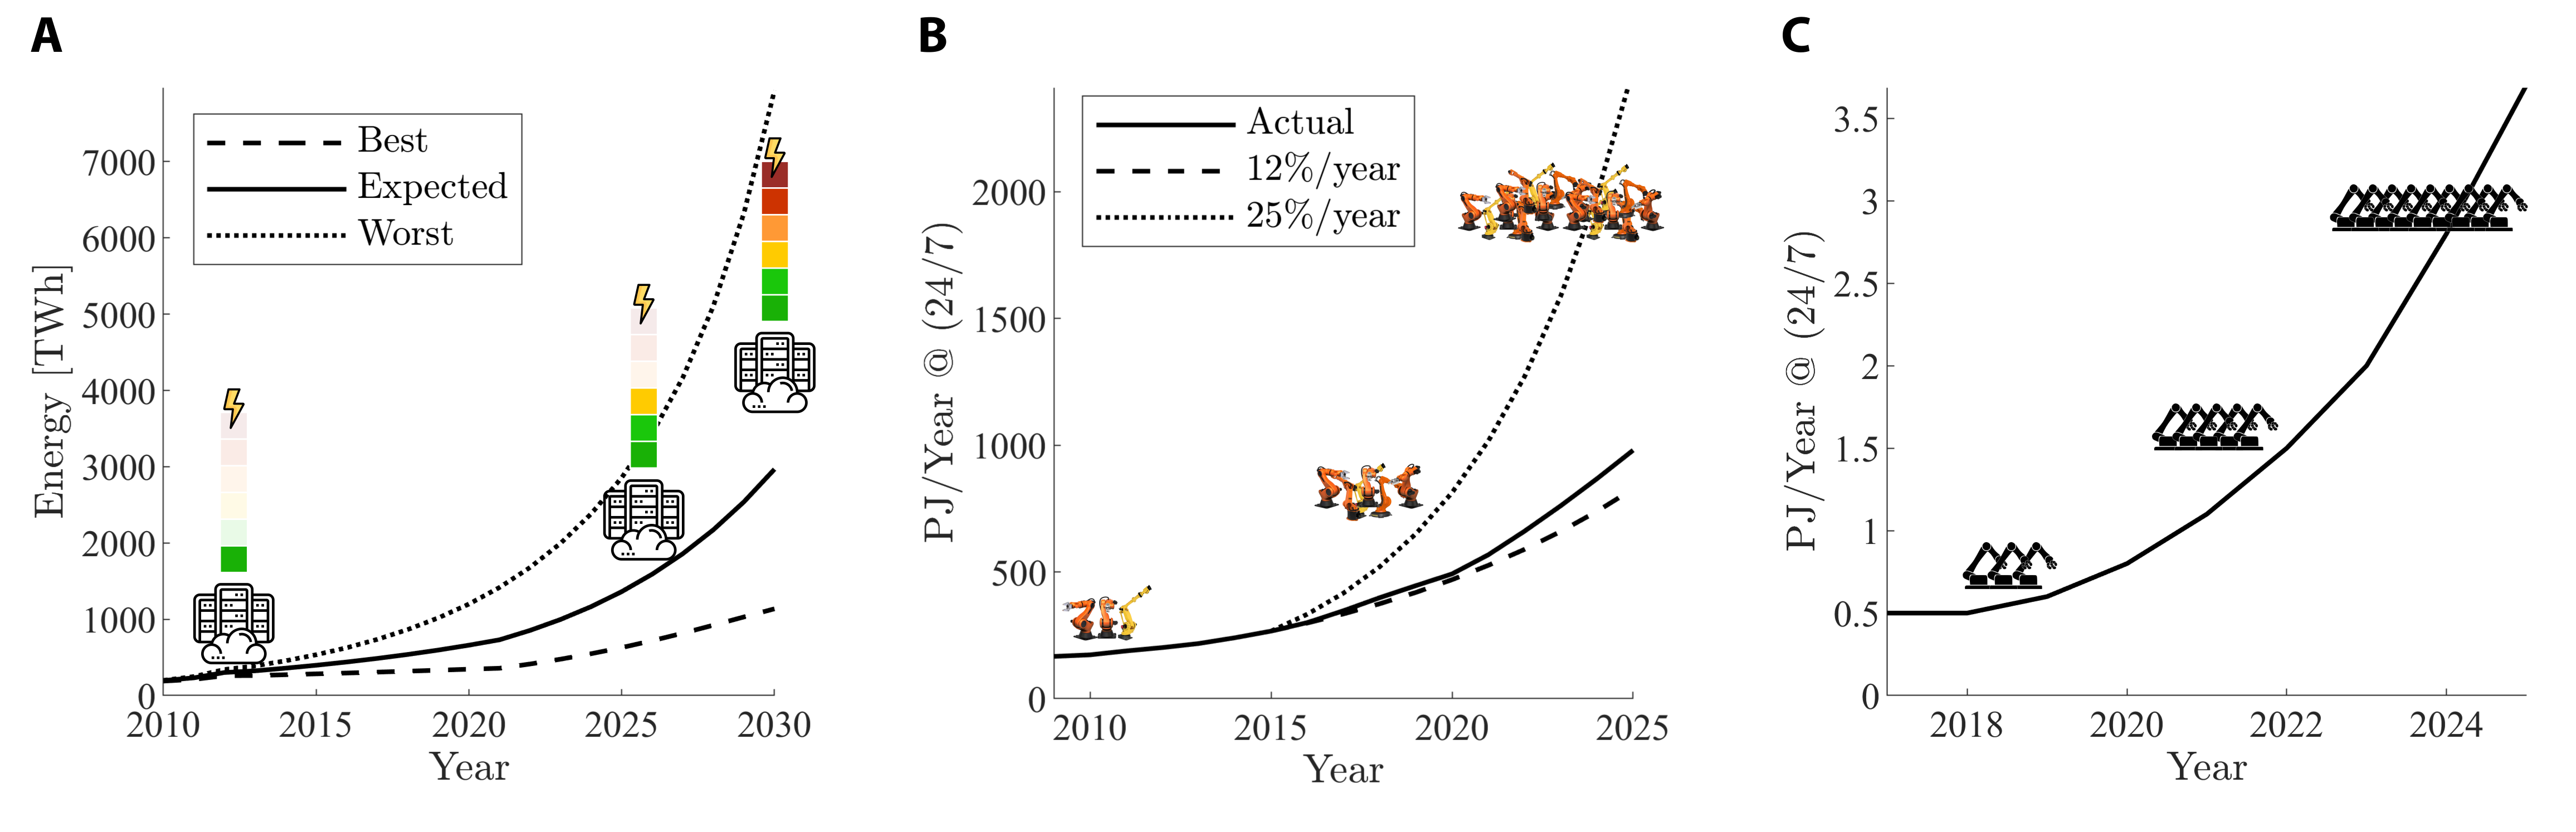
\includegraphics[width=\textwidth]{energy_consumption_trends_ai_and_robotics.png}
	\hspace*{\fill}
	\caption[] {\label{fig:energy_consumption_trends_ai_and_robotics} \textbf{Energy demands in \ac{ai} and robotics.} Global electricity demand of data centers (\textsc{Left}), adapted from \cite{andrae2015global}. The estimated World Robot Energy Consumption of industrial (\textsc{Middle}) and  collaborative robots (\textsc{Right}).}
\end{figure*}
% ---



Consider, for instance, the latest breakthroughs ushered in by generative \ac{ai}, including large language models (LLM) and text-to-image models. These models boast billions of parameters and necessitate thousands of deep learning \ac{gpu} units and millions of \ac{gpu} hours for training \cite{Vanian2023ChatGPTgenerativeAI, Corbyn2023Nvidiachipmaker}. As more \ac{ai} applications are developed, the demand for \ac{ai} infrastructure surges, leading to a substantial increase in \ac{gpu}-based \ac{ai} servers being sold to meet this demand. Naturally, this escalation in demand translates to a parallel rise in data center energy consumption. Globally, data center energy consumption surged from 200 TWh in 2015 to an estimated 220-320 TWh in 2021, according to data from the International Energy Agency \footnote{Data from the International Energy Agency, available at \url{https://www.iea.org/reports/data-centres-and-data-transmission-networks}}. This concerning trend is shown in~%Fig.~\ref{fig:dataCenterEnergy}.
Fig.~\ref{fig:energy_consumption_trends_ai_and_robotics} (\textsc{Left} panel)

\paragraph*{\textbf{Challenge 2} (C2): The escalating energy demand of a robotic revolution}\label{sec:robots_challenge}
The continuous growth in the number of robots in operation is a notable trend amplified by the rise of Industry 4.0 and the implementation of smart factories, alongside the expanding utilization of robots in various service-oriented applications. This rapid proliferation of robots has even been referred to as the \textit{cambrian explosion} of robotics \cite{Pratt2015Iscambrianexplosion}. Despite the advancements in robot technology that have yielded improved energy efficiency, the predominant focus remains on individual systems, often disregarding the aggregated impact of all active units.

Over more than an decade, the installation base of industrial robots has undergone a remarkable transformation. According to data from the International Federation of Robotics (IFR), this installation base escalated from 1.2 million units in 2012 to approximately 4.2 million units in 2023, an astonishing surge constituting a 350 \% increase with an average annual growth rate close to 12 \% \cite{IFR2024WorldRobotics2024}. Extrapolation of this trend suggests that in the coming years, six million robots will be operational within factories across the globe\footnote{These projections closely align with the slightly more cautious estimates presented by \textit{The Boston Consulting Group} in \cite{Sirkin2015HowRobotsWill}.}. Using the estimated install base and under the assumption of round-the-clock operation, we can approximate the forthcoming energy demand attributable to industrial robots---termed the \textit{World Robot Energy Consumption} (WREC), shown in~%Fig.~\ref{fig:ir_energy} 
Fig.~\ref{fig:energy_consumption_trends_ai_and_robotics} (\textsc{Middle} panel). To contextualize the significance of the WREC, in 2025, it constitutes 7.2 \% of Germany's installed electricity generation capacity \cite{FraunhoferISENetinstalledelectricity}. A description of how we arrived at these estimates is provided in Sec.~\ref{sec:app_robot_ener_consumption}.

The far-reaching influence of collaborative and service robots echoes the significance observed among their industrial counterparts. Collaborative robots (cobots), for instance, have undergone a paradigm shift, progressing from accounting for a mere 6 \% of the market in 2017 to constituting around one-quarter of annual installations \cite{tobe2015}, as illustrated in Fig.~\ref{fig:industrial_cobot_share}. Drawing from analogous assumptions applied to industrial robots,~%Fig.~\ref{fig:cobot_energy}
Fig.~\ref{fig:energy_consumption_trends_ai_and_robotics} (\textsc{Right} panel) depicts the projected growth trajectory of cobots and its associated energy consumption. Concurrently, the domain of service robots is experiencing an analogous surge. For instance, estimates project the that the service robotics market will reach 56 billion euros in 2025 \cite{statista_service_robots}. These robots find utility across various fields, including logistics, defense, public relations, medical applications, and beyond, underlining their alignment with the escalating trends observed among industrial and collaborative robots.

\paragraph*{\textbf{Challenge 3} (C3): Energy for manufacturing}
Another aspect that often escapes attention is the energetic expenditure associated with manufacturing the hardware required for AI and robotics. This energy demand entails two primary facets. First, it involves the energy outlay for procuring the materials for robot manufacturing and the associated computational hardware (e.g., processors, \ac{gpu}s, and \ac{ai} servers). Second, it pertains to the energy consumption intrinsic to the manufacturing process. Given the direct correlation between energy demand and the number of \ac{ai}-powered robots produced, an exponential rise in the latter directly corresponds to escalated energy consumption for their production. The assessment and formulation of strategies to address this aspect constitute the crux of this challenge. While an immediate solution may not be evident, and since substantial energy savings in raw material procurement may be impractical, significant potential lies in the recycling of electronic components of computer and robot hardware as a means of conserving energy\footnote{An example of such an endeavor is the international competition \textit{Robothon\textsuperscript{\textregistered} - The Grand Challenge}, see~\url{https://automatica-munich.com/en/munich-i/robothon/}.}.

%\paragraph*{\textbf{Aim and contribution}}
%\myhl{This work provides a perspective on the challenges linked to the energetic demand associated with implementing current learning paradigms from (disembodied) artificial intelligence on the anticipated exponential numbers of future robotic agents. Particularly, we stress that inefficient knowledge utilization exacerbates these challenges, resulting in a rapidly escalating energy demand. Our study favors adopting a learning strategy that explicitly leverages interconnection and knowledge sharing among intelligent robotic systems. Consequently, we propose collective learning as the optimal paradigm to facilitate faster and more efficient learning, thereby mitigating the energetic challenges in AI for physical systems. Specifically, we examine the ideal knowledge-sharing dynamics that a group of robots must exhibit to effectively realize the benefits of a collective learning strategy.}

%\noindent \rule{\textwidth}{5pt}
\paragraph*{Energy expenditure in \ac{eai}}
%% ---
%\begin{figure*}[t!]
%	\centering
%	\hspace*{\fill}
%	\begin{subfigure}[t]{0.45\textwidth}
%		\subcaption{}
%		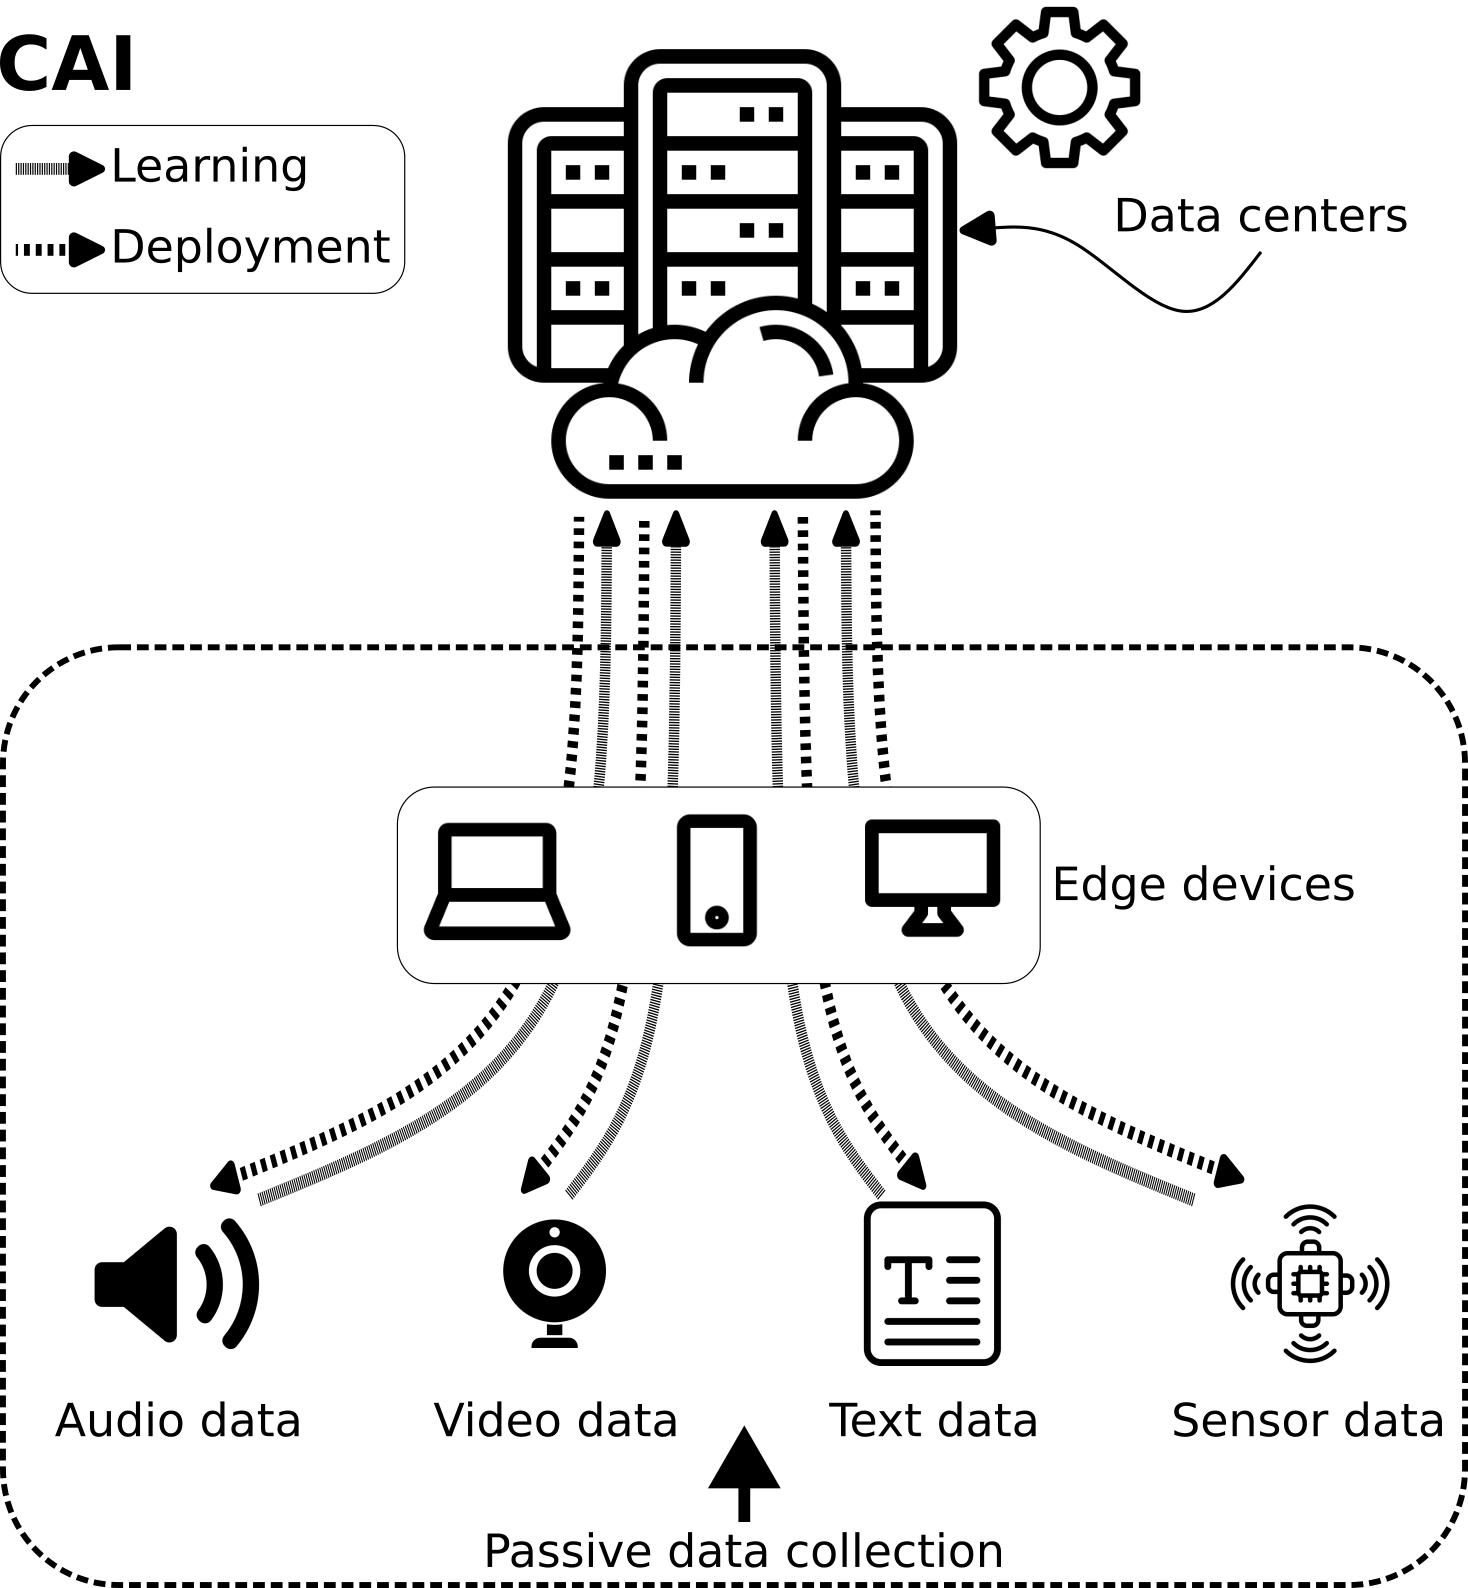
\includegraphics[width= \textwidth]{cai_concept.png} \label{fig:cai}
%	\end{subfigure}
%	\hfill
%	\begin{subfigure}[t]{0.45\textwidth}
%		\subcaption{}
%		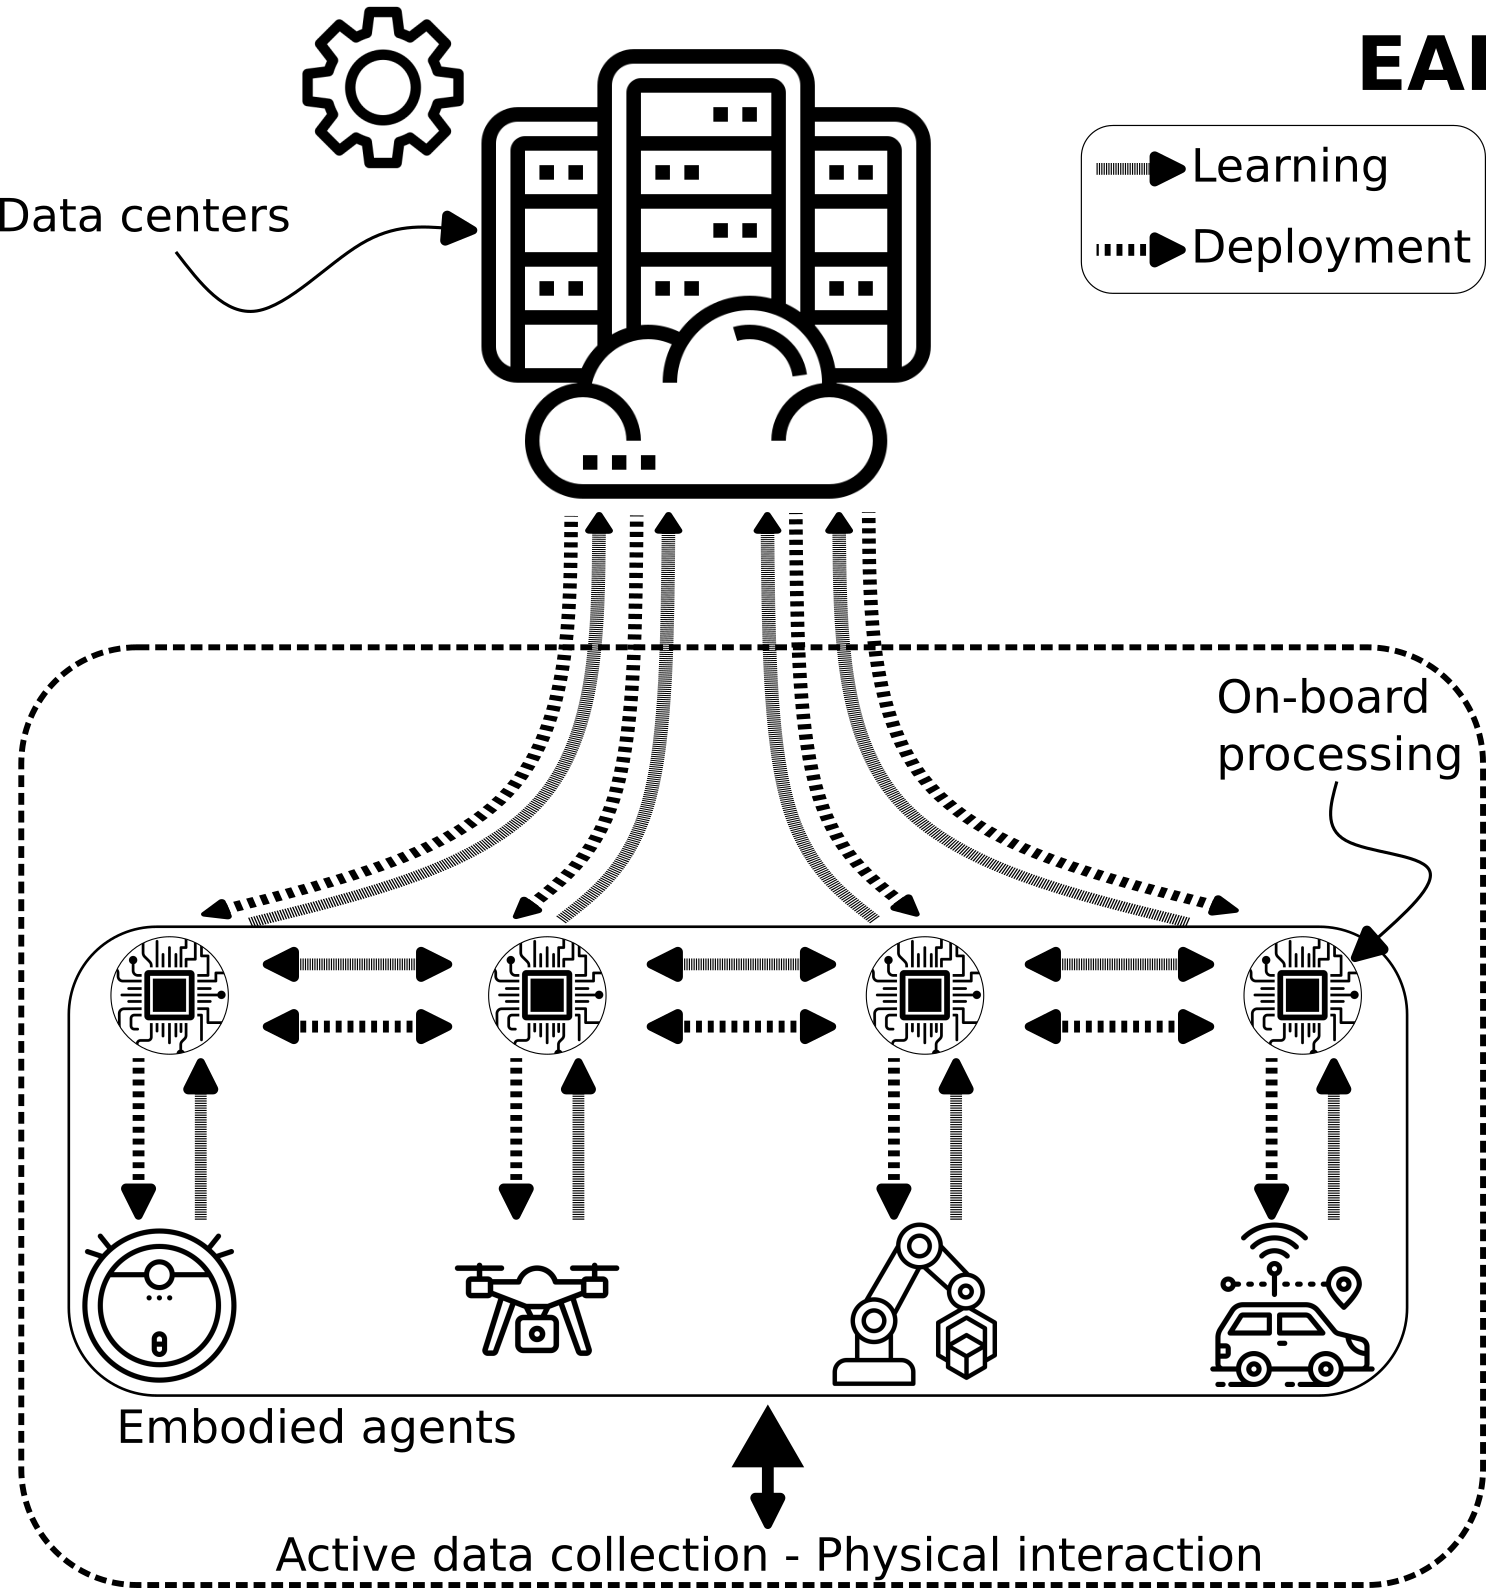
\includegraphics[width= \textwidth]{eai_concept.png} \label{fig:eai}
%	\end{subfigure}	
%	\hspace*{\fill}
%%	\\
%%	\hspace*{\fill}
%%	\begin{subfigure}[t]{0.95\textwidth}
%%		\subcaption{}
%%		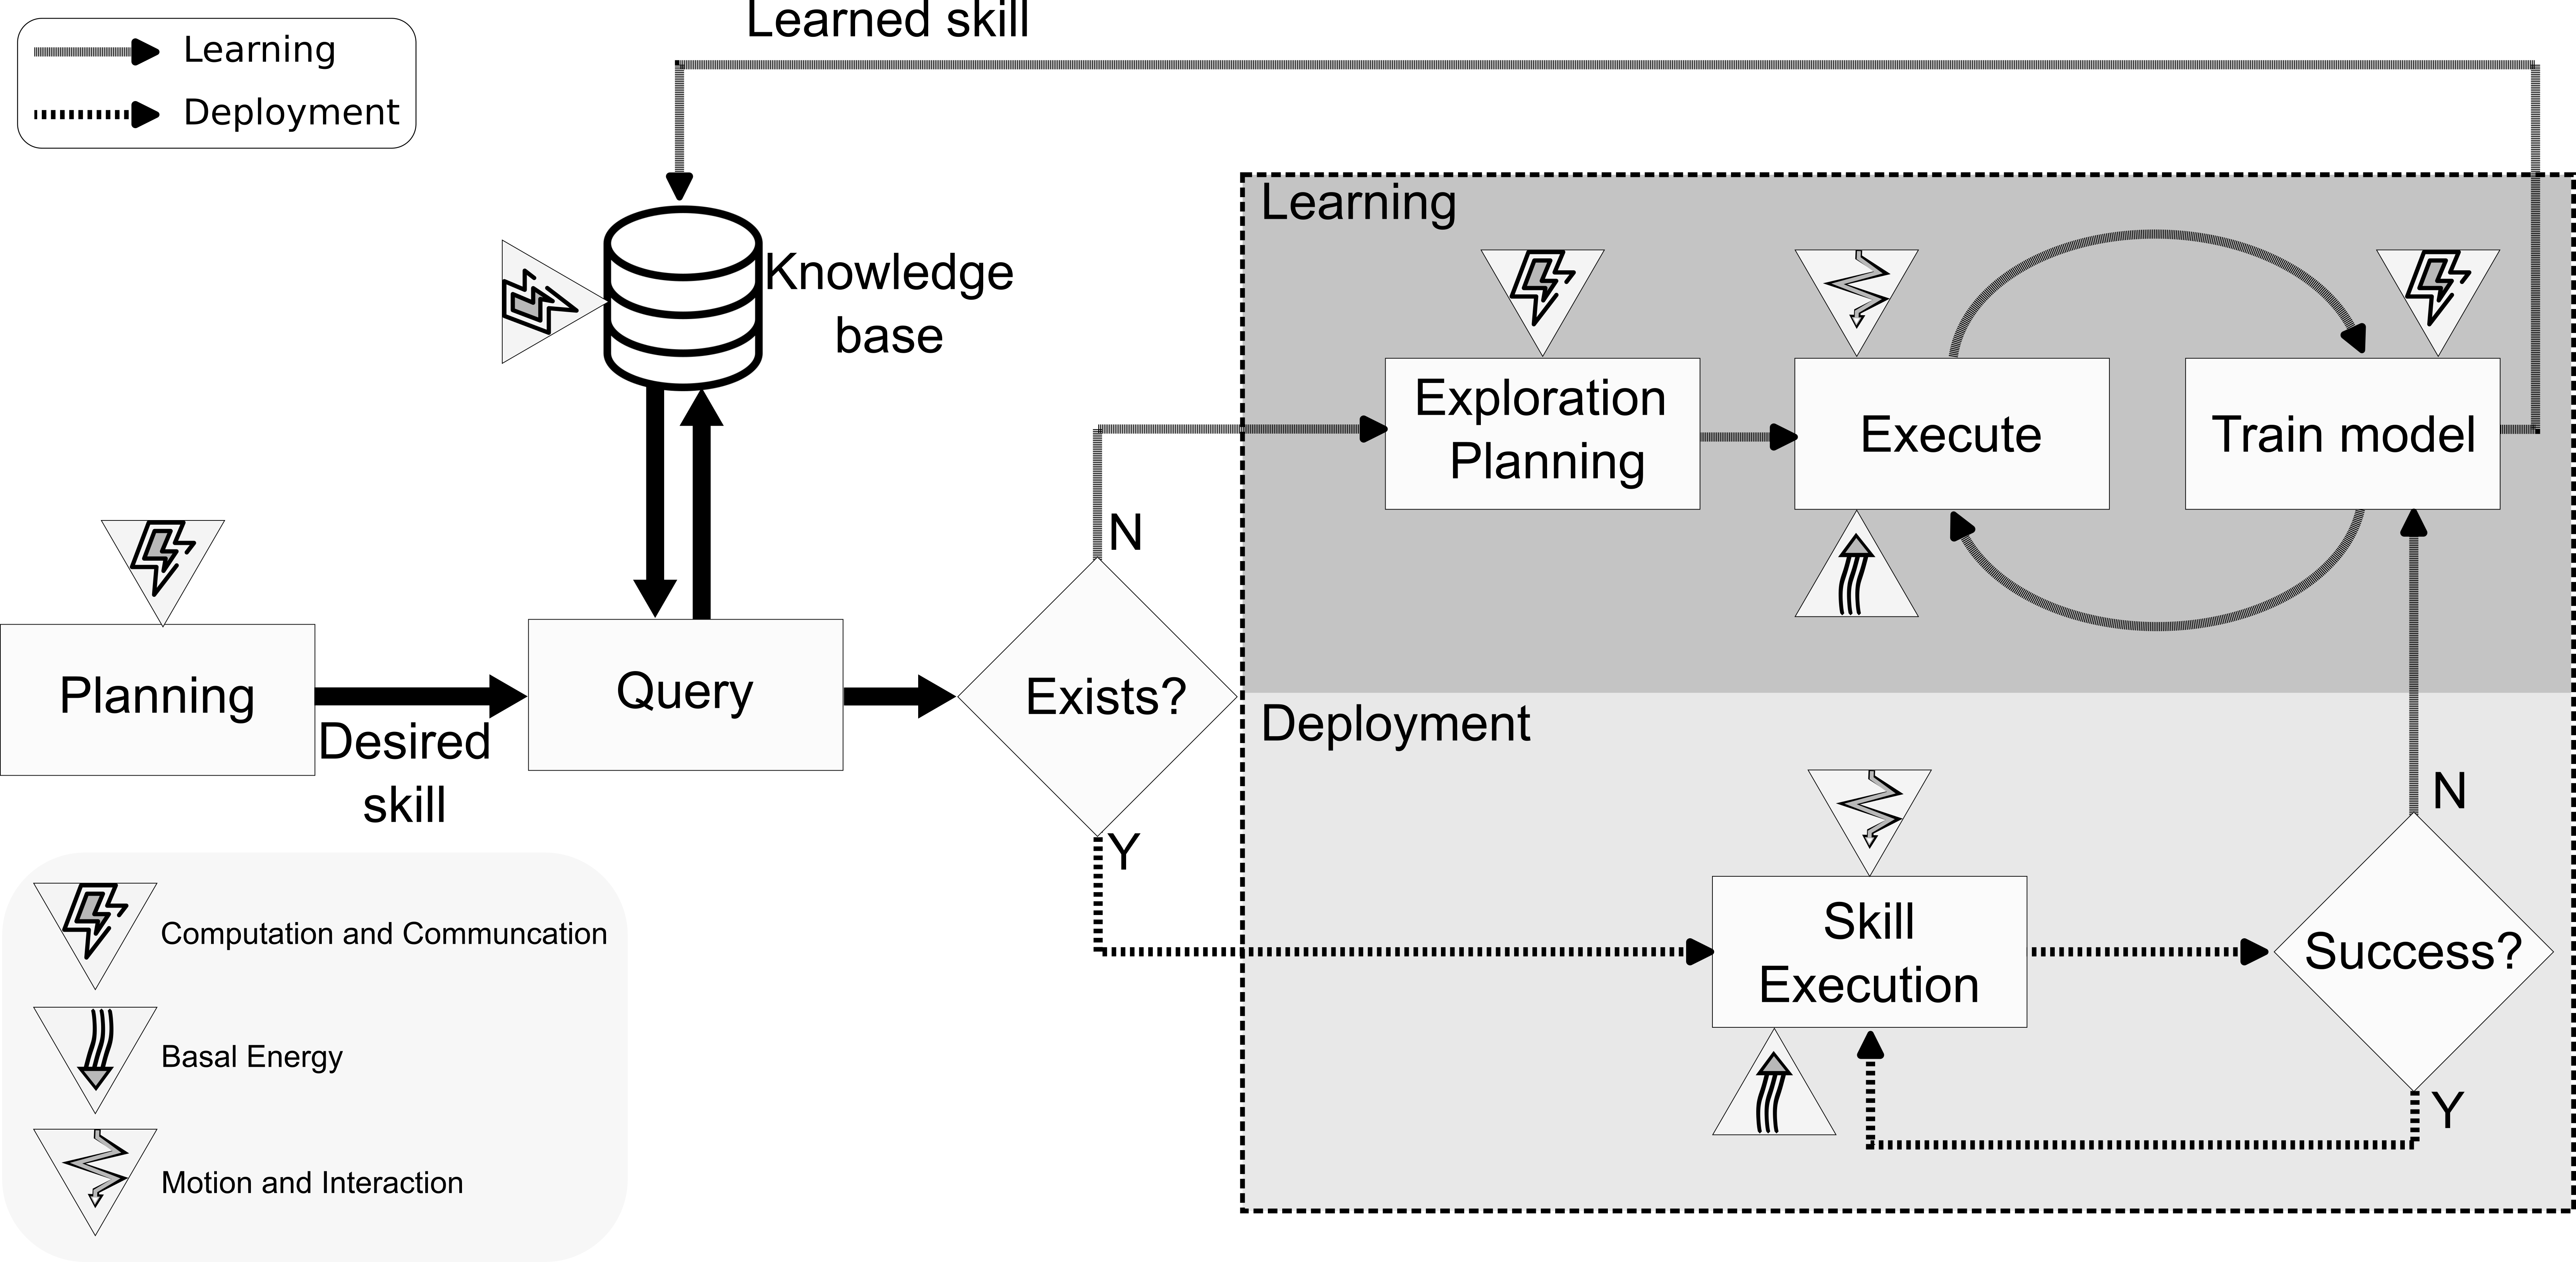
\includegraphics[width=\textwidth]{embodied_ai_learning_pipeline.png} \label{fig:embodied_ai_pipeline}
%%	\end{subfigure}	
%%	\hspace*{\fill}
%	\caption[] {\label{fig:cai_and_eai_general} \textbf{Classical and embodied AI.} Differences in learning and deployment in (\subref{fig:cai}) DAI and (\subref{fig:eai}) EAI. %(\subref{fig:embodied_ai_pipeline}) Standard skill execution pipeline of isolated EAI agents.
%	}
%\end{figure*}
%% ---

% ---
\begin{figure*}[t!]
	\centering
	\hspace*{\fill}
	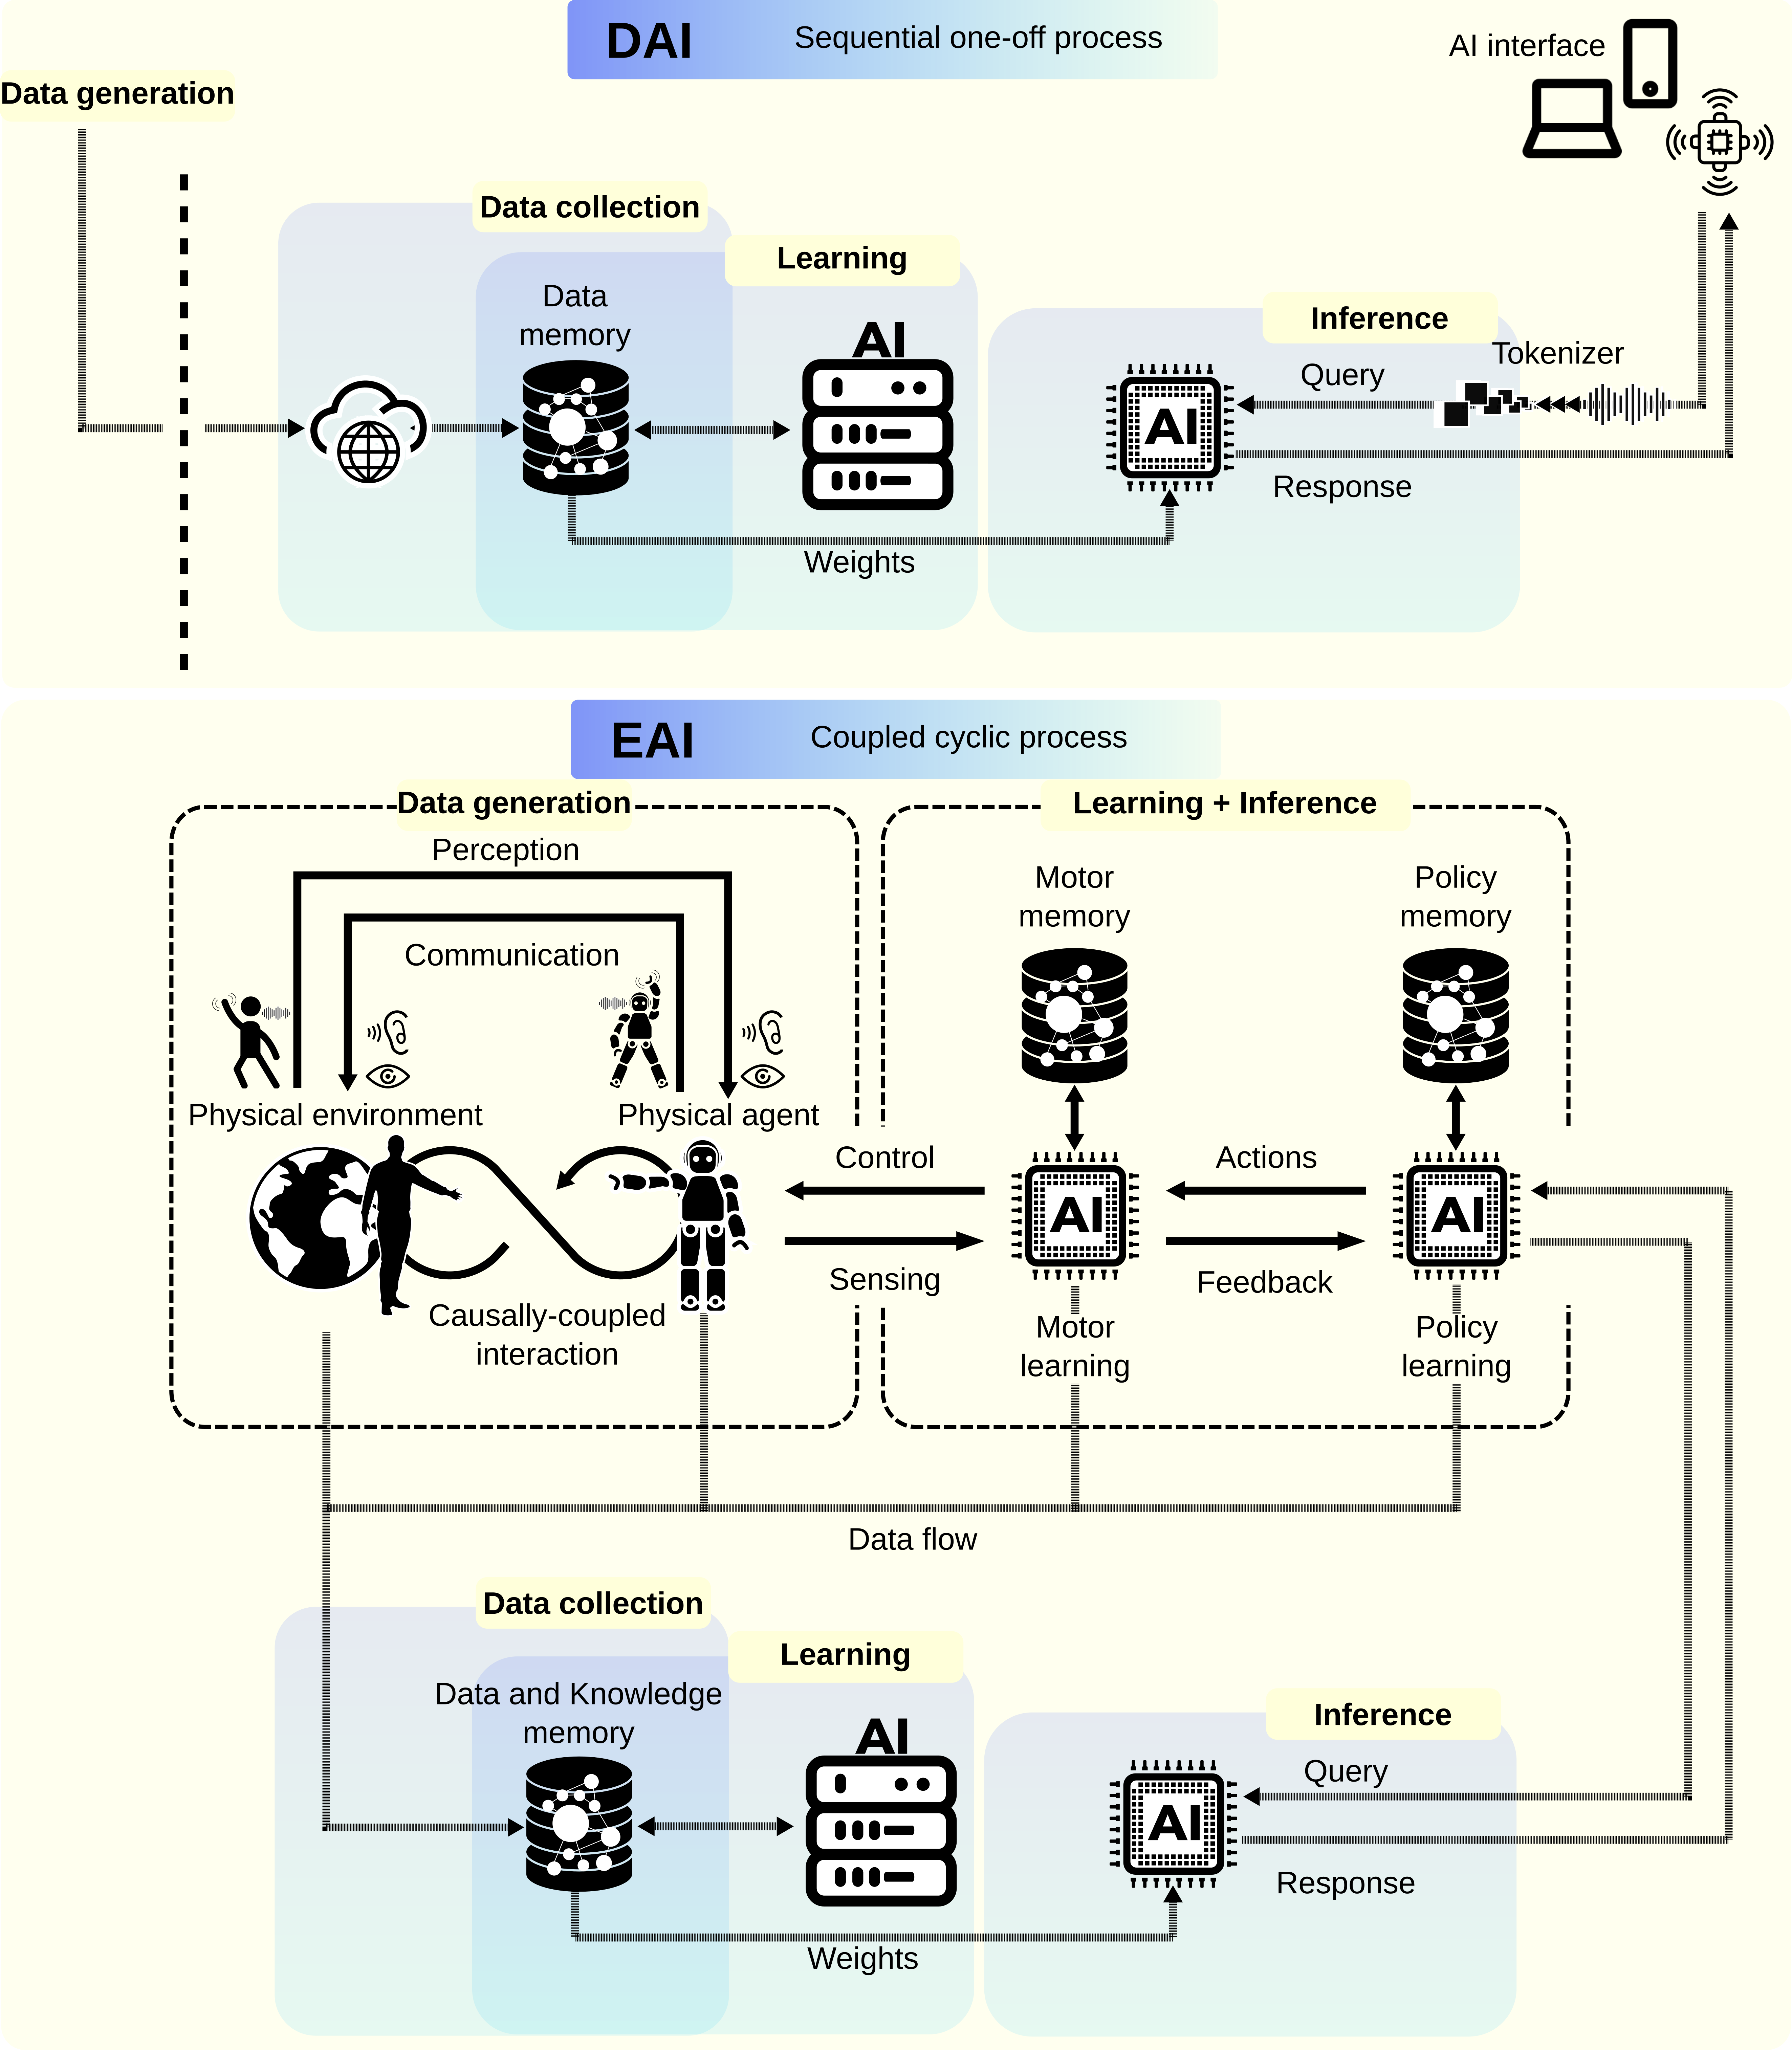
\includegraphics[width=0.95\textwidth]{eai_and_dai_concept_figure.png}
	\hspace*{\fill}
	\caption[] {\label{fig:eai_and_dai_concept_figure} \textbf{\Ac{dai} and \Ac{eai}.} Causally-coupled interaction of \ac{eai} agents with the enviroment generates data for learning. In \ac{dai}, data generation is a separate process.}
	
\end{figure*}
% ---


To address the energy demands of AI and robotics, we differentiate between classical \acl{dai} and \acl{eai}, as illustrated in Fig.~\ref{fig:eai_and_dai_concept_figure}. We consider \ac{dai} as the set of methods and algorithms that tackle purely computational problems, detached from embodied systems and lacking interaction with the physical world (see Fig.~\ref{fig:eai_and_dai_concept_figure}, \textsc{Bottom} panel). In \ac{dai}, data collection occurs passively through various edge devices, with a prototypical \ac{dai} agent not directly involved in generating or collecting training data. The energetic demands of \ac{dai} applications primarily stem from learning, i.e., training the models, and deployment, i.e., running inference and prediction \cite{Vries2023growingenergyfootprint}.

For \ac{dai} applications targeting diverse tasks or systems, successful knowledge transfer relies on the adequacy of the learning paradigm and both model and training data carrying enough information about the problem. However, in the absence of any of these factors, retraining, sometimes from scratch, becomes necessary, leading to highly energy-inefficient learning processes. Even if learning occurs only once, the ongoing deployment of the model can demand significant energy due to constant computationally intensive execution \cite{Vries2023growingenergyfootprint}. Thus, depending on the application, the energetic cost of learning and deployment in \ac{dai} can outweigh the benefits \cite{Strubell2019EnergyPolicyConsiderations}. This also applies to recent breakthroughs, such as transformer models for Natural Language Processing, whose results come accompanied by energetic challenges \cite{Cao2020TowardsAccurateReliable}.

The evolution towards \ac{eai}, the integration of \ac{ai} and robotics \cite{Pfeifer2004Embodiedartificialintelligence}, expands the energy usage spectrum. Unlike virtual environments, the real world cannot be faithfully replicated, despite considerable advances in sim-to-real applications \cite{Chebotar2019Closingsimreal}. Learning and deployment in \ac{eai} demand constant energy-expending interaction with the physical environment for active data generation, as depicted in the \textsc{Top} panel of Fig.~\ref{fig:eai_and_dai_concept_figure}, facilitated by physical agents like robots, vehicles, and drones. Mastering skills in the physical realm requires continuous and repeated execution, consuming energy for motion and interaction in each instance. Take autonomous driving, for example, where vehicles function as rudimentary \ac{eai} agents in structured human-made environments. Besides energy for autonomous movement, vehicles expend additional energy on motion to collect data necessary for retraining and improving the policy model. Another example is the usage of household robots to automate a high percentage of domestic chores \cite{Lehdonvirta2022futuresunpaidwork}. Such robots will undergo constant retraining due to the subtle and changing dynamics of household environments.
%% ---
%\begin{figure*}[t!]
%	\centering
%	\hspace*{\fill}
%	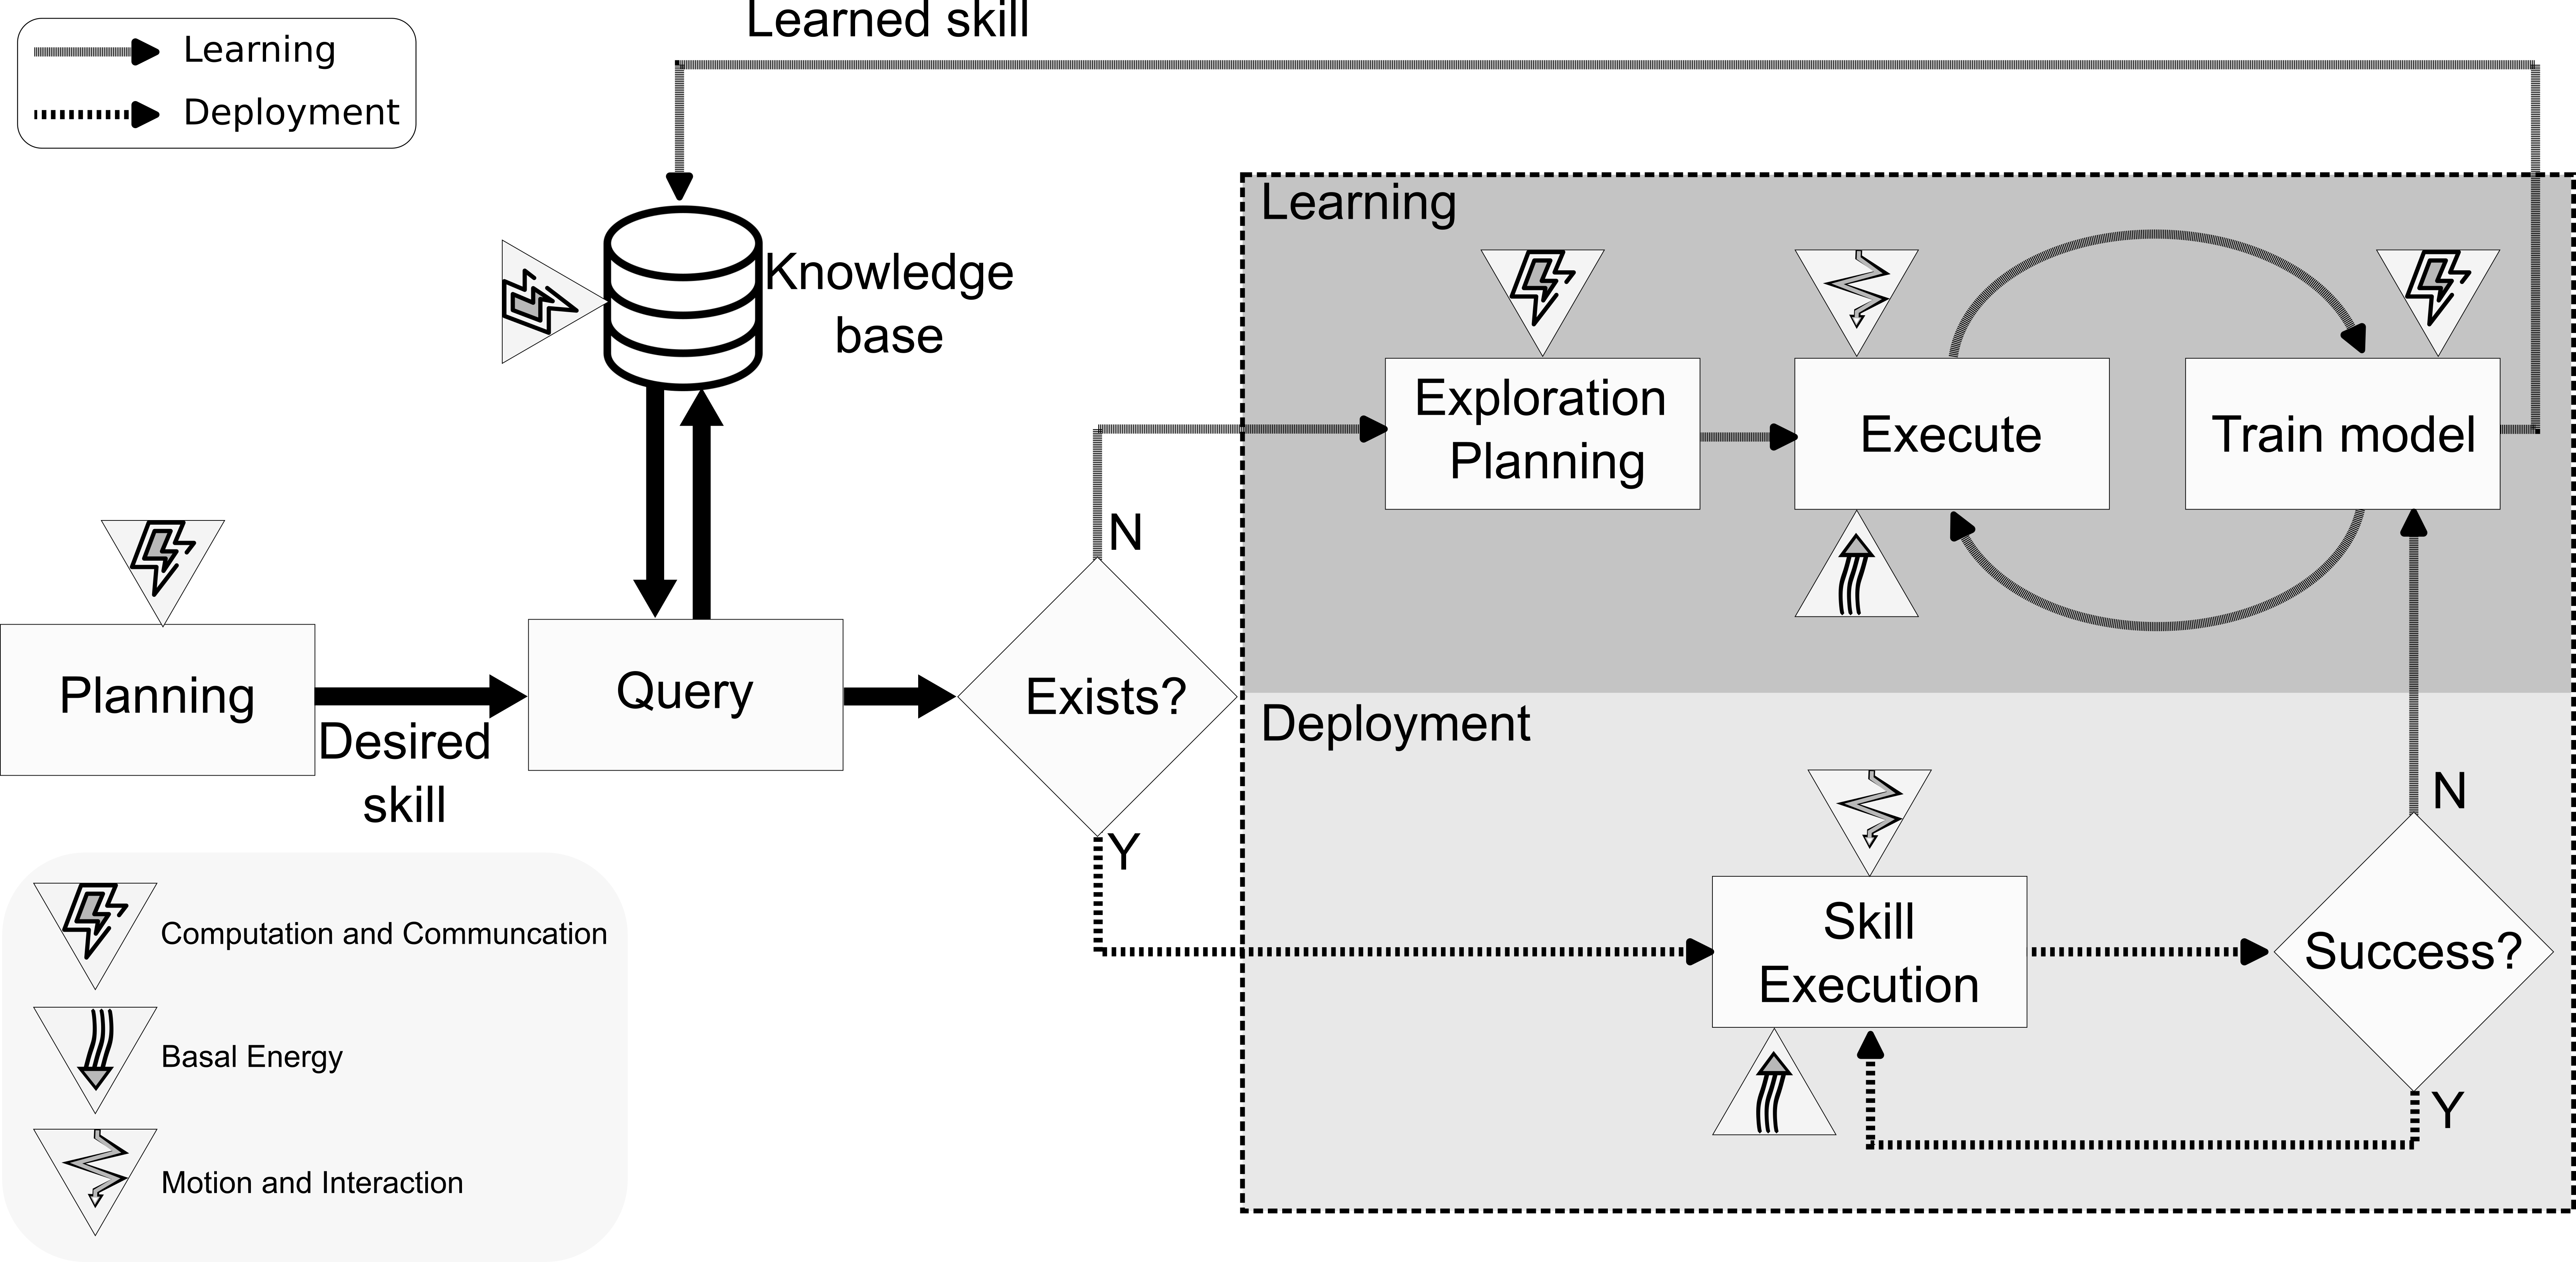
\includegraphics[width=0.95\textwidth]{embodied_ai_learning_pipeline.png}
%	\hspace*{\fill}
%	\caption[] {\label{fig:embodied_ai_pipeline} \textbf{Standard skill execution pipeline of a prototypical \ac{eai} agents.} {Three fundamental energy expenditure categories are identified during the learning or execution of a skill by an \ac{eai} agent.}}
%\end{figure*}
%% ---


% ---
\begin{figure*}[t!]
	\centering
	\hspace*{\fill}
	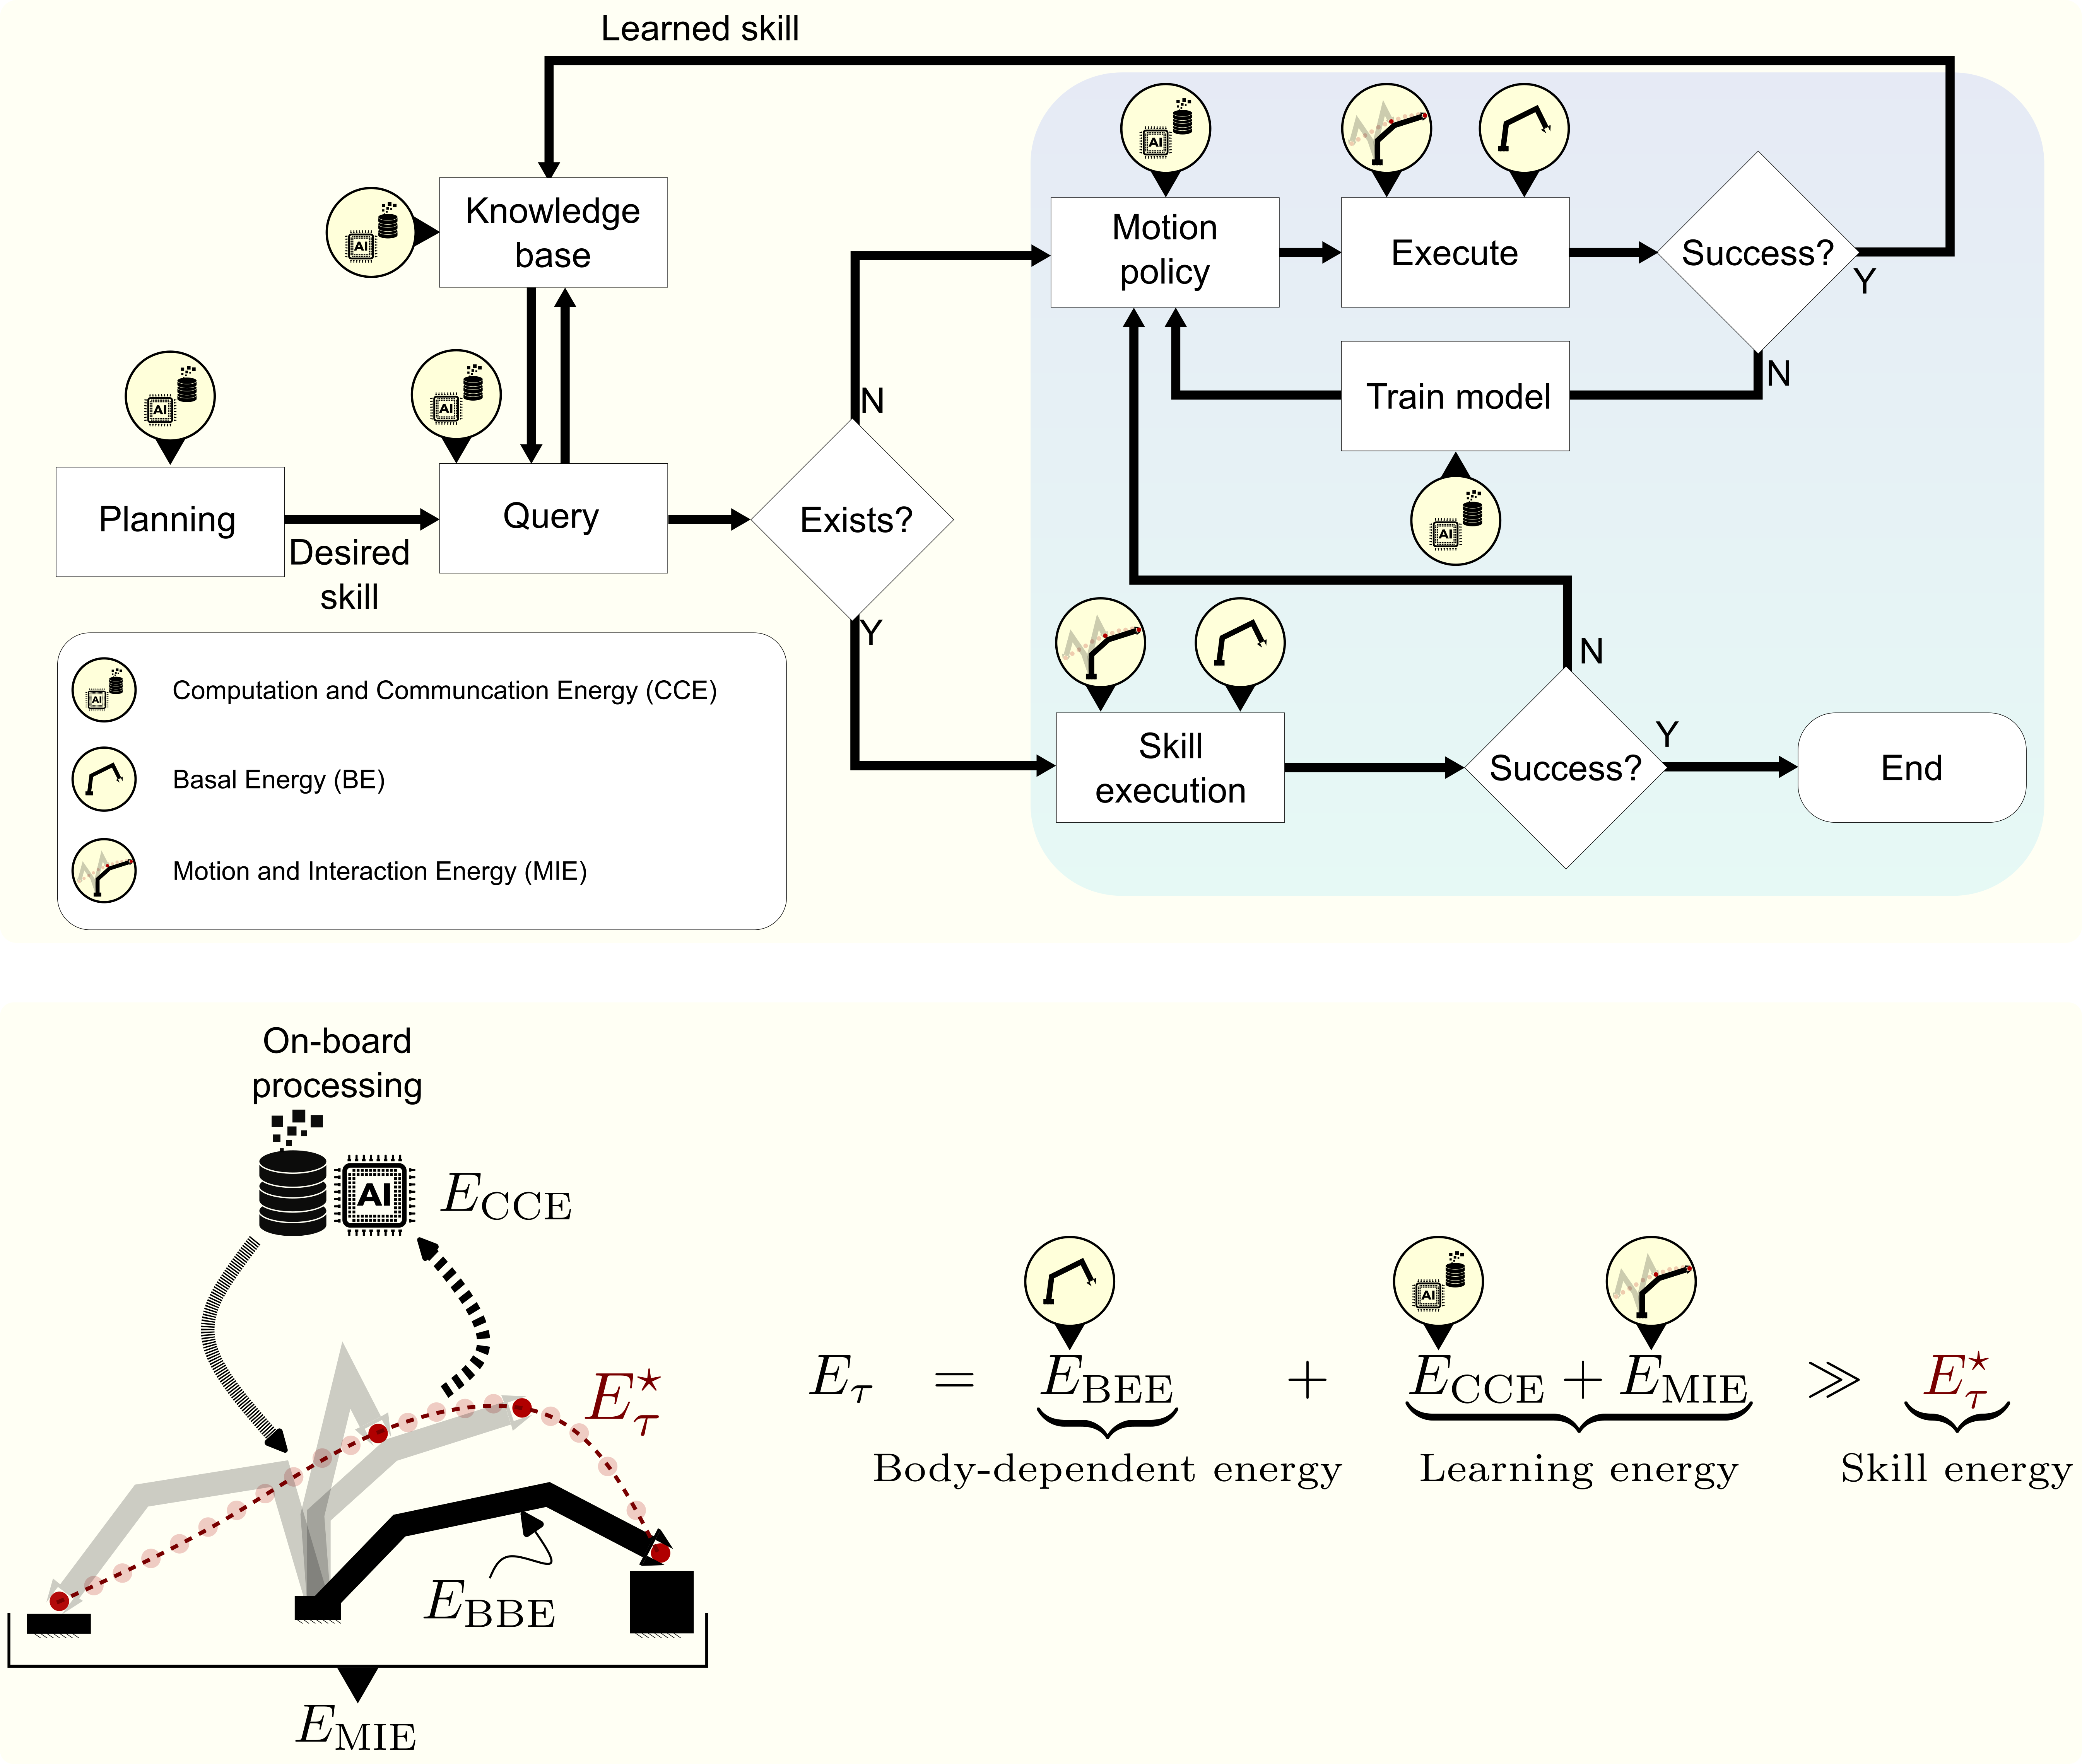
\includegraphics[width=0.95\textwidth]{eai_energy_categories.png}
	\hspace*{\fill}
	\caption[] {\label{fig:embodied_ai_pipeline} \textbf{Standard skill execution pipeline of a prototypical \ac{eai} agent.} {Three fundamental energy expenditure categories are identified during the learning or execution of a skill by an \ac{eai} agent.}}
\end{figure*}
% ---

Unlike the standard energy for learning and deployment classification in \ac{dai}, the analysis of the energetic requirements in \ac{eai} requires a different perspective. A closer look at the standard skill execution pipeline of a prototypical \ac{eai} agent ---Fig.~\ref{fig:embodied_ai_pipeline}---allows the identification of essential energetic expenditure categories, namely:
% ---
\begin{enumerate}
	\item \Ac{cce}: Coincident with \ac{dai}, it refers to the energy used by the computation and communication processes required by planning, querying, exploration, and training routines.
	\item \Ac{bee}: This body-related energy is associated with the execution of basic functions of the \ac{eai} agent. For example, operating energy, gravity compensation, and proprioceptive intelligence algorithms in robots, hovering in drones, running on-board system standby in autonomous vehicles, etc.
	\item \Ac{mie}: Defines the energy expended on physical interactions, namely, executing a particular skill in a certain form. For example, taking an object from an initial to a target location within a given time following a particular trajectory.
\end{enumerate}
% ---

An important fact in \ac{eai} is the existence of a lower bound on the energy required to carry out a skill that is independent of the agent. Consider a generic skill $\tau$---such as a pick-and-place operation---and suppose the optimal trajectory $p^\star$ for moving an object from its origin to its destination is known. The intrinsic properties of the object and the optimal trajectory $p^\star$ uniquely define the minimum energy requirement $E^\star_{\tau}$ needed to perform skill $\tau$. The implication is that the total energy expended by any agent in the process of mastering or executing a skill is higher than $E^\star_{\tau}$ as a result of the required computational ($E_\text{CCE}$), body-related ($E_\text{BEE}$), and physical interaction ($E_\text{MIE}$) energy expenditures; i.e.,
% ---
\begin{equation}\label{eq:skill_energy_in_eai}
	E_{\tau} =  \underbrace{E_\text{BEE}}_{\text{Body-dependent energy}} + \underbrace{E_\text{CCE} + E_\text{MIE}}_{\text{Learning energy}} \gg \underbrace{E^\star_{\tau}}_{\text{Skill energy}} .
\end{equation}
% ---
It is worth mentioning that if Eq.~\eqref{eq:skill_energy_in_eai} was used to describe the energy consumption of a task in \ac{dai}, $E_\text{BEE}$ could be associated with the edge devices and $E_\text{CCE}$ would represent the primary source of energy consumption. Additionally, the expenditures $E^\star_{\tau}$ and $E_\text{MIE}$ do not exist in \ac{dai} since physical interaction is absent.

%\paragraph*{\textbf{Aim and contribution}}
%This work provides a perspective on the challenges linked to the energetic demand associated with implementing current learning paradigms from (disembodied) artificial intelligence on the anticipated exponential numbers of future robotic agents. Particularly, we stress that inefficient knowledge utilization exacerbates these challenges, resulting in a rapidly escalating energy demand. Our study favors adopting a learning strategy that explicitly leverages interconnection and knowledge sharing among intelligent robotic systems. Consequently, we propose collective learning as the optimal paradigm to facilitate faster and more efficient learning, thereby mitigating the energetic challenges in AI for physical systems. Specifically, we examine the ideal knowledge-sharing dynamics that a group of robots must exhibit to effectively realize the benefits of a collective learning strategy.

% ===================================================================================================
\paragraph*{\textbf{Problem statement}}
The rapid proliferation of robotic agents, driven by advances in artificial intelligence (AI) and machine learning, poses a critical challenge: the escalating energy demand associated with current learning paradigms. Traditional \ac{ai} learning strategies, designed primarily for disembodied systems, fail to leverage knowledge utilization in large-scale robotic deployments. This inefficiency exacerbates energy consumption, particularly as robots increasingly rely on interaction-intensive learning and adaptation processes.

A fundamental question arises:
% ---
\begin{tcolorbox}
%	\begin{assumption}\label{question:research_question}
		How can robotic systems learn efficiently while minimizing energy costs?
%	\end{assumption}
\end{tcolorbox}
% ---
\noindent To address this, we argue that a paradigm shift is necessary---one that explicitly leverages interconnection and knowledge sharing among intelligent robotic systems. \Ac{cl} emerges as a promising solution, enabling robots to acquire and disseminate skills more efficiently, thus reducing redundant computations and overall energy consumption. This work explores the optimal knowledge-sharing dynamics required for a group of robots to fully realize the benefits of collective learning, paving the way for more sustainable \ac{ai}-driven robotics.


% ===================================================================================================
%                                                 |                                                 |
%                                                 |                                                 |
% -------------------------------------------- SECTION ---------------------------------------------|
%                                                 |                                                 |
%                                                 |                                                 |
% ===================================================================================================
\section*{Related works}
The trends depicted in~%Fig.~\ref{fig:energy_demands_AI_robotics}
Fig.~\ref{fig:energy_consumption_trends_ai_and_robotics} suggest that the energy expenditures for computation and communication, basal functions, and motion and interaction will likely follow a similar pattern. The implication is straightforward: as the number of \acl{ai} applications and robotic systems increases, so does their associated energy demand. Consequently, the energy requirements of \acl{dai} and \acl{eai} have recently received significant attention within the \acl{ai} and robotics research communities.

The escalating energy consumption of \acl{ai}, particularly of machine learning, has raised concerns about its adverse environmental impact. Most research in this area focuses on the computational and infrastructural requirements for training and running modern learning algorithms---such analyses directly correlate with the computational and communication energy expenditure. Recent works on this matter have delved into the efficiency of computation-intensive deep learning algorithms \cite{Schwartz2019GreenAI,Vinuesa2020roleartificialintelligence,Strubell2019EnergyPolicyConsiderations,Luccioni2023EstimatingCarbonFootprint}. In parallel, various metrics have been established to gauge the energy consumption of machine learning algorithms. These include assessing energy efficiency during development phases \cite{Zhou2020HULKEnergyEfficiency}, analyzing accuracy, model size, time, and CPU/\ac{gpu} energy consumption for training and inference phases \cite{Dalgren2019GreenMLmethodology}, as well as encompassing other system-level performance indicators like real-time metrics, instruction-level analysis, and hardware-level power estimation \cite{GarciaMartin2019Estimationenergyconsumption}. Recent works on large language models have discussed various aspects such as hardware efficiency, model architectures, and algorithms in relation to energy consumption \cite{Vries2023growingenergyfootprint} and provide comparisons including their power consumption and CO$_2$ emissions \cite{SIHCAI2023ArtificialIntelligenceIndex}.

Despite growing awareness of \ac{ai}'s energy consumption, tangible actions to address underlying issues and propose remedies remain scarce and predominantly focus on \ac{dai} applications. Yet, it is crucial to recognize the challenges posed by \ac{eai} systems. Unlike state-of-the-art machine learning models (e.g., transformer models) that are mostly trained once on a large amount of data, \ac{eai} agents have a constant need for energy-consuming retraining and evaluation processes. From the \ac{eai} perspective, ongoing efforts to minimize \ac{bee} and improve the \ac{mie} advocate strategies such as elastic actuation and optimized hardware selection and storage, energy sharing, and motion planning \cite{CUT2015Smoothrobotmovements, Mohammed2014MinimizingEnergyConsumption, Chemnitz2011Analyzingenergyconsumption,Vasarhelyi2023OverviewEnergiesProblems,Sekala2024SelectedIssuesMethods}.

As for \ac{cce}, it is essential to design better hardware for more efficient parallel computing and to decentralize the computation, leveraging the local processing capabilities of edge devices and robots. These capabilities have been highlighted in concepts such as the Internet of Robotic Things \cite{Vermesan2020InternetRoboticThings,Sekala2024SelectedIssuesMethods}. Perhaps even more relevant is to define sample-efficient algorithms with optimized models that account for the recurrent learning, inference, and prediction processes in \ac{eai} agents. We believe that achieving greater energy efficiency in AI requires a broader perspective than just enhancing hardware and optimizing the individual agents' learning strategies. The actual key to a significant breakthrough lies in tapping into the vast reservoir of knowledge accumulated by \ac{eai} systems.

Persistently using learning paradigms that fail to actively encourage and systematically utilize knowledge exchange among agents has a detrimental effect on energy consumption. Promoting and leveraging concurrent knowledge exchange can alleviate the burdens associated with the \ac{cce} and \ac{mie} expenditures in \ac{eai} since it can reduce the computational and mechanical energy required to acquire new skills. To explore this uncharted terrain, we propose considering the \ac{cl} paradigm introduced in \cite{Haddadin2014SystemzumErstellen,Haddadin2015Systemgeneratingsets} as a means to harness scalability and facilitate knowledge exchange, thereby enhancing energy efficiency in the domain of \acl{eai}.
% ---
\begin{figure*}[t!]
	\centering
	\hspace*{\fill}
	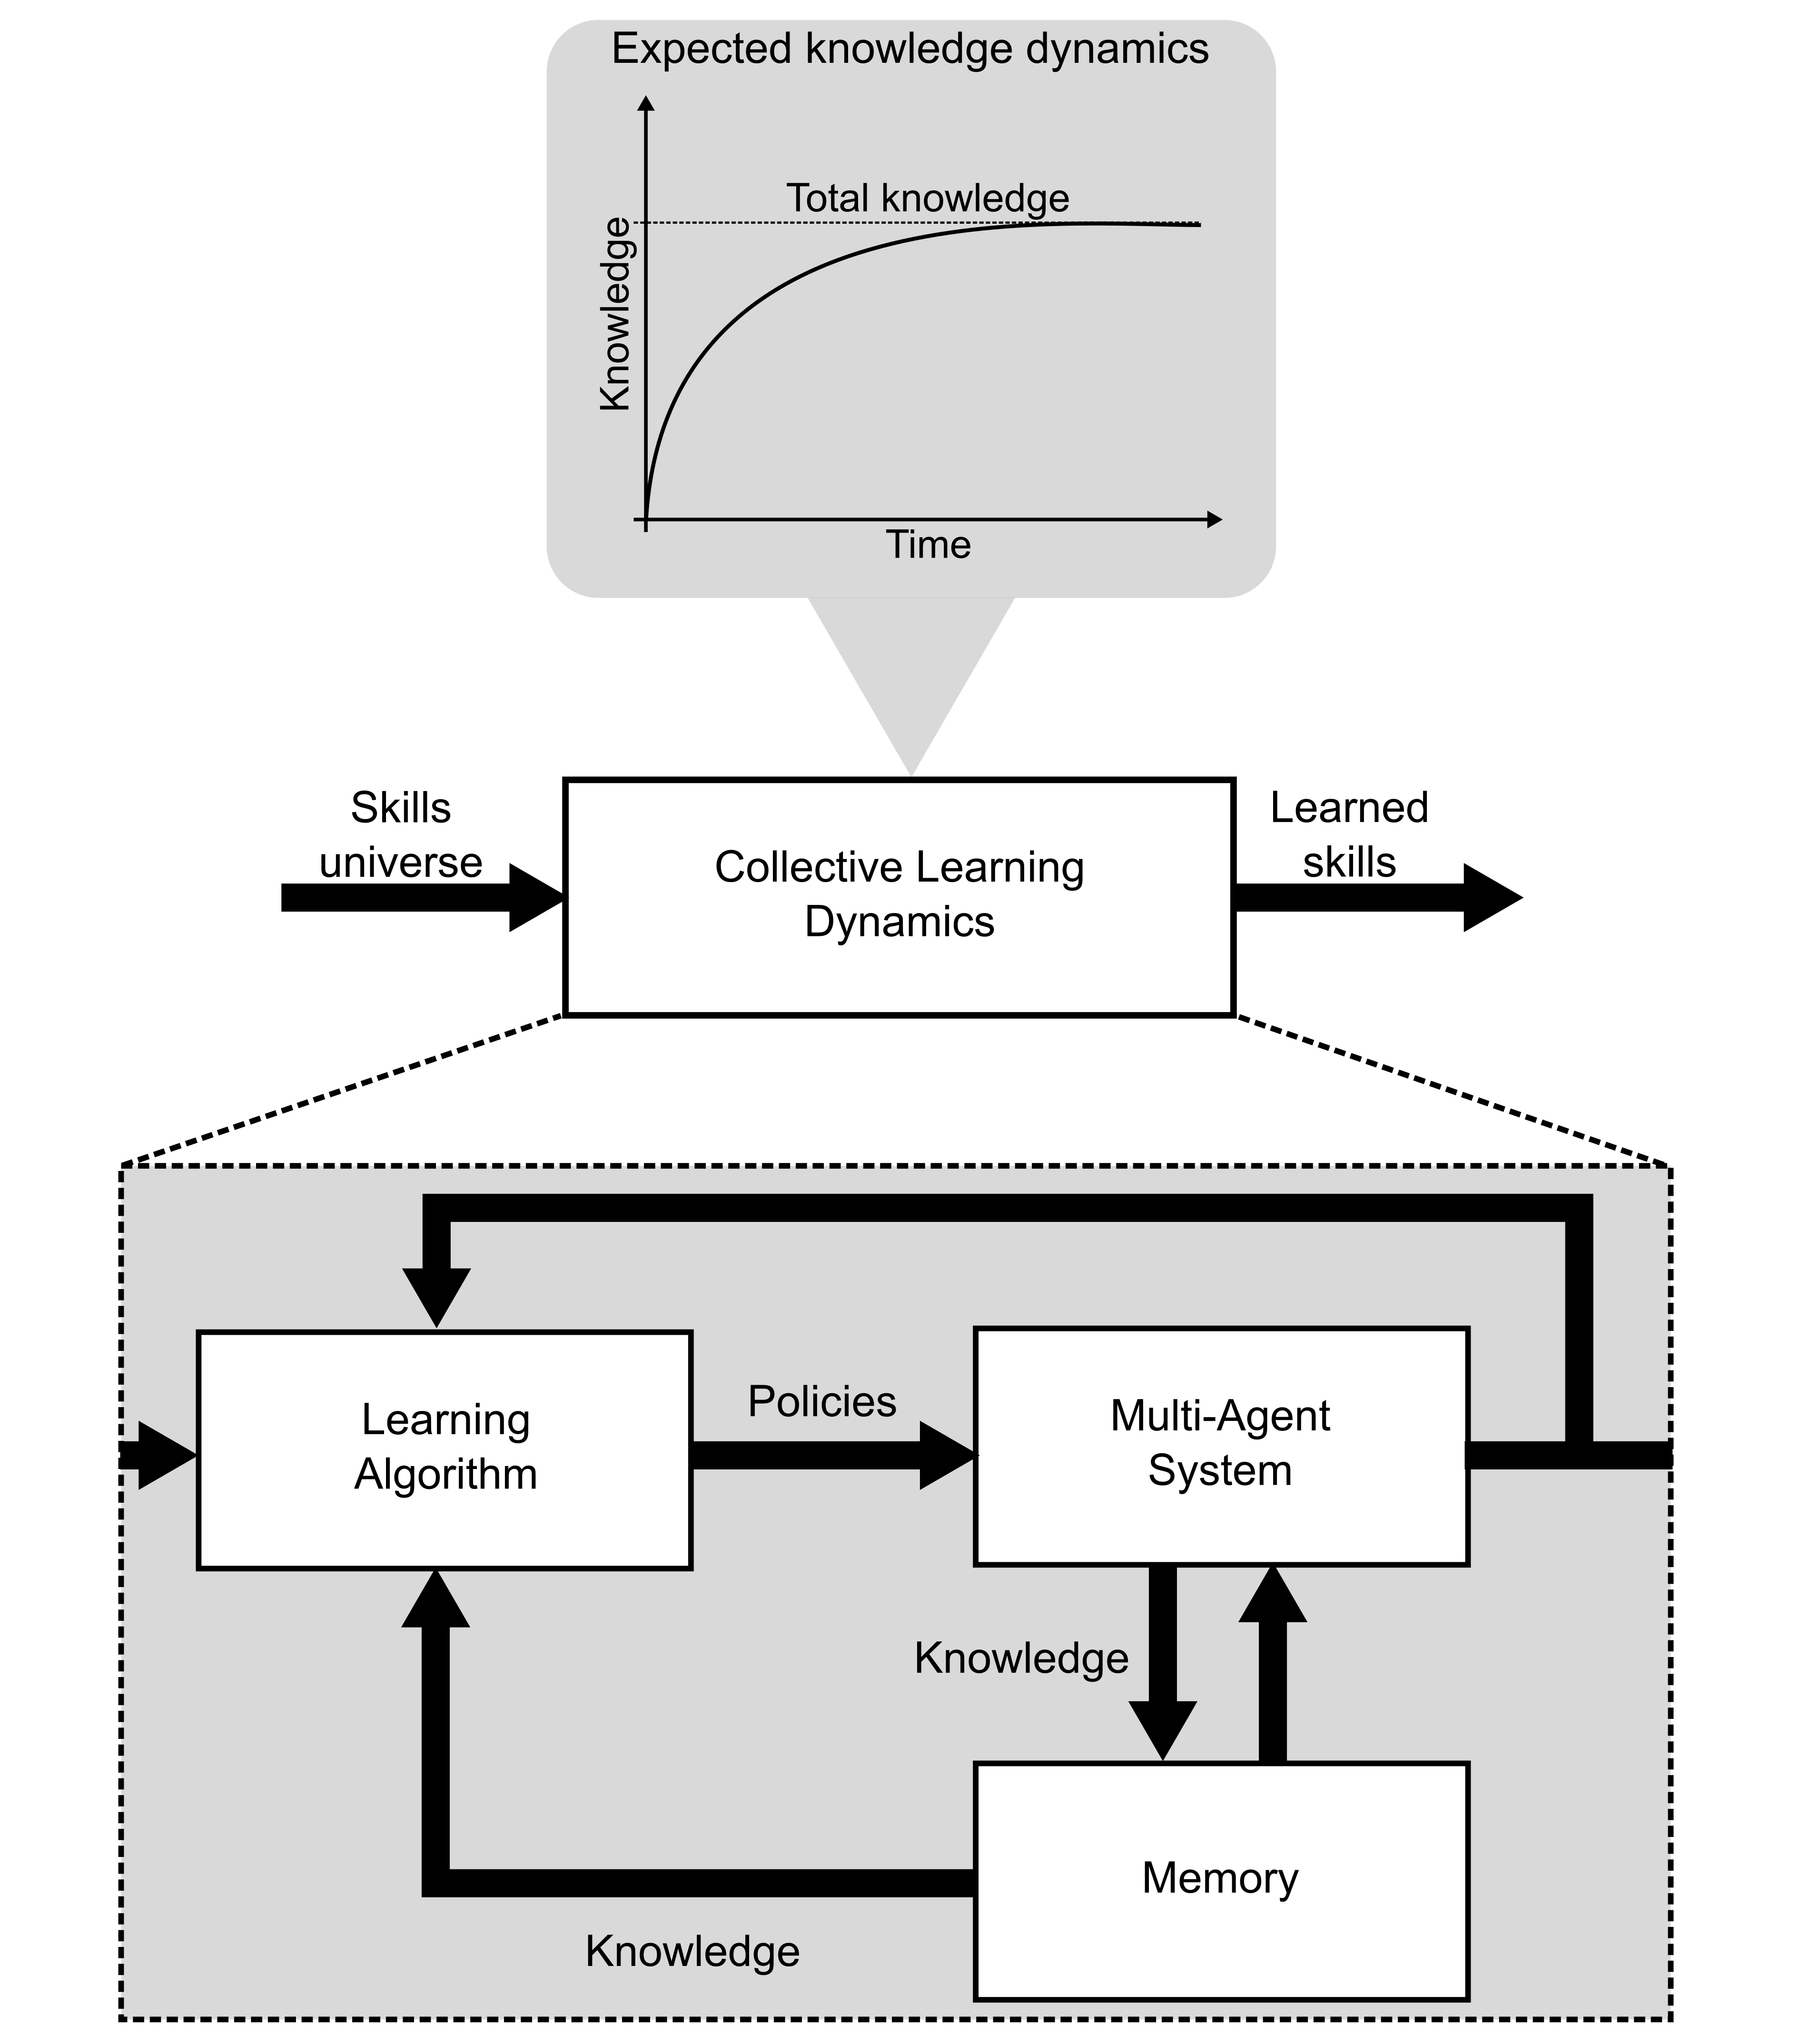
\includegraphics[width=14cm]{closed_loop_collective_dynamics.png}
	\hspace*{\fill}
	\caption[] {\label{fig:collective_learning_system} \textbf{A \acl{cl} system.} {A multi-agent system with appropriate learning algorithm(s) and inter-agent knowledge sharing can learn a universe of skills exponentially fast, as reflected by the exponential collection of the knowledge required to learn the skills.}\pending{Consider sending this figure to the supplementary materials.}}
\end{figure*}
% ---

The \ac{cl} concept encapsulates the dynamic, progressive creation and augmentation of knowledge through interactive processes. In this framework, knowledge from individuals is actively exchanged, spread, and enhanced, fostering a deeper, more comprehensive understanding that evolves over time \cite{Garavan2012CollectiveLearning}. Fundamental aspects of \ac{cl} that are particularly relevant to \ac{eai} agents include the aggregation of skills, knowledge, and behaviors. This concept is loosely related to collective intelligence and swarm intelligence \cite{Beni2004SwarmIntelligenceSwarm,Blum2015SwarmIntelligenceOptimization,Dorigo2021SwarmRoboticsPast} (which mostly focus on the emergence of coordinated behavior through a set of basic interaction rules), collaborative, federated, and distributed learning \cite{Technologie2023FLAIROPFederatedLearning,Anjos2023SurveyCollaborativeLearning,Xianjia2021Federatedlearningrobotic,Sartoretti2019DistributedLearningDecentralized,Sartoretti2018DistributedLearningDecentralized,Wang2022DistributedReinforcementLearning} (concepts dealing mainly with decentralizing computation and access to data), networked robotics \cite{Kumar2008NetworkedRobots} (whose scope is centered on the coordination and collaboration of multiple robotic agents), and fleet learning \cite{Wang2023RobotFleetLearning} (an approach more akin to parallel learning). Arguably, the many contributions in these areas have addressed various underlying principles of collective systems \cite{Kernbach2013HandbookCollectiveRobotics}.
Nevertheless, these approaches do not target the hypothesized exponential learning resulting from \ac{cl} \cite{Haddadin2019Breakingwallcollective}. Furthermore, the specific algorithms required to effectively realize \ac{cl}---in particular, for knowledge acquisition, transfer,  distribution, and integration---are still nonexistent or currently under development \cite{Haddadin2022collectivelearningtheory}. Despite this, the expectation is that an appropriate learning algorithm that can leverage the body of knowledge accumulated by a multi-agent system (a collective) can shape the knowledge acquisition dynamics of the whole system, positively impacting the learning time and energy efficiency of new skills, see Fig.~\ref{fig:collective_learning_system}.
¸
% ===================================================================================================
%                                                 |                                                 |
%                                                 |                                                 |
% -------------------------------------------- SECTION ---------------------------------------------|
%                                                 |                                                 |
%                                                 |                                                 |
% ===================================================================================================
\section*{Modeling the dynamics of skill knowledge}\label{sec:knowledge_dynamics_model}
Understanding the energy and time demands represented by a team of $m$ robots learning a universe $\mathcal{S}=\left\lbrace s_1,s_2,\ldots s_j,\ldots, s_{N_\mathcal{S}}\right\rbrace$ of skills, with $|\mathcal{S}| = N_\mathcal{S}$, requires looking at how knowledge about a skill is gained and what effect it can have on the acquisition of any new skill knowledge. 

To start, we consider that the \emph{complexity} $c_j$ of a skill $ s_j $ is the number of trial episodes $n$ needed to successfully learn the skill, i.e., all actions and states visited by an \ac{eai} agent until a stopping criterion is reached. Additionally,
% ---
\begin{tcolorbox}
	\begin{assumption}\label{assumption:power_and_episode_time}
		the average behavior of a system where both $m$ and $N_\mathcal{S}$ are large can be described by the power $P_0$ required by any agent during learning and the mean execution time $\Delta t$ of every trial episode $n$, with both approximately constant; see Fig.~\ref{fig:power_per_episode}.
	\end{assumption}
\end{tcolorbox}
% ---
\noindent As a consequence of Asm.~\ref{assumption:power_and_episode_time}, and according to Eqs.~\eqref{eq:energy_per_episode},\eqref{eq:energy_per_skill}, and \eqref{eq:total_energy} in Sec.~\ref{sec:power_per_episode}, the energy demand of an \ac{eai} agent learning a skill (or set of skills) is proportional to the skill(s) complexity.

% ===================================================================================================
\paragraph*{Similarity and knowledge}
Let $\mathcal{Z}_k \subset \mathcal{S}$ be a subset of $N_{\mathcal{Z}_k}$ highly similar skills; that is, a \emph{cluster} of similar skills, see Fig.~\ref{fig:skill_similarity}. Furthermore, consider a second set $\mathcal{\zeta}_k \subset \mathcal{Z}_k$ that denotes the skills from $\mathcal{Z}_k$ that a given agent has already learned. Furthermore, we make the assumption that  
%---
\begin{tcolorbox}
	\begin{assumption}\label{assumption:skill_clustering} if the similarity among a set of skills is significant, exchanging acquired knowledge from these skills expedites the overall learning process.
	\end{assumption}
\end{tcolorbox}
% ---
\noindent This implies that the $j$-th skill in the $k$-th cluster $s_{j,k} \in \mathcal{Z}_k$ can always benefit from the knowledge contained in $\mathcal{\zeta}_k$. Consequently, the more skills in $\mathcal{\zeta}_k$, the less knowledge about $ s_{j,k} $ remains to be learned. To model this effect, we introduce a function $\bar{\sigma}_{j,k}\left(n\right)\in [0,1]$ that expresses the knowledge about a skill $s_{j,k} \in \mathcal{Z}_k \setminus \mathcal{\zeta}_k$ that \emph{is not} contained in the knowledge base of $\mathcal{\zeta}_k$. The function $\bar{\sigma}_{j,k}(\cdot)$ satisfies
% ---
\begin{equation}\label{eq:sigma_bar_conditions}
	\bar{\sigma}_{j,k}\left(n\right) = 
	\begin{cases}
		1 & \text{$\mathcal{\zeta}_k=\emptyset$},\\
		0 &\text{$\mathcal{\zeta}_k$ has \emph{all} knowledge of $s_{j,k}$}.
	\end{cases}
\end{equation}
% ---
Conceptually, $\bar{\sigma}_ {j,k}\left(\cdot\right)$ is the fraction of knowledge from ${\mathcal{Z}_k}$ that remains to be learned.
% ---
\begin{figure*}[!t]
	\centering
	\hspace*{\fill}
	\begin{subfigure}[t]{0.45\textwidth}
		\subcaption{}
		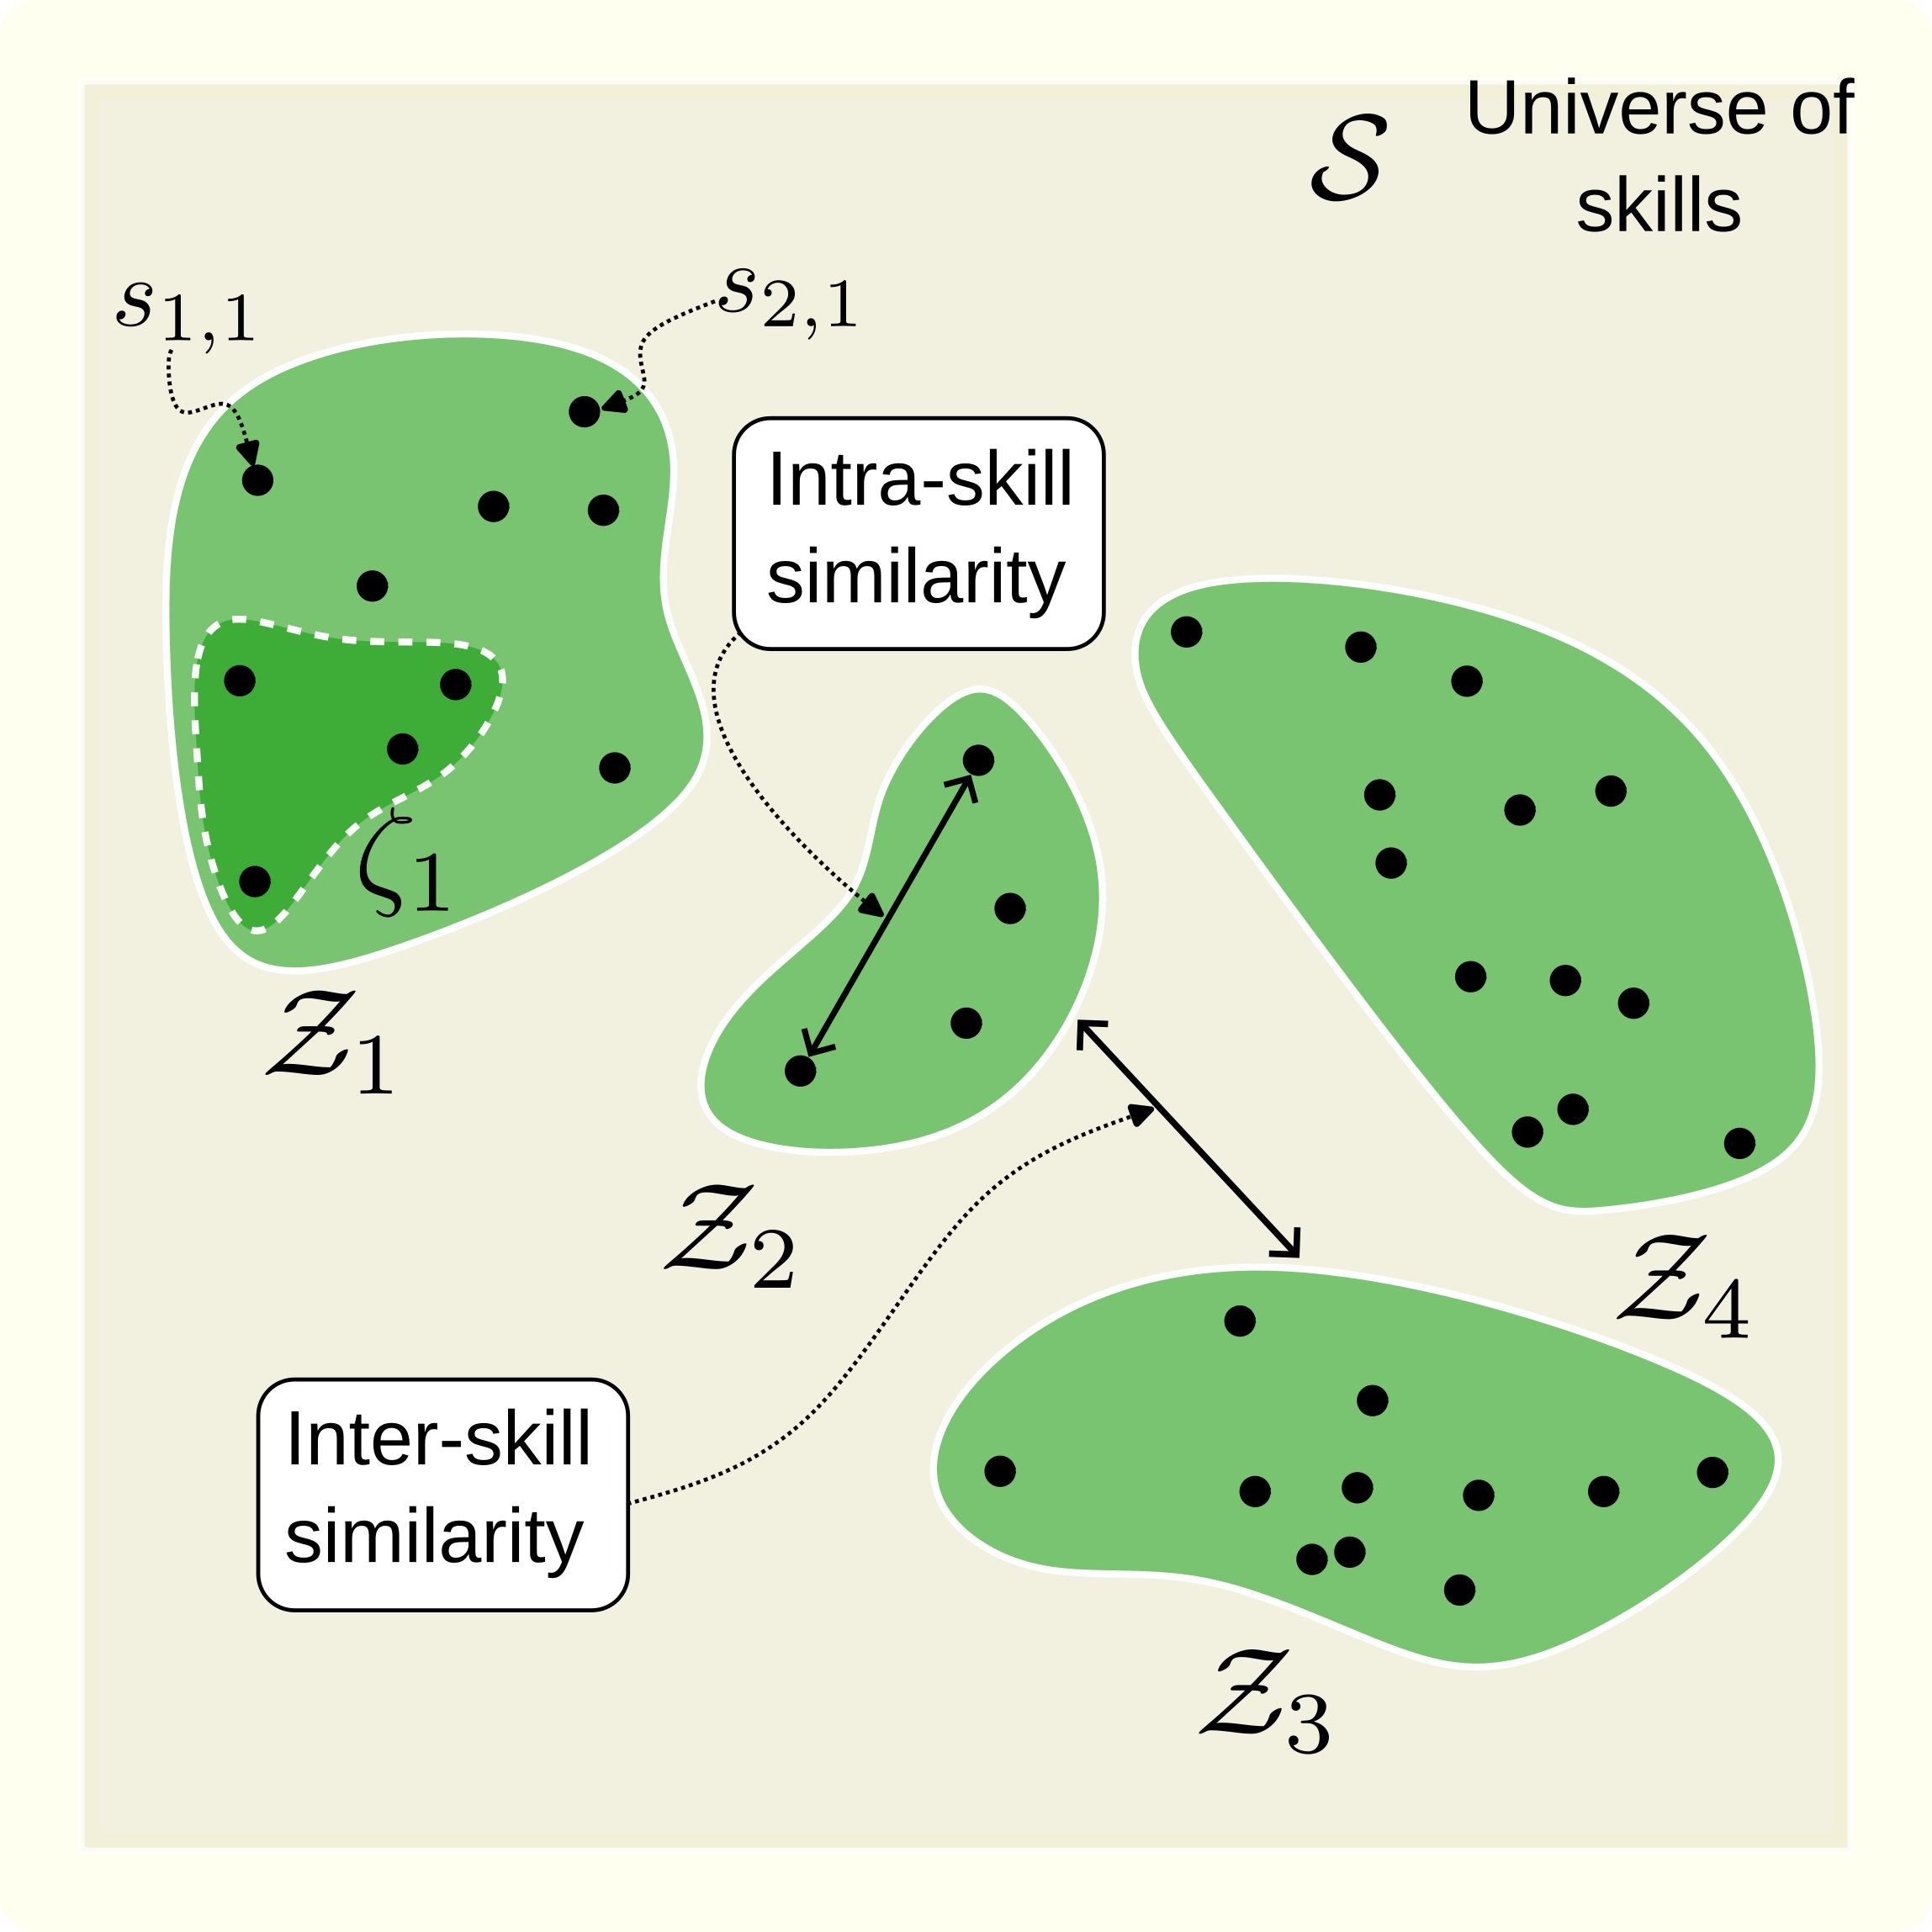
\includegraphics[width= \textwidth]{skill_similarity.png} \label{fig:skill_similarity}
	\end{subfigure}
	\hfill
	%\begin{subfigure}[t]{wid0.48\textwidth}
	\begin{subfigure}[t]{8.35cm}	
		\subcaption{}
		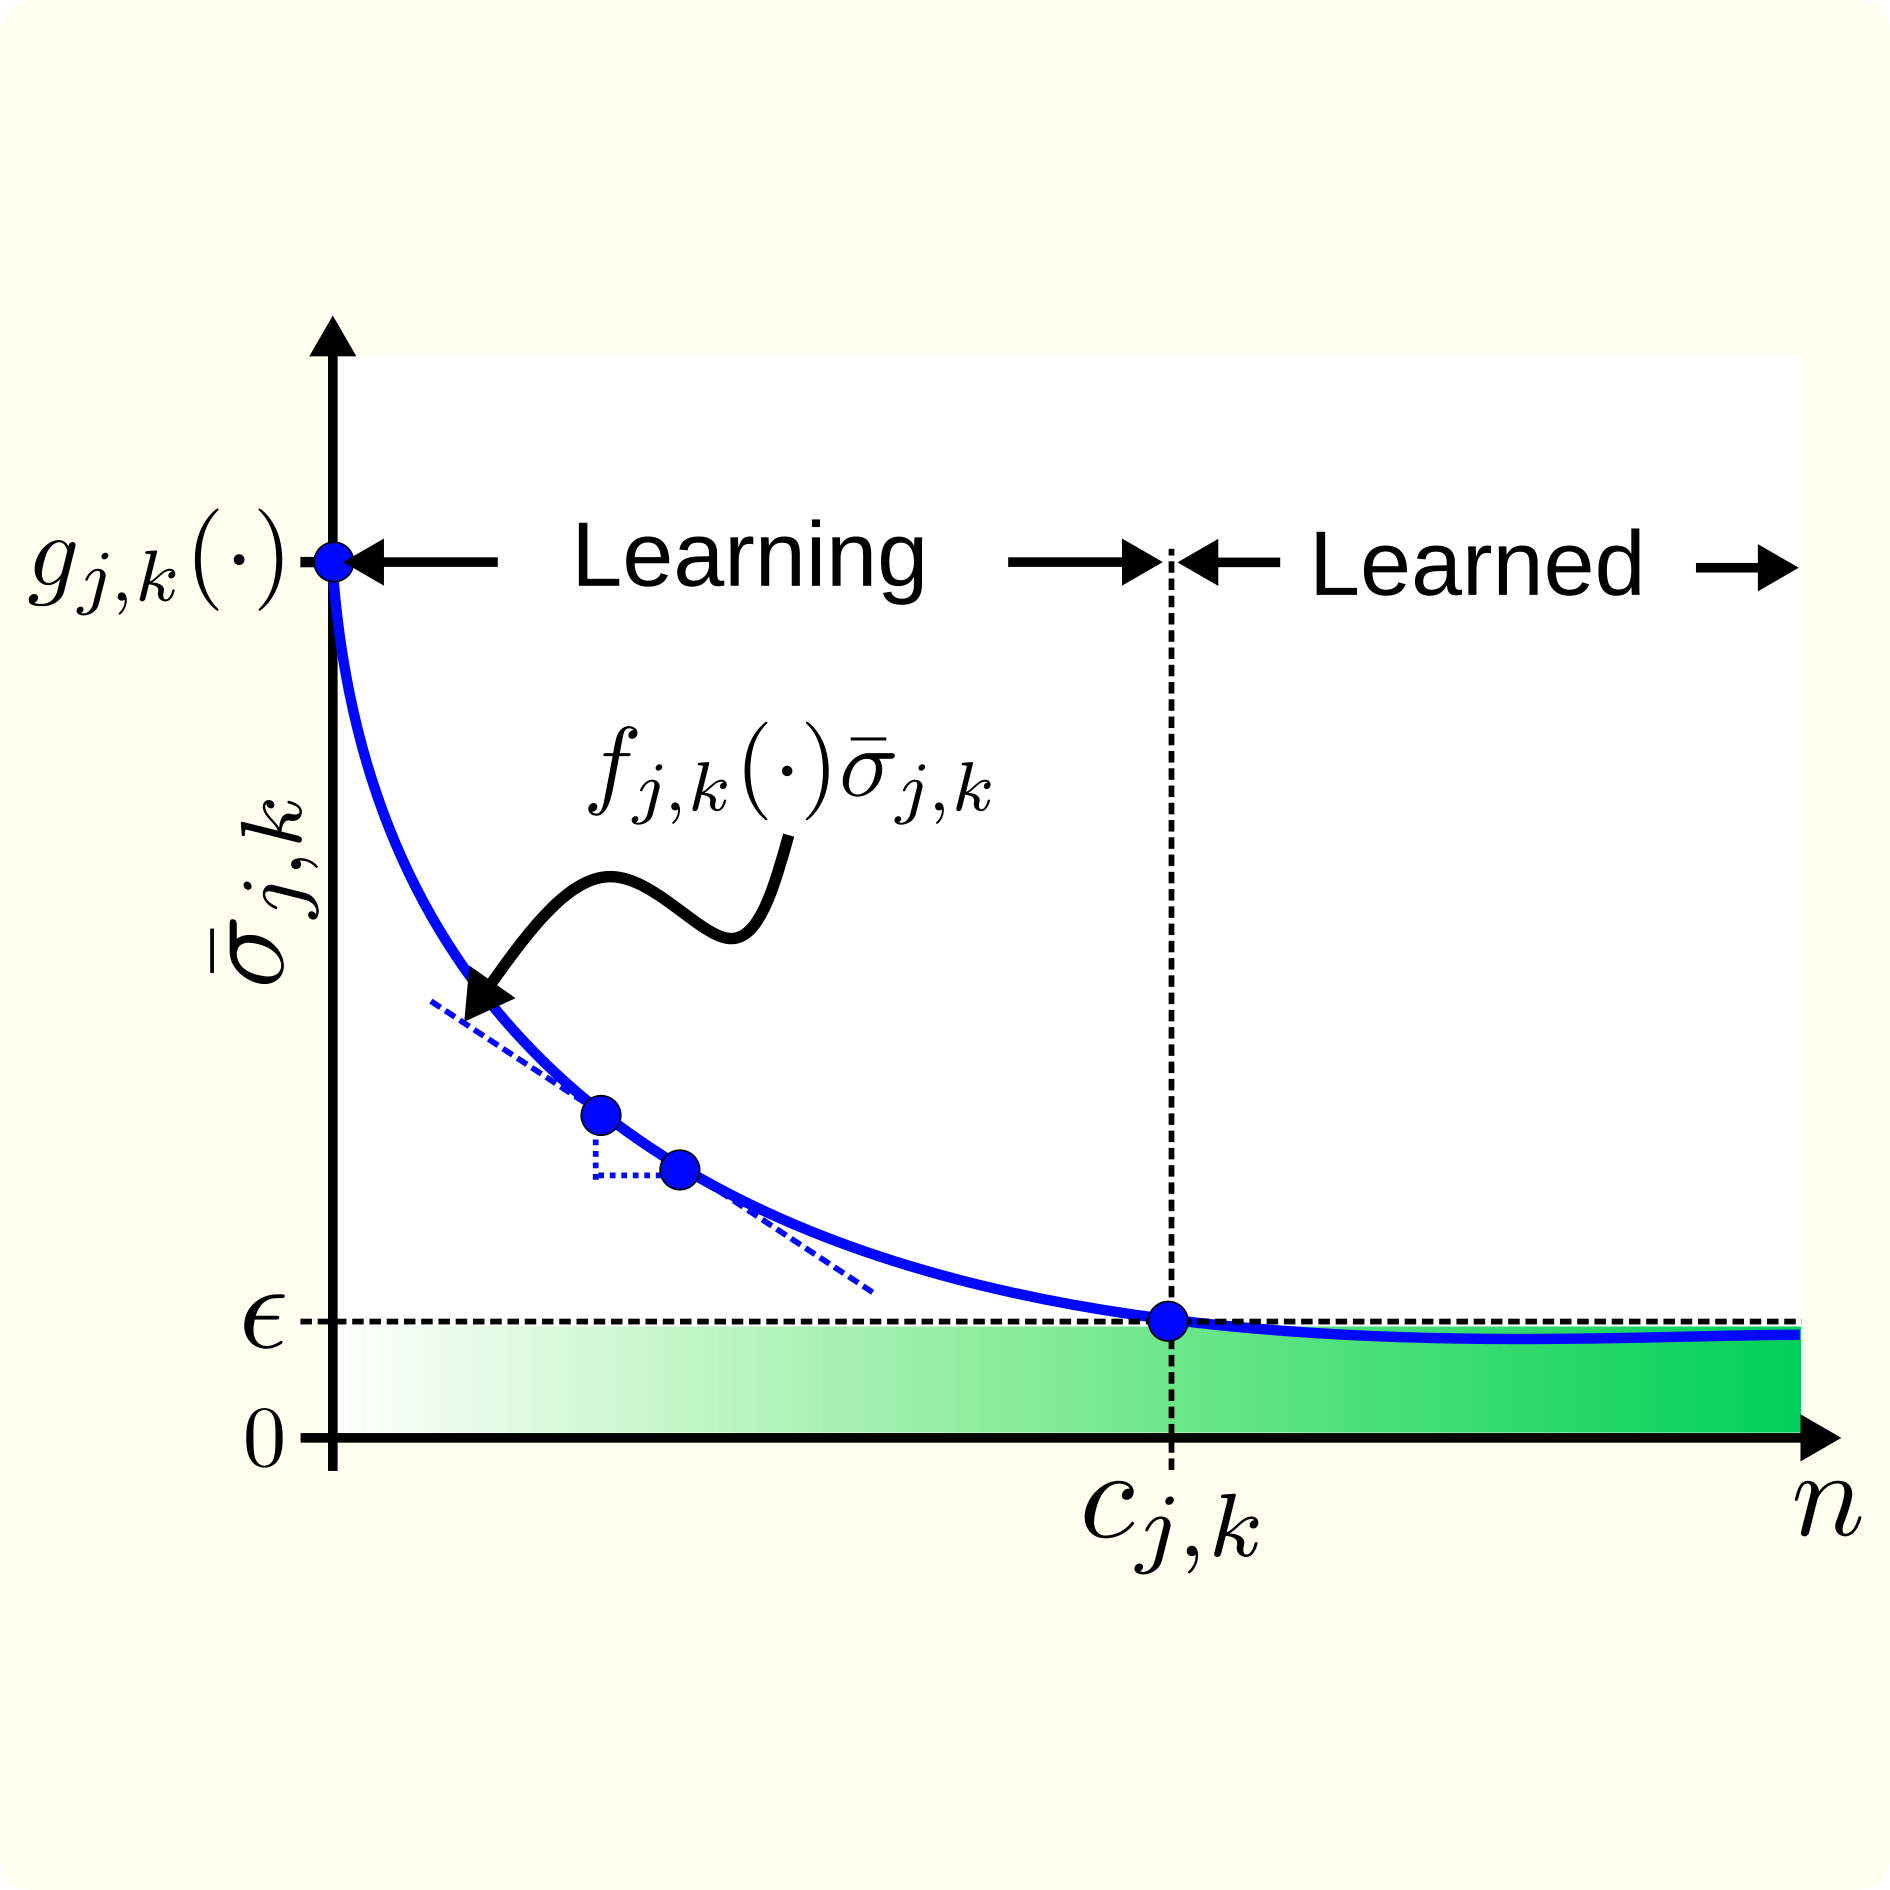
\includegraphics[width=8.35cm]{remaining_knowledge_dynamics_idealization.png} \label{fig:knowledge_idealization}
	\end{subfigure}
	\hspace*{\fill}
	\caption[] {\label{fig:experimental_results} \textbf{Skill similarity and knowledge.} (\subref{fig:skill_similarity}) Similar skills in $\mathcal{S}$ can be grouped into clusters $\mathcal{Z}_k$, (\subref{fig:knowledge_idealization}) the remaining knowledge $\bar{\sigma}_{j,k}$ to learn a new skill $s_{j,k}$ has a monotonically decreasing behavior.}	
\end{figure*}
% ---
% ===================================================================================================
\paragraph*{Leveraging the acquired knowledge}
To evaluate the effect of knowledge exchange during learning on the complexity of mastering a skill, we introduce a hypothetical upper bound called the skill \textit{fundamental complexity} $c_0$, which describes the maximum number of trial episodes required to learn \emph{any} skill. If, in learning a skill $ s_{j,k} $, an \ac{eai} agent can access and use the knowledge contained in $\mathcal{\zeta}_k$, then two effects take place:
% ---
\begin{enumerate}
	\item There is less remaining knowledge, reflected in the initial value; i.e., $\bar{\sigma}_{j,k}(0) < 1$
	\item The knowledge acquisition rate increases. This can also be interpreted as an increase in the depletion rate of the remaining knowledge.
\end{enumerate}
% ---
These effects signify that the remaining knowledge scales down as a function of the number of learned skills $N_{\zeta_k}=|\mathcal{\zeta}_k|$. Consequently, the complexity $c_{j,k}$ of said skill is smaller than the fundamental complexity $c_0$. Additionally, without loss of generality, under knowledge exchange, we can consider that
% ---
\begin{tcolorbox}
	\begin{assumption}\label{assumption:exponential_decrease} the remaining knowledge function $\bar{\sigma}_{j,k}(\cdot)$ has a monotonically decreasing behavior.
	\end{assumption}
\end{tcolorbox} 
% ---
\noindent An idealization of the behavior satisfying Asm.~\ref{assumption:exponential_decrease} and Eq.~\eqref{eq:sigma_bar_conditions} can be modeled via a differential equation depending on the trial episodes $n$ and parameterized by the number of already learned skills $N_{\zeta_k}$. As such,
% ---
\begin{definition}\label{assumption:ode_model} the remaining knowledge function $\bar{\sigma}_{j,k}$ is modeled as the first order dynamical system
%	\begin{subequations}\label{eq:simple_knowledge_dynamics}
%		\begin{empheq}[left=\empheqlbrace]{align}
%			\dot{\bar{\sigma}}_{j,k}\left(n\right) &  = -f_{j,k} \left(N_{\zeta_k} \right) \bar{\sigma}_{j,k}\left(n\right),\\
%			\bar{\sigma}_{j,k}(0) &  =  g_{j,k} \left(N_{\zeta_k}\right).
%		\end{empheq}
%	\end{subequations}
	\begin{equation}\label{eq:simple_knowledge_dynamics}
		\dot{\bar{\sigma}}_{j,k}\left(n\right)=\begin{cases}
			-f_{j,k} \left(N_{\zeta_k} \right) \bar{\sigma}_{j,k}\left(n\right), & \epsilon < \bar{\sigma}_{j,k}\left(n\right) < 1, \\
			0, & \text{otherwise}.
		\end{cases}
	\end{equation}	
\end{definition}
% ---
\noindent Considering its initial condition as $\bar{\sigma}_{j,k}(0) =  g_{j,k} \left(N_{\zeta_k}\right)$, the corresponding solution
% ---
\begin{equation}\label{eq:knowledge_exponential_form}
	\bar{\sigma}_{j,k}(n) = g_{j,k}(N_{\zeta_k}) e ^{-f_{j,k}\left(N_{\zeta_k}\right) n} \in (0,1],
\end{equation}
% ---
exhibits the desired behavior, shown in Fig.~\ref{fig:knowledge_idealization}. The function $f_{j,k}\left(N_{\zeta_k}\right)$ models one of the effects resulting from the exploitation of the knowledge available in $\zeta_k$, namely, the increase of the learning rate. The second effect, namely, the reduction in the initial remaining knowledge $\bar{\sigma}_{j,k}(0)$ is controlled by the term $g_{j,k}\left(N_{\zeta_k}\right)$, which is also dependent on the number of learned skills. The learning threshold $\epsilon$---depicted as the green-shaded area in Fig.~\ref{fig:knowledge_idealization}---indicates when the remaining knowledge is negligible and $s_{j,k}$ is considered as learned.

% ===================================================================================================
%                                                 |                                                 |
%                                                 |                                                 |
% -------------------------------------------- SECTION ---------------------------------------------|
%                                                 |                                                 |
%                                                 |                                                 |
% ===================================================================================================
\section*{Knowledge sharing under different learning paradigms}
For the upcoming analysis, we consider an idealized reference system in which many robots coexist, learning numerous skills. Such system exhibits
% ---
\begin{tcolorbox}
	\begin{assumption}\label{assumption:average_behavior}
		an average behavior that results from comparable \ac{eai} agents learning and executing the skills in $\mathcal{S}$ ordered and segregated according to their similarity.
	\end{assumption}
\end{tcolorbox}
%---
\noindent Each of the \ac{eai} agents in the system
\begin{tcolorbox}
	\begin{assumption}\label{assumption:agent_similarity}
		has the same capabilities, with highly similar \ac{bee} and \ac{mie} expenditures.
	\end{assumption}
\end{tcolorbox}
%---
\noindent The large number of skills in $\mathcal{S}$ implies that
% ---
\begin{tcolorbox}
	\begin{assumption}\label{assumption:cluster_size}
		every cluster $\mathcal{Z}_{k}$ contains the same number $N_{\mathcal{Z}} $ of skills.
	\end{assumption}
\end{tcolorbox}
% ---
\noindent By virtue of the optimal ordering of the skills and the balanced size of the clusters,
% ---
\begin{tcolorbox}
	\begin{assumption}\label{assumption:cluster_transferability}
		the knowledge transferability between in-cluster skills---modeled by Eq.~\eqref{eq:f_function_incremental} and Eq.~\eqref{eq:g_function_incremental}---is assumed to be equal; as is transferability between clusters, see Eq.~\eqref{eq:f_function_transfer} and Eq.~\eqref{eq:g_function_transfer}.
	\end{assumption}
\end{tcolorbox}
% ---
\noindent Finally, the different learning paradigms that exploit the collected knowledge by the \ac{eai} agents rely on the assumption that
% ---
\begin{tcolorbox}
	\begin{assumption}\label{assumption:enabling_agorithms}
		there are advanced control and machine learning algorithms designed to inherently use this knowledge.
	\end{assumption}
\end{tcolorbox}
% ---

% ---
\begin{figure*}[!t]
	\centering
	\hspace*{\fill}
	\begin{subfigure}[t]{0.32\textwidth}
		\subcaption{}
		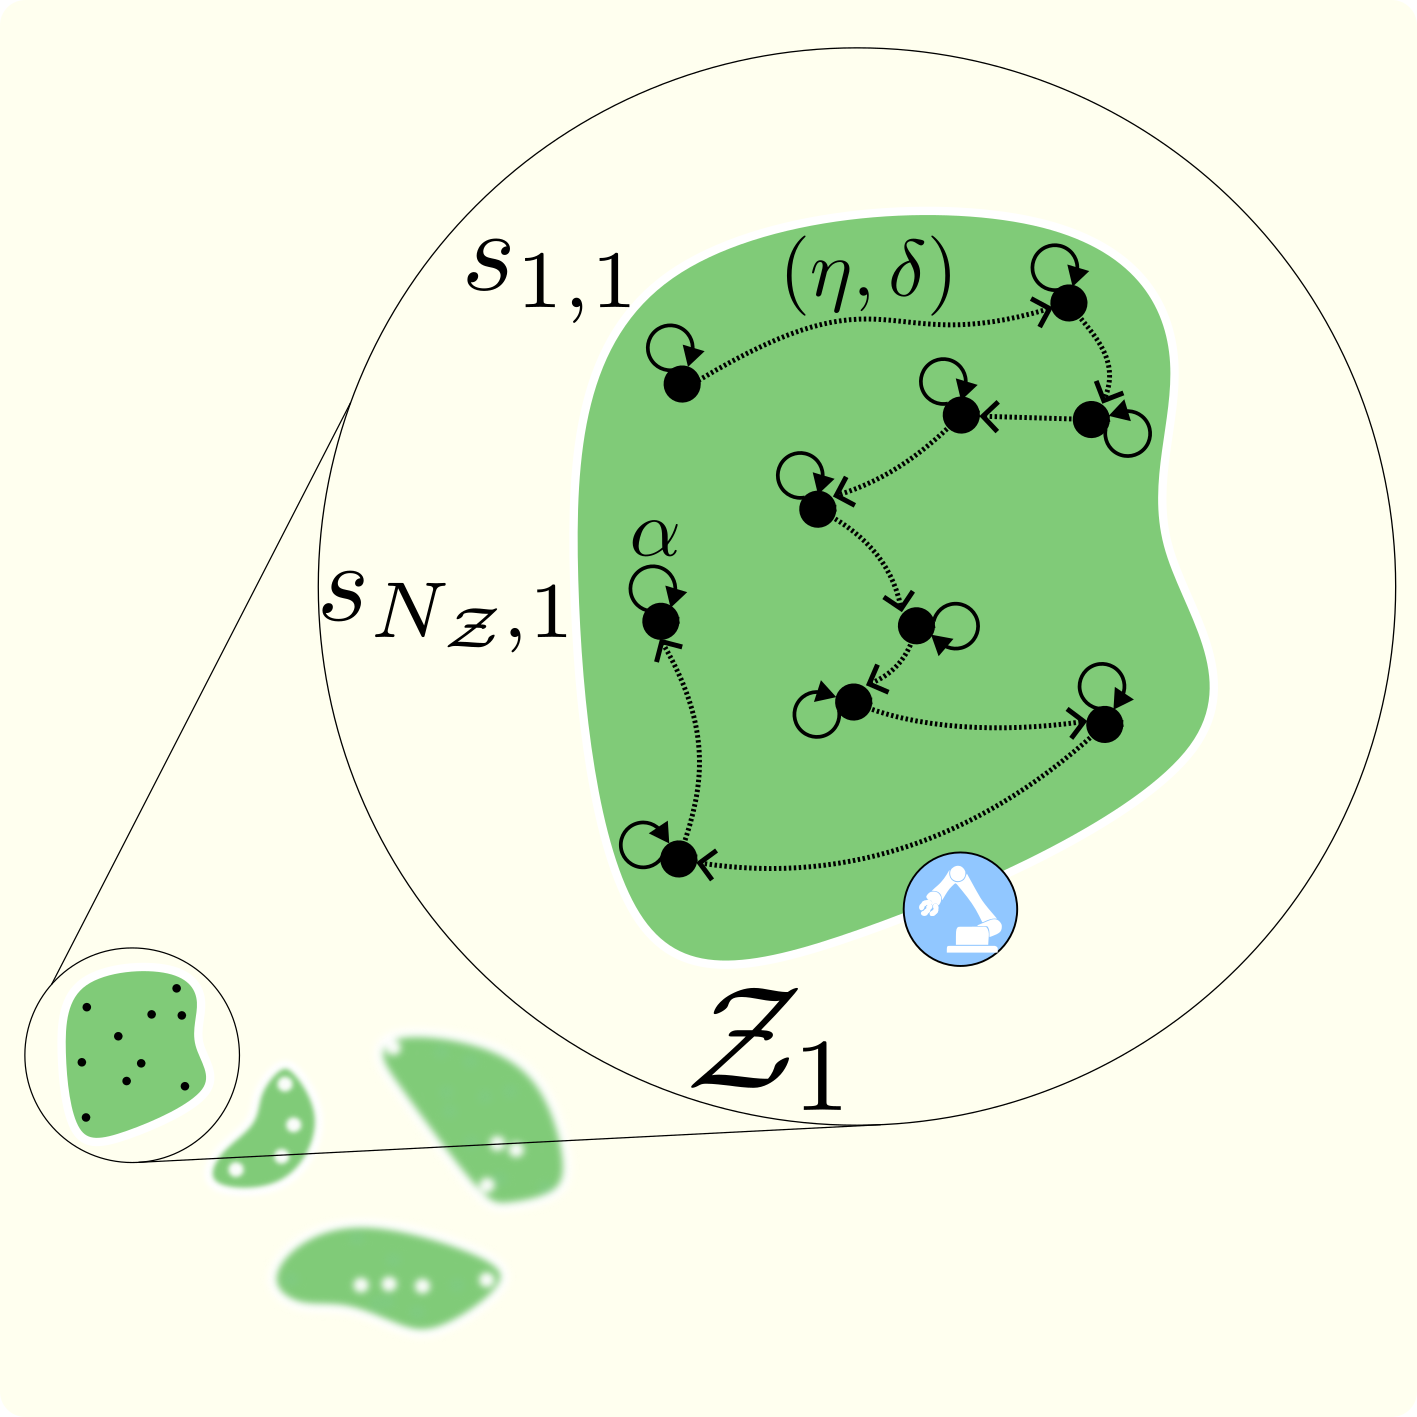
\includegraphics[width= \textwidth]{intra_skill_learning.png} \label{fig:intra_skill_learning}
	\end{subfigure}
	\hfill
	\begin{subfigure}[t]{0.32\textwidth}
		\subcaption{}
		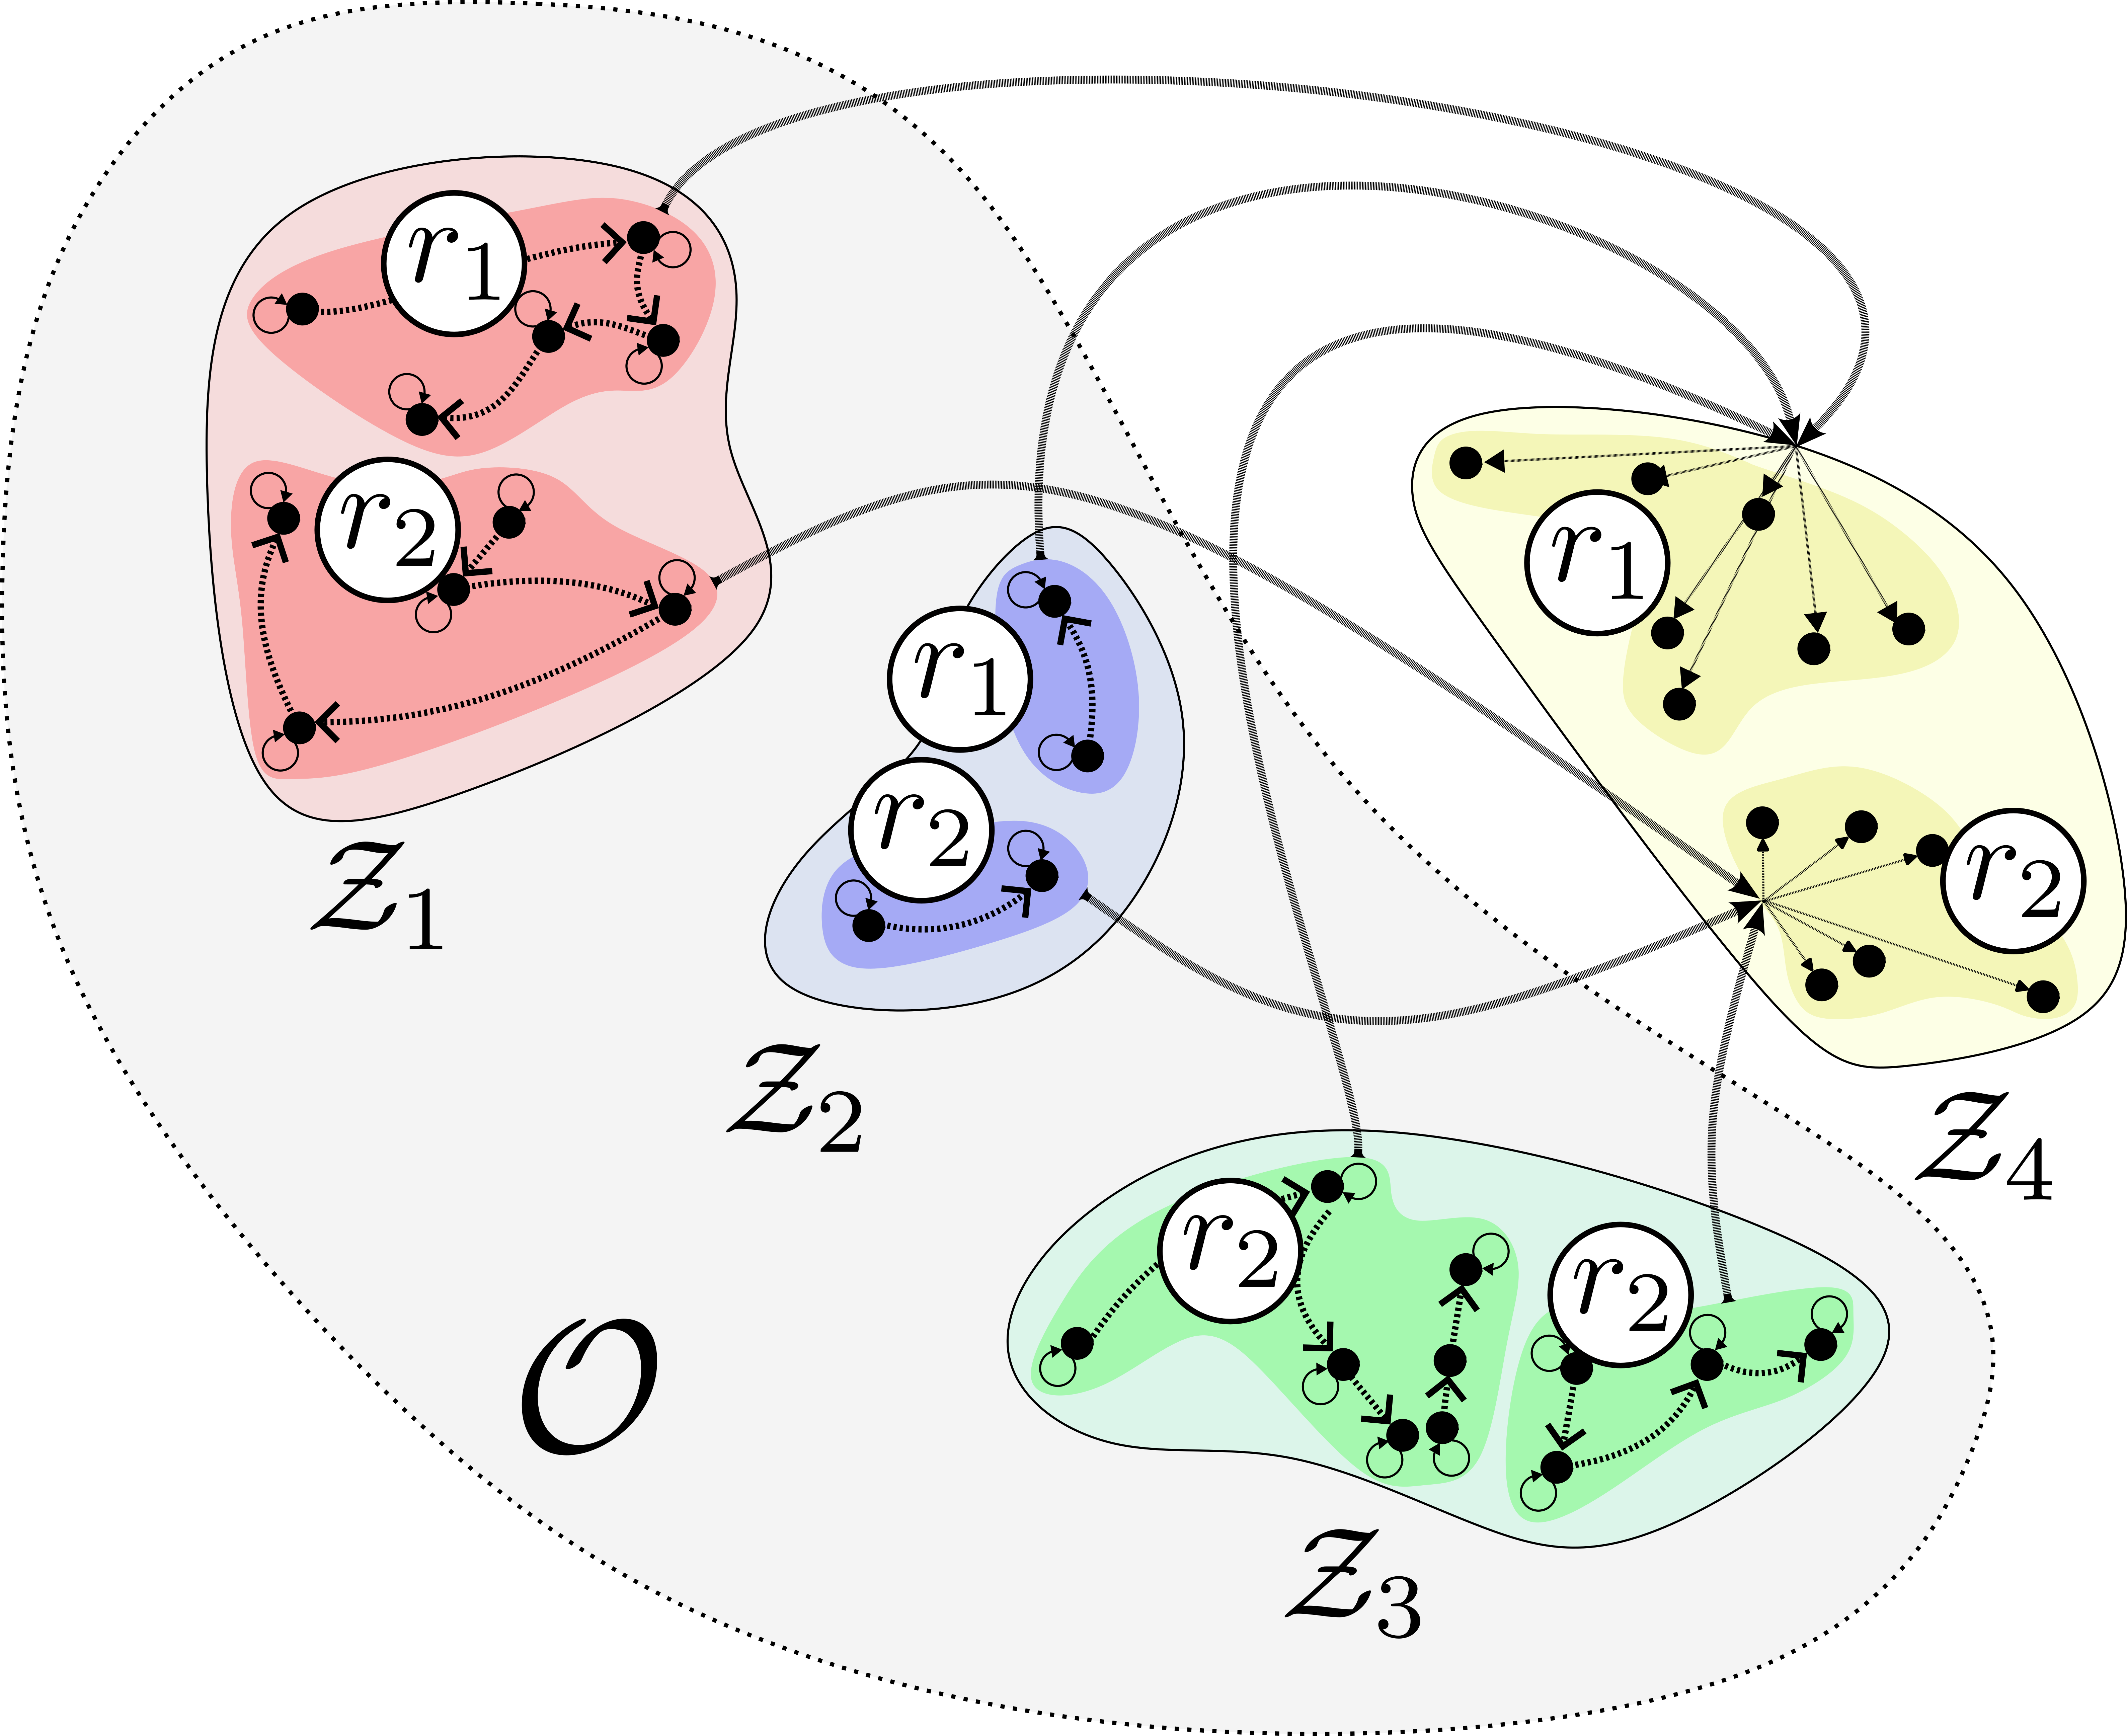
\includegraphics[width=\textwidth]{cluster_to_cluster_knowledge_transfer_parallel.png} \label{fig:cluster_to_cluster_knowledge_transfer_parallel}
	\end{subfigure}
	\hfill
	\begin{subfigure}[t]{0.32\textwidth}
		\subcaption{}
		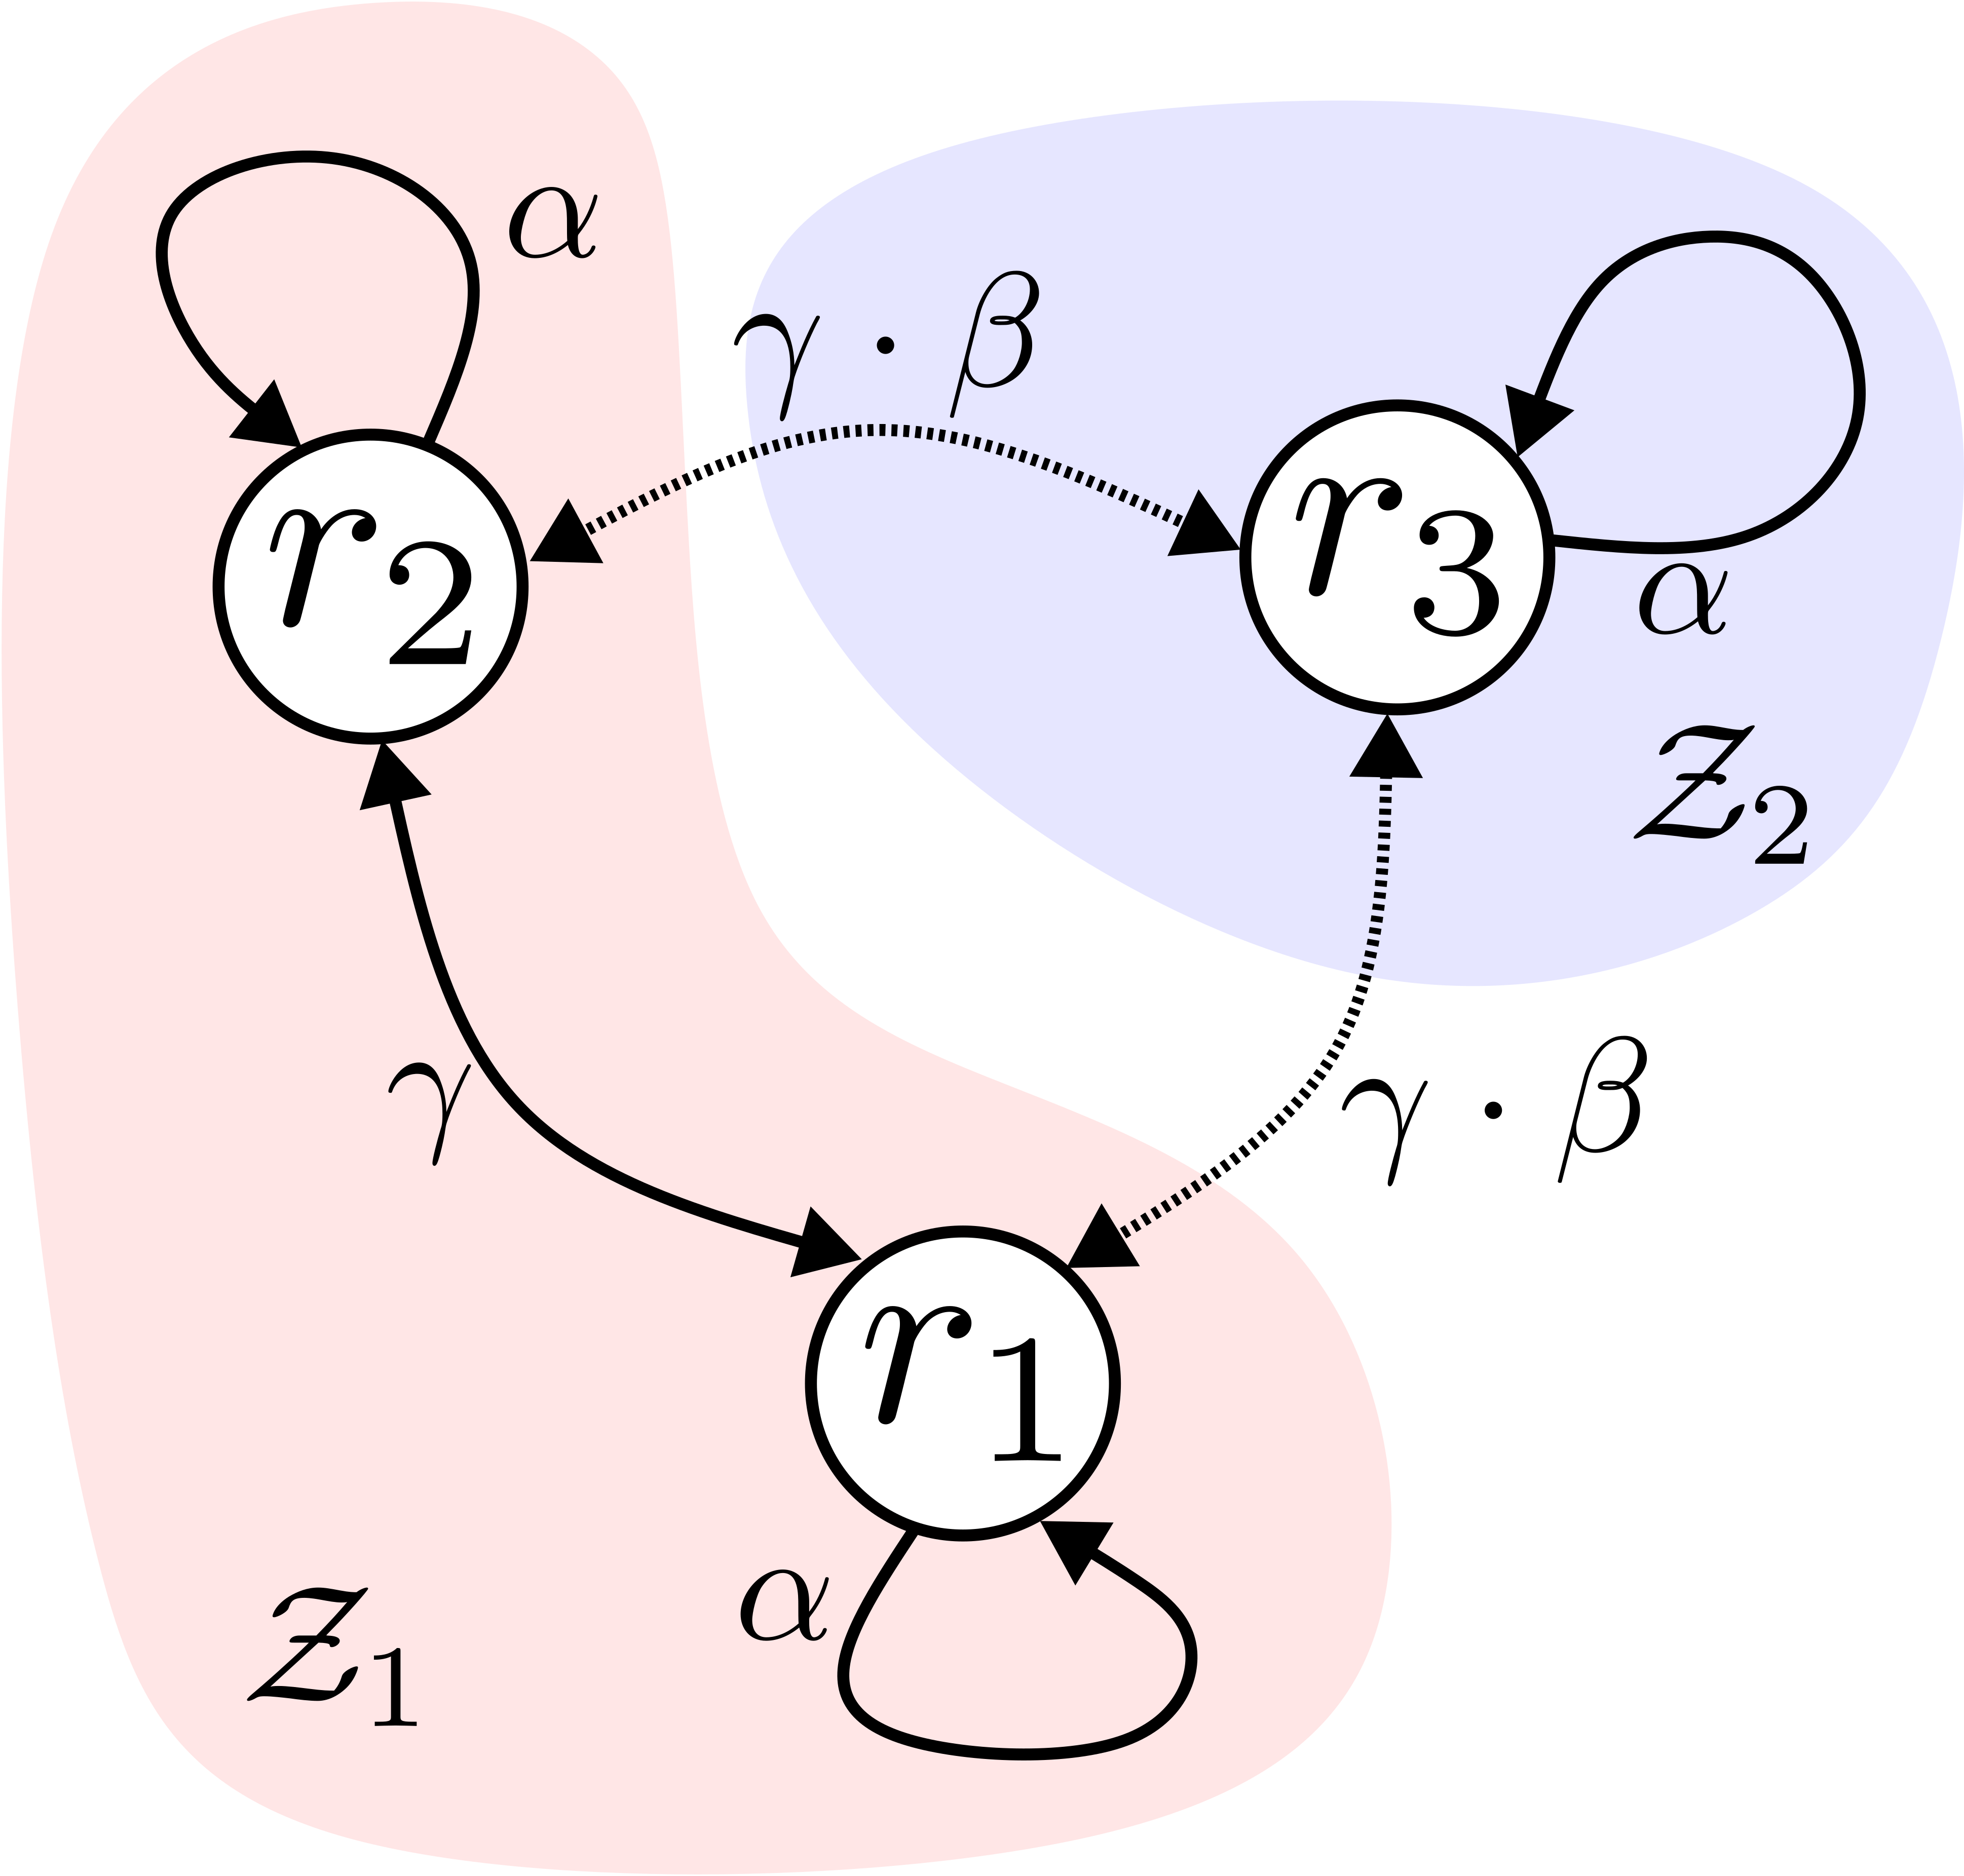
\includegraphics[width=\textwidth]{cl_example_figure.png} \label{fig:cl_example_figure}
	\end{subfigure}	
	\hspace*{\fill}
	\caption[] {\label{fig:learning_paradigms_conceptual_figure} \textbf{The different learning paradigms.} (\subref{fig:intra_skill_learning}) Incremental learning benefits from the significant similarity of skills belonging to the same cluster. (\subref{fig:cluster_to_cluster_knowledge_transfer_parallel}) In transfer learning, knowledge is shared from different origin clusters to the target cluster. Notice that using many robots (e.g., two robots $r_1$ and $r_2$) without inter-agent knowledge exchange among them only subdivides the problem. (\subref{fig:cl_example_figure}) Exchange of knowledge between \ac{eai} agents enables collective learning.}
\end{figure*}
% ---

% ===================================================================================================
\paragraph*{Conventional learning paradigms} 
When an \ac{eai} agent performs \ac{isl}, it learns each new skill from the ground up, disregarding the accumulating knowledge from already learned skills. In contrast, \ac{il}---also known as continual learning \cite{Lesort2020Continuallearningrobotics}---corresponds to the case where an agent benefits from the continuous aggregation and exchange of knowledge from \emph{intra-cluster} skills in virtue of their significant similarity. As depicted in Fig.~\ref{fig:intra_skill_learning}, a robot ($r_1$ in this case) learns every skill in $\mathcal{Z}_1$ with a rate $\alpha$---the self-loops---but also retains and uses the acquired knowledge to learn subsequent skills. \Ac{tl} alone refers to the use of acquired knowledge about a set of skills on a new skill \cite{Hosna2022Transferlearningfriendly,Jaquier2023TransferLearningRobotics}. In particular, it implies the one-time \emph{inter-cluster} exchange of knowledge. \Ac{tl} represents the exchange of knowledge from the skills learned in different \emph{origin} clusters $\mathcal{O} = \{ \mathcal{Z}_1,\mathcal{Z}_2,\ldots,\mathcal{Z}_{k-1} \}$ to the skills that will be learned in a \emph{destination} cluster $\mathcal{Z}_k$ (see Fig.~\ref{fig:cluster_to_cluster_knowledge_transfer_parallel}). Concretely, the effect that \ac{tl} has on the skills of the destination cluster is the reduction of the initial remaining knowledge and the increase of the initial learning rate for all the skills in the $k$-th cluster via the \emph{aggregated and scaled cluster transferable knowledge fraction}~%\emph{transferable knowledge fraction factor}
$\xi_k \in [0,1)$. Which results from adding the transferable knowledge fraction $\varsigma_{k}$ from the $N_\mathcal{K}$ clusters scaled by the the \emph{cluster similarity matrix}
% ---
\begin{equation}\label{eq:cluster_similarity_matrix}
	\bm{B}=\begin{cases}
		1, & i=j, \\
		\beta_{ij} = \beta_{ji}, & i \neq j,
	\end{cases}
\end{equation}
% ---
with $\beta_{ij} \in [0,1)$ defines the closeness between the skills in the different clusters. In general, \ac{il} and \ac{tl} can always be combined; as such, we consider \ac{til} as the third learning paradigm. A complementary discussion on the effects that these paradigms have on the skill complexity is provided in Sec.~\ref{sec:materials_and_methods}.





% ===================================================================================================
\paragraph*{\textbf{\Acl{cl}}}
This paradigm goes beyond simple parallelization---learning different skills with different robots at the same time. In \ac{cl} $m$ robotic agents $ \left\lbrace r_i \right\rbrace_{i=1}^{m} $ develop and accumulate a common mind (body of knowledge) dynamically via networked interactions where individual experience, knowledge, and skills are disseminated to all the other elements in the collective \cite{Garavan2012CollectiveLearning}. Information flows vertically as previous knowledge is passed on and horizontally by sharing concurrent experience between agents. Knowledge can be replicated, complemented, and further developed via these mechanisms. Moreover, to enable \ac{cl}, it is assumed that an inter-agent communication protocol and the appropriate infrastructure are in place that allow agents to concurrently exchange and integrate the self-acquired and incoming knowledge to incrementally speed up the learning of all the agents as a whole. As a result, concurrent intra- and inter-cluster knowledge sharing is possible. Naturally, a complex scheduling problem to determine the optimal skill distribution and inter-agent knowledge-sharing strategy is part of the \ac{cl} paradigm. 

Rather than focusing on specific learning, communication, and scheduling algorithms to make \ac{cl} possible, our primary objective is to illustrate the overarching ideal systemic behavior of a \acl{cl} system (see Fig.~\ref{fig:collective_learning_system}). Grounded on Assumptions~\ref{assumption:average_behavior}, \ref{assumption:agent_similarity},~\ref{assumption:cluster_size}, and~\ref{assumption:cluster_transferability}, in the remainder of this work we concentrate the discussion on the target knowledge-sharing dynamics of a \ac{cl} system. Fig.~\ref{fig:cl_example_figure} illustrates the \ac{cl} concept, where the self-loop represents the knowledge dynamics of a single robot learning at a rate $\alpha$. The exchange of knowledge across agents 
is represented via the cross-couplings, weighted by a parameter $\gamma$ that models how efficient is the bidirectional pairwise knowledge exchange between any two agents. Similar to \ac{tl}, if two robots exchange knowledge about skills in different clusters $i$ and $j$, then $\gamma$ is scaled down by the cluster similarity $\beta_{ij}$. In \ac{cl}, the dynamics of the remaining knowledge  about a skill acquired by an agent exchanging knowledge with a set $\mathcal{N}$ of other agents is described by
% ---
\begin{equation}\label{eq:collective_knowledge_dynamics}
	\dot{\bar{\sigma}}^{(\text{CL})}_{j,k} =
	\begin{cases}
		\left[-\alpha \left( \frac{\eta \kappa + 1}{1 - \xi_k} \right)  - \sum\limits_{l \in \mathcal{N}(j)} \beta_{j,l} \gamma_{j,l} d(\bar{\sigma}_j,\bar{\sigma}_l)\right] \bar{\sigma}^{(\text{CL})}_{j,k}, & \epsilon < \bar{\sigma}_{j,k} < 1, \\
		0, & \text{otherwise};
	\end{cases}
\end{equation}
% ---
\noindent with initial conditions $\bar{\sigma}^{(\text{CL})}_{j,k}(0) = g_{j,k}\left(\kappa\right)$. Note that $\kappa$ represents the total number of learned skills.

The factor $\gamma \in \mathbb{R} $ weighs the knowledge exchange strength among robots. Since there may be robots learning skills in different clusters at the same time---what we call \ac{dcl}, the term
%% ---
%\begin{equation}
%	\beta_{k} = \frac{ rN_{\zeta_k}}{N_\mathcal{S}}, 
%\end{equation}
%% ---

% ---
\begin{equation} 
	\bm{\xi} = [\xi^\intercal_1 \cdots \xi^\intercal_{N_\mathcal{K}}]^\intercal = (\bm{B} - \bm{I}) \bm{\varsigma} ,
\end{equation}
% ---
with $\bm{\varsigma} \in \mathbb{R}^{N_\mathcal{K}}$; scales down the knowledge contributions between robots from different clusters. The functions
% ---
\begin{equation}\label{eq:f_function_collective}
	f(\cdot) = \left[-\alpha \left( \frac{\eta r N_{\zeta_k} + 1}{1 - \beta_k} \right)  - \xi_k \sum_{l \in \mathcal{N}(j)}\gamma_{j,l}d(\bar{\sigma}_j,\bar{\sigma}_l)\right]
\end{equation}
% --- 
\noindent in Eq.~\eqref{eq:collective_knowledge_dynamics} and $g(\cdot)$ are dependent on the number $r$ of knowledge-exchanging robots, which directly impacts the number of learned skills that enter $\zeta_k$ after a learning cycle. \myhl{Note that the product $r N_{\zeta_k}$ represents the ideal number of learned skills about which an agent has knowledge at the end of a learning cycle. In case a given agent failed to successfully learned a skill, it might be substituted by the number of actually learned skills $\kappa \in (0, r N_{\zeta_k})$.}\\
\pending{Perhaps rewrite to mention $\kappa$ in all eqs. instead of $r N_{\zeta_k}$.}

\begin{verbatim}
            if obj.ENABLE_COLLECTIVE_LEARNING == 1 && obj.DISTRIBUTED_COLLECTIVE_LEARNING == 1
% Remove the diagonal entries (corresponding to self-knowledge sharing)
clusterTransferMatrix                    = obj.ClusterSimilarityMatrixPerAgent - eye(obj.NumberOfRobots);                       
% Currupt randomly the values for sharing
perturbation_B                           = rand(obj.NumberOfRobots,obj.NumberOfRobots);
perturbation_B(clusterTransferMatrix==0) = 1;
perturbation_B(clusterTransferMatrix==1) = 1;
perturbation_B                           = (perturbation_B + transpose(perturbation_B))./2; % Ensure the matrix is symmetric

clusterTransferMatrix                    = clusterTransferMatrix.*perturbation_B;

% The result of inter-agent sharing scaled by the cluster
% similarity matrix
weightedAdjacencyMatrix = clusterTransferMatrix.*weightedAdjacencyMatrix;
end

% In agents are not sharing knowledge, cancel the connectivity matrix
if obj.ENABLE_COLLECTIVE_LEARNING == 0
weightedAdjacencyMatrix = 0*weightedAdjacencyMatrix;
end

% =====================================================================

for agent = 1:obj.NumberOfRobots
knowledgeIntegrationVector         = obj.knowledgeIntegration(agentsRemainingKnowledge,agentsRemainingKnowledge(agent));
integratedKnowledgeDynamics(agent) = ...
weightedAdjacencyMatrix(agent,:)*knowledgeIntegrationVector;
end

mainDynamicsCoeff  = (diag(selfKnowledgeDynamics) - integratedKnowledgeDynamics);
% if any(mainDynamicsCoeff > 0)
%     disp('Knowledge corruption!')
% end
d_coupledRemainingKnowledge = mainDynamicsCoeff.*agentsRemainingKnowledge;
\end{verbatim}

The \emph{knowledge integration function} 
% ---
\begin{equation}\label{eq:knowledge_integration_function}
	d(\bar{\sigma}_j,\bar{\sigma}_l) = e^{-a\left(\bar{\sigma}_l-\bar{\sigma}_j\right)^2}\in [0,1],
\end{equation}
% --- 
\noindent in Eq.~\eqref{eq:collective_knowledge_dynamics} accounts for the contribution of knowledge from other agents weighing it according to the relevance (similarity) of the shared knowledge. 
%% ---
%\begin{table}[!t]
%	\caption{The dynamics of the learning paradigms.\label{tab:learning_paradigms_expressions}}
%	\begin{center}
%		\begin{adjustbox}{width=\textwidth}
%			\begin{tabular}{|l||*{4}{c|}}\hline
%				Learning paradigm
%				&\makebox[3em]{\ac{isl}}&\makebox[3em]{\ac{il}}&\makebox[3em]{\ac{til}}
%				&\makebox[3em]{\ac{cl}}\\\hline\hline
%				Rate $f_{j,k}\left(\cdot \right)$  &$ \alpha$ & $ \alpha\left(\eta N_{\zeta_k} + 1 \right)$ & $\alpha \left( \frac{\eta N_{\zeta_k} + 1}{1 - \beta_k} \right)$ & $  h_{j,k}\left(N_{\zeta_k},\alpha,\eta,\beta_k,r\right)  - \beta_k \sum_{l \in \mathcal{N}(j)}\gamma_{j,l}d(\bar{\sigma}_j,\bar{\sigma}_l)$ \\\hline
%				Initial condition $g_{j,k}\left(\cdot \right)$ &$1$ & $e^{-\delta N_{\zeta_k}}$ & $(1-\beta_k) e^{-\delta N_{\zeta_k}}$ & $(1-\beta_k) e^{-\delta \kappa} $ \\\hline
%			\end{tabular}
%		\end{adjustbox}
%	\end{center}	
%\end{table}
%% ---
% ---
\begin{table}[!t]
	\caption{The dynamics of the learning paradigms.\label{tab:learning_paradigms_expressions}}
	\begin{center}
		\begin{adjustbox}{width=\textwidth}
			\begin{tabular}{|l||*{4}{c|}}\hline
				Learning paradigm
				&\makebox[3em]{\ac{isl}}&\makebox[3em]{\ac{il}}&\makebox[3em]{\ac{til}}
				&\makebox[3em]{\ac{cl}}\\\hline\hline
				Rate $f_{j,k}\left(\cdot \right)$  &$ \alpha$ & $ \alpha\left(\eta N_{\zeta_k} + 1 \right)$ & $\alpha \left( \frac{\eta N_{\zeta_k} + 1}{1 - \beta_k} \right)$ & $  \alpha \left( \frac{\eta r N_{\zeta_k} + 1}{1 - \beta_k} \right)  - \beta_k \sum_{l \in \mathcal{N}(j)}\gamma_{j,l}d(\bar{\sigma}_j,\bar{\sigma}_l)$ \\\hline
				Initial condition $g_{j,k}\left(\cdot \right)$ &$1$ & $e^{-\delta N_{\zeta_k}}$ & $(1-\beta_k) e^{-\delta N_{\zeta_k}}$ & $(1-\beta_k) e^{-\delta \kappa} $ \\\hline
			\end{tabular}
		\end{adjustbox}
	\end{center}	
\end{table}
% ---
More generally, the dynamics of the remaining knowledge for the considered learning paradigms are described by replacing in Eq.~\eqref{eq:simple_knowledge_dynamics} the expressions for the rate of remaining knowledge and the corresponding initial value as per Table~\ref{tab:learning_paradigms_expressions}. In summary, the model parameters have the following interpretations:
% ---
\begin{enumerate}
	\item The parameter $\alpha \sim \mathcal{U}(\alpha_{\text{min}},\alpha_{\text{max}}) \in \mathbb{R}_+$ accounts for different embodiments and models the \emph{base learning rate} at which a robot in isolation learns any given skill. According to Asm.~\ref{assumption:agent_similarity}, the range $[\alpha_{\text{min}},\alpha_{\text{max}}]$ is rather narrow.
	\item The parameter $\delta \in (0,\delta_{\text{max}}]$ reflects the intrinsic intelligence of the system and controls the \emph{exponential depletion rate}  of the initial remaining knowledge.
	\item The parameter $\eta \sim \mathcal{N}(\bar{\eta},\eta_{\Sigma})$ is the \emph{intra-cluster knowledge exchange factor}, it models the efficient use of experience (e.g. accessing memory) and represents the efficiency of knowledge exchange from $\zeta_k$ to $s_{j,k}$.
	\item The parameter $\gamma \sim \mathcal{N}(\bar{\gamma},\gamma_\Sigma)$ is the \emph{inter-agent knowledge exchange factor}, it weighs the knowledge exchange between agents and accounts for different embodiments, false communication, and dissimilar knowledge.
%	\item $\beta_k$ is the head start granted by knowledge transfer from other clusters to the skills in $\mathcal{Z}_k$.
\end{enumerate}
% ---


\important{Checked until here!}
% ===================================================================================================
%                                                 |                                                 |
%                                                 |                                                 |
% -------------------------------------------- SECTION ---------------------------------------------|
%                                                 |                                                 |
%                                                 |                                                 |
% ===================================================================================================
\section*{Results}\label{sec_use_case}
Let a skill learning scenario be defined via the tuple $\phi = \left(N_\mathcal{S}, N_\mathcal{K}, m, \bm{\rho} \right) \in \Phi$, where $N_\mathcal{S} > N_\mathcal{K}$, $m \gg 1$, and $\Phi$ represents the set of all possible combinations. The parameter vector $\bm{\rho} = \left[\alpha, \delta, \eta,  \gamma\right]$ defines the knowledge exchange efficiency of the particular scenario. Notice that the generality of $\Phi$ makes it representative of a variety of scenarios. It can very well be a smart factory setting where multiple robots learn different manufacturing tasks, a home crew of service robots learn different chores, or a fleet of underwater robots performing exploration, inspection, and maintenance routines. The different hypothetical scenarios posed by $\Phi$ allow contrasting the different learning paradigms regarding their associated energy demand (related to the \ac{cce}, \ac{bee}, and \ac{mie} expenditure categories).
	
Concretely, to resemble the conditions implied in Assumptions~\ref{assumption:average_behavior}, \ref{assumption:agent_similarity},~\ref{assumption:cluster_size}, and~\ref{assumption:cluster_transferability}, a prototypical $\phi_\text{SF}$ involves several robots performing multiple skills across different clusters. In our particular instance of $\phi_\text{SF}$ we have $m=32$ robots tasked with mastering a pool $\mathcal{S}$ of $N_\mathcal{S}= 512$ skills segregated into $N_\mathcal{K}=4$ clusters of $N_\mathcal{Z} = 128$ skills each. A given skill, as per Eq.~\eqref{eq:simple_knowledge_dynamics}, is considered learned when the remaining knowledge $\bar{\sigma}$ goes below the threshold $\epsilon = 0.01$. The fundamental complexity of all the skills in $\mathcal{S}$ is $c_0 = 100$ episodes. \myhl{The elements of the vector $\bm{\rho}$ are chosen to be $\alpha =  0.0461$---in accordance to Eq.~\eqref{eq:isolated_learning_rate}, $\delta =  0.0360$---see Eq.~\eqref{eq:delta}, and $\eta= 0.1$.} \pending{Replace values specifying mean and std.} Via the conditions posed by $ \phi_\text{SF}$, we will show the advantages of using \ac{cl} on reducing the complexity of skill learning and thereby reducing the energy consumed by learning the skills in $\mathcal{S} $.

The power-per-episode (see Asm.~\ref{assumption:power_and_episode_time}) is determined by the sum of the power required for basal processes, the power for motion and interaction, and the power for computation and communication, i.e.
% ---
\begin{equation}
	P_0 = P_\text{BEE}+P_\text{MIE} + P_\text{CCE}.
\end{equation}
% ---
To assign a numerical value to $P_\text{BEE}$, and without loss of generality, we consider $\phi_\text{SF}$ an instance of a smart factory populated with state-of-the-art tactile robots, like those listed in Sec.~\ref{sec:app_cobot_ener_consumption}, which require a typical power of about $\unit[40]{W}$. To approximate $P_\text{MIE}$, we estimate that, in demanding tasks, the power demand of a cobot can be upper-bounded at around $ \unit[300] {W} $. Finally, to determine $P_\text{CCE}$, we assume that, to deal with the computing effort that learning new skills will have on the robots' local processors, the smart factory will delegate the computational burden to a remote computing unit, i.e., cloud computing. Thus, we take as reference the work in \cite{Strubell2019EnergyPolicyConsiderations}, where a state-of-the-art machine learning algorithm executed in a cluster required $\unit[1,415.78]{W}$ to solve a task. Finally, we can assume that executing each trial episode $n$ takes $\Delta t = 60$ seconds. Using these reference values, we can estimate that, when learning a skill, an average trial episode has an energetic demand of:
% ---
%\begin{equation}
%	e_0 = P_0 \Delta t = \left(40 + 300 + 1,415.78\right) \left(60\right) \approx 105~\text{kJ}.
%\end{equation}
\begin{equation}
	e_0 = P_0 \Delta t \approx 105~\text{kJ}.
\end{equation}
% ---
% ===================================================================================================
\paragraph*{The skill complexity of the different paradigms}
The remaining knowledge for the four skills learned per robot is shown in Fig.~\ref{fig:collective_learning} in logarithmic scale. The $m$ robots are used to learn in parallel the $N_\mathcal{Z}$ skills of each cluster in succession, as shown in Fig.~\ref{fig:cluster_learning_sequence}. Notice that, as expected, \ac{isl} (Fig.~\ref{fig:dynamics_isolated_learning}) exhibits the worst performance, always requiring $c_0$ episodes to learn every skill. Since \ac{il} (Fig.~\ref{fig:dynamics_incremental_learning}) does not benefit from the knowledge from the previously visited clusters, a robot $r_i$ needs to start accumulating knowledge from the beginning every time it moves to a different cluster. This is not the case in \ac{til} (Fig.~\ref{fig:dynamics_incremental_transfer_learning}), as the more clusters a robot has visited, the faster a new skill is learned. The speed of knowledge collection is exponentiated with \ac{cl} (Fig.~\ref{fig:dynamics_collective_learning}) thanks to the exchange of knowledge among the $m$ robots. Compared to the other learning paradigms, with \ac{cl}, the skills are learned within a few trial episodes in every cluster. 

To assess how the number $m$ of robots affects the total number of trial episodes $C_\mathcal{S}$ required to learn all the $N_\mathcal{S}$ skills, we use the same parameters as before but vary $m \in \left \lbrace 2,4,8,16,32,64,128\right \rbrace$. Moreover, we considered an additional \ac{cl} scenario in which, unlike the previous case, the total number of available robots is distributed equally among the clusters to benefit from transfer learning at an earlier time during learning. The results are shown in Fig.~\ref{fig:total_episodes_per_n_robots}. It can be seen that, at first, \ac{il} is better than the trivial IsL case; however, as the number of robots increases, the skill knowledge is divided among the available robots, which implies that less knowledge can be passed as the pool of learned sills $\zeta_k$ per robot gets smaller. This explains why the total number of trial episodes for \ac{isl} and \ac{il} approach each other in the limit. With a growing robot number, \ac{til} exhibits a similar behavior. Less cluster knowledge can be collected by each robot and transferred to the next cluster. Indeed, \ac{til} rapidly converges to \ac{il} and eventually to \ac{isl}. In \ac{cl}, a similar effect shows that when all robots learn skills from the same clusters, as the number of robots grows, the total complexity approaches that of the same number of robots distributed across clusters.
%% ---
%\begin{figure*}[!h]
%	\centering
%	\hspace*{\fill}
%	\begin{subfigure}[t]{0.45\textwidth}
%		\subcaption{}
%		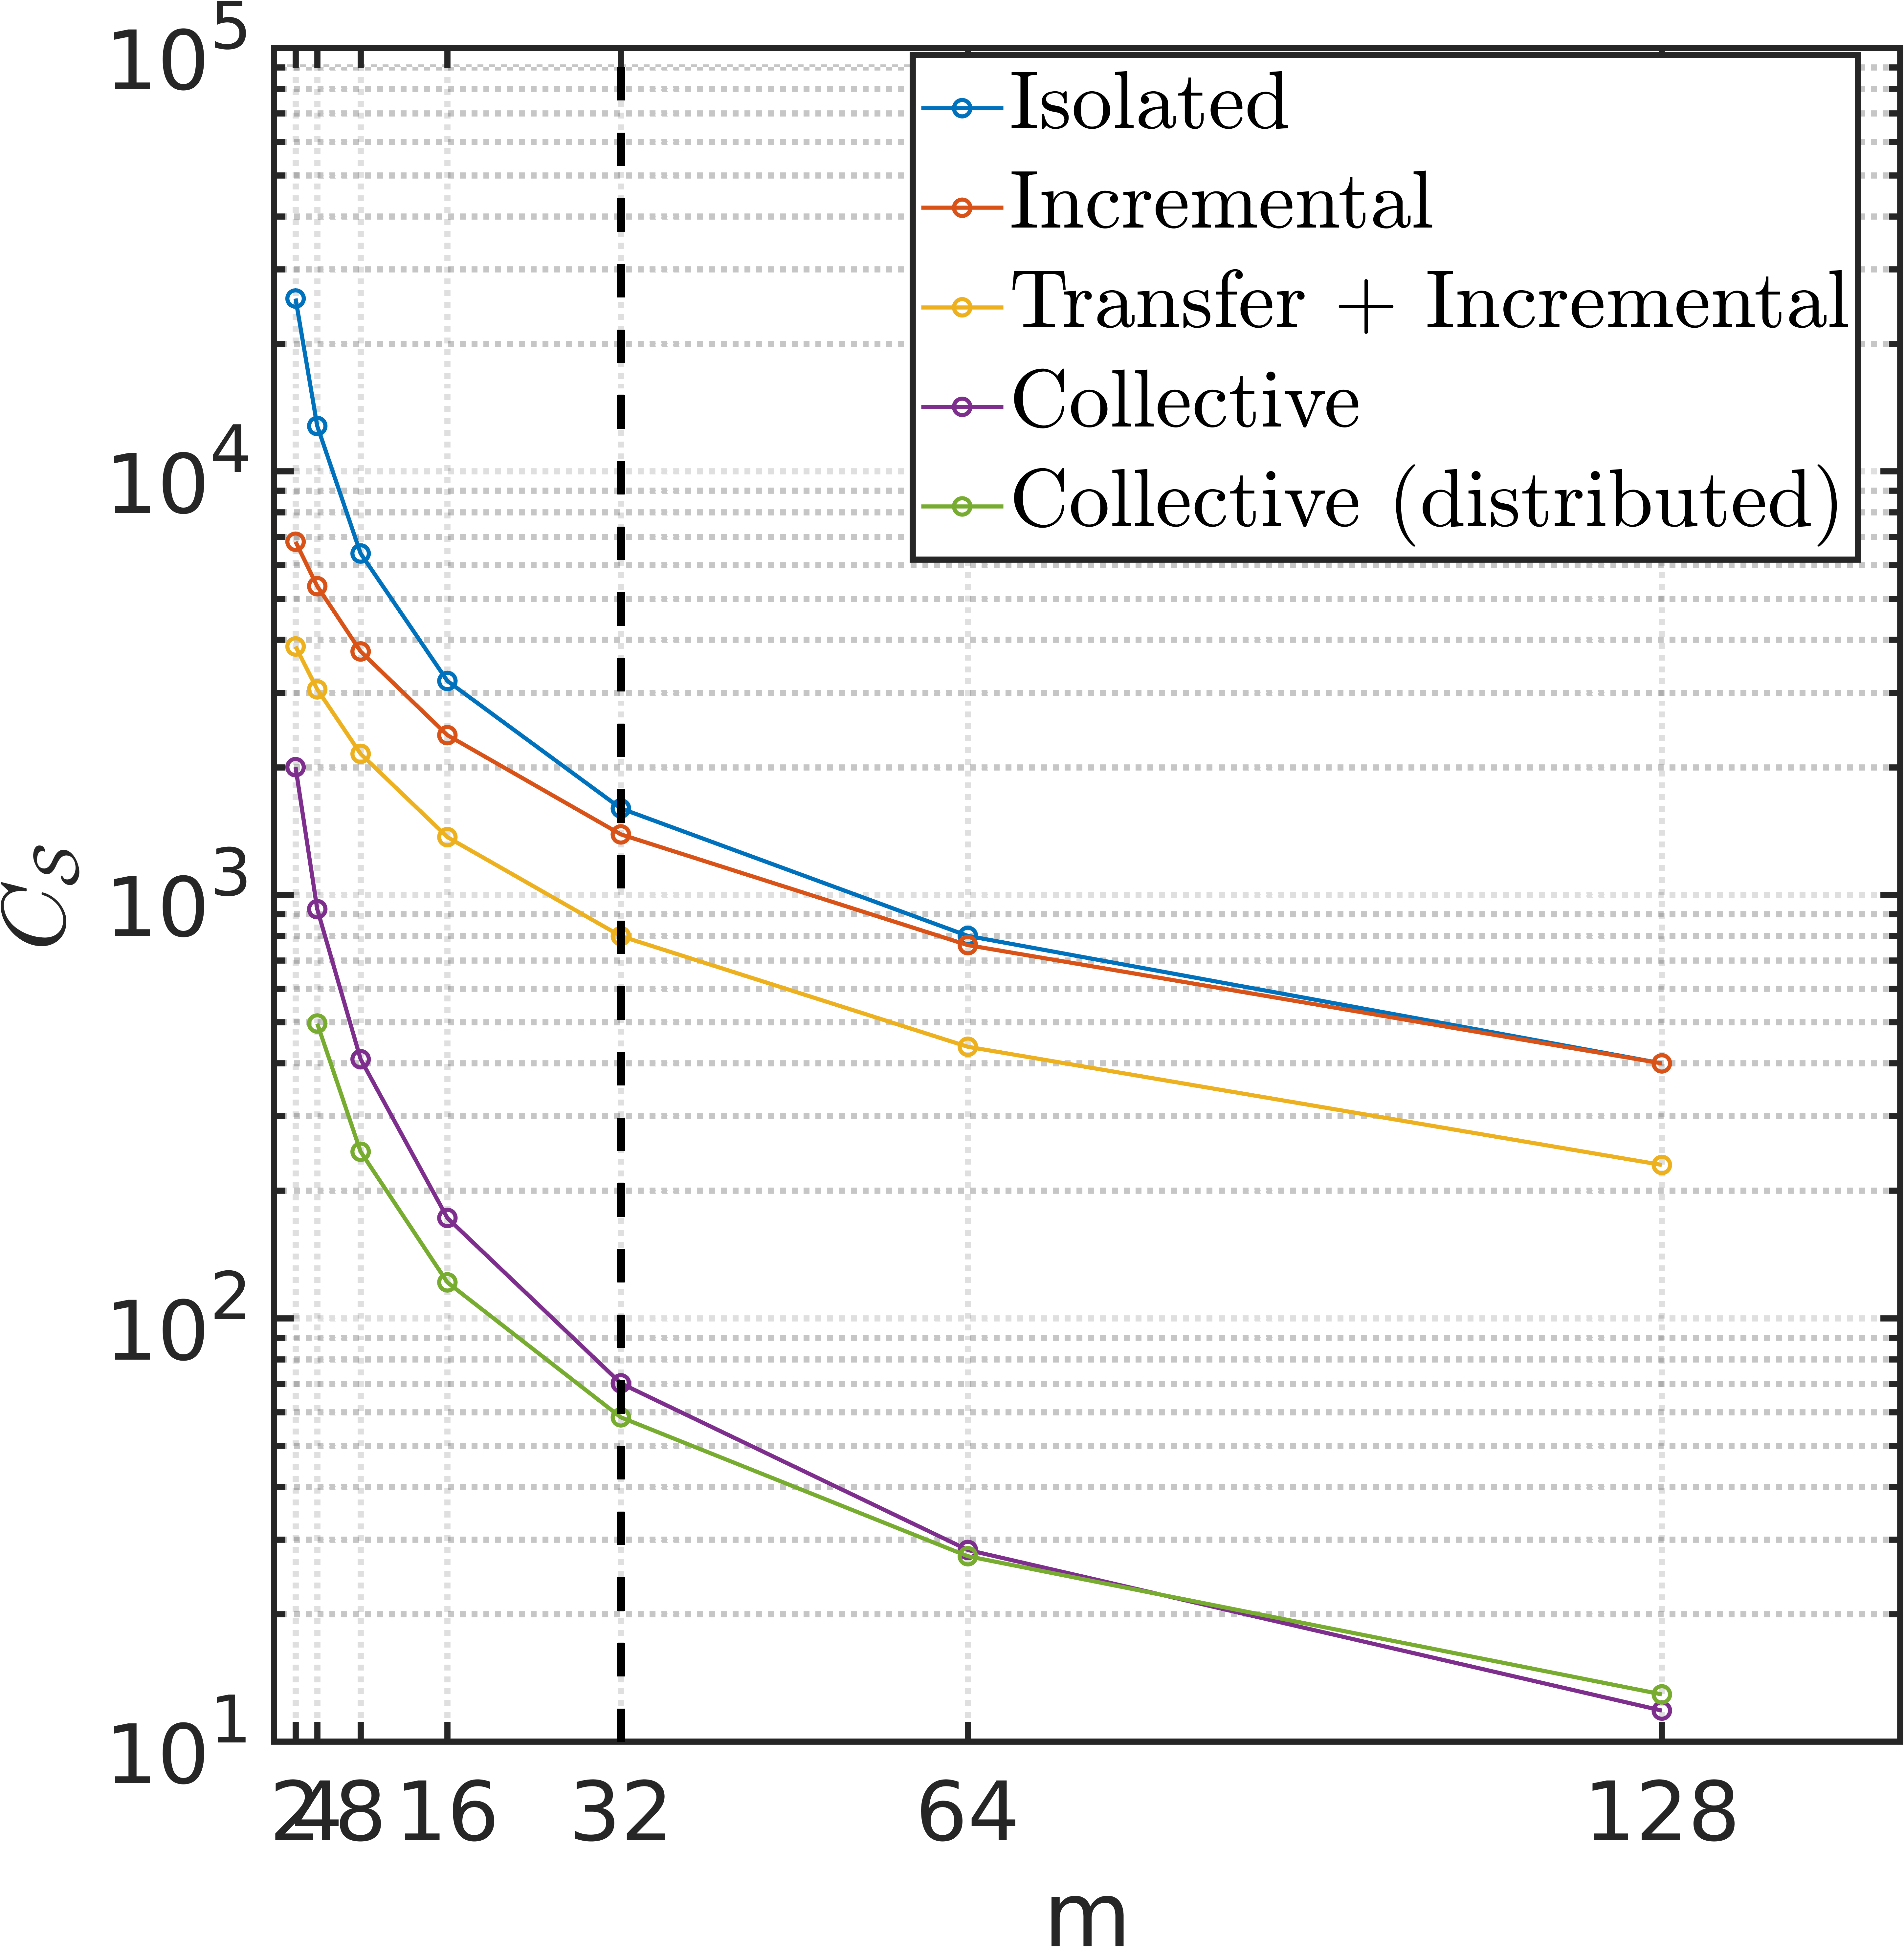
\includegraphics[width= \textwidth]{total_episodes_per_n_robots.png} \label{fig:total_episodes_per_n_robots}
%	\end{subfigure}
%	\hfill
%	\begin{subfigure}[t]{0.45\textwidth}
%		\subcaption{}
%		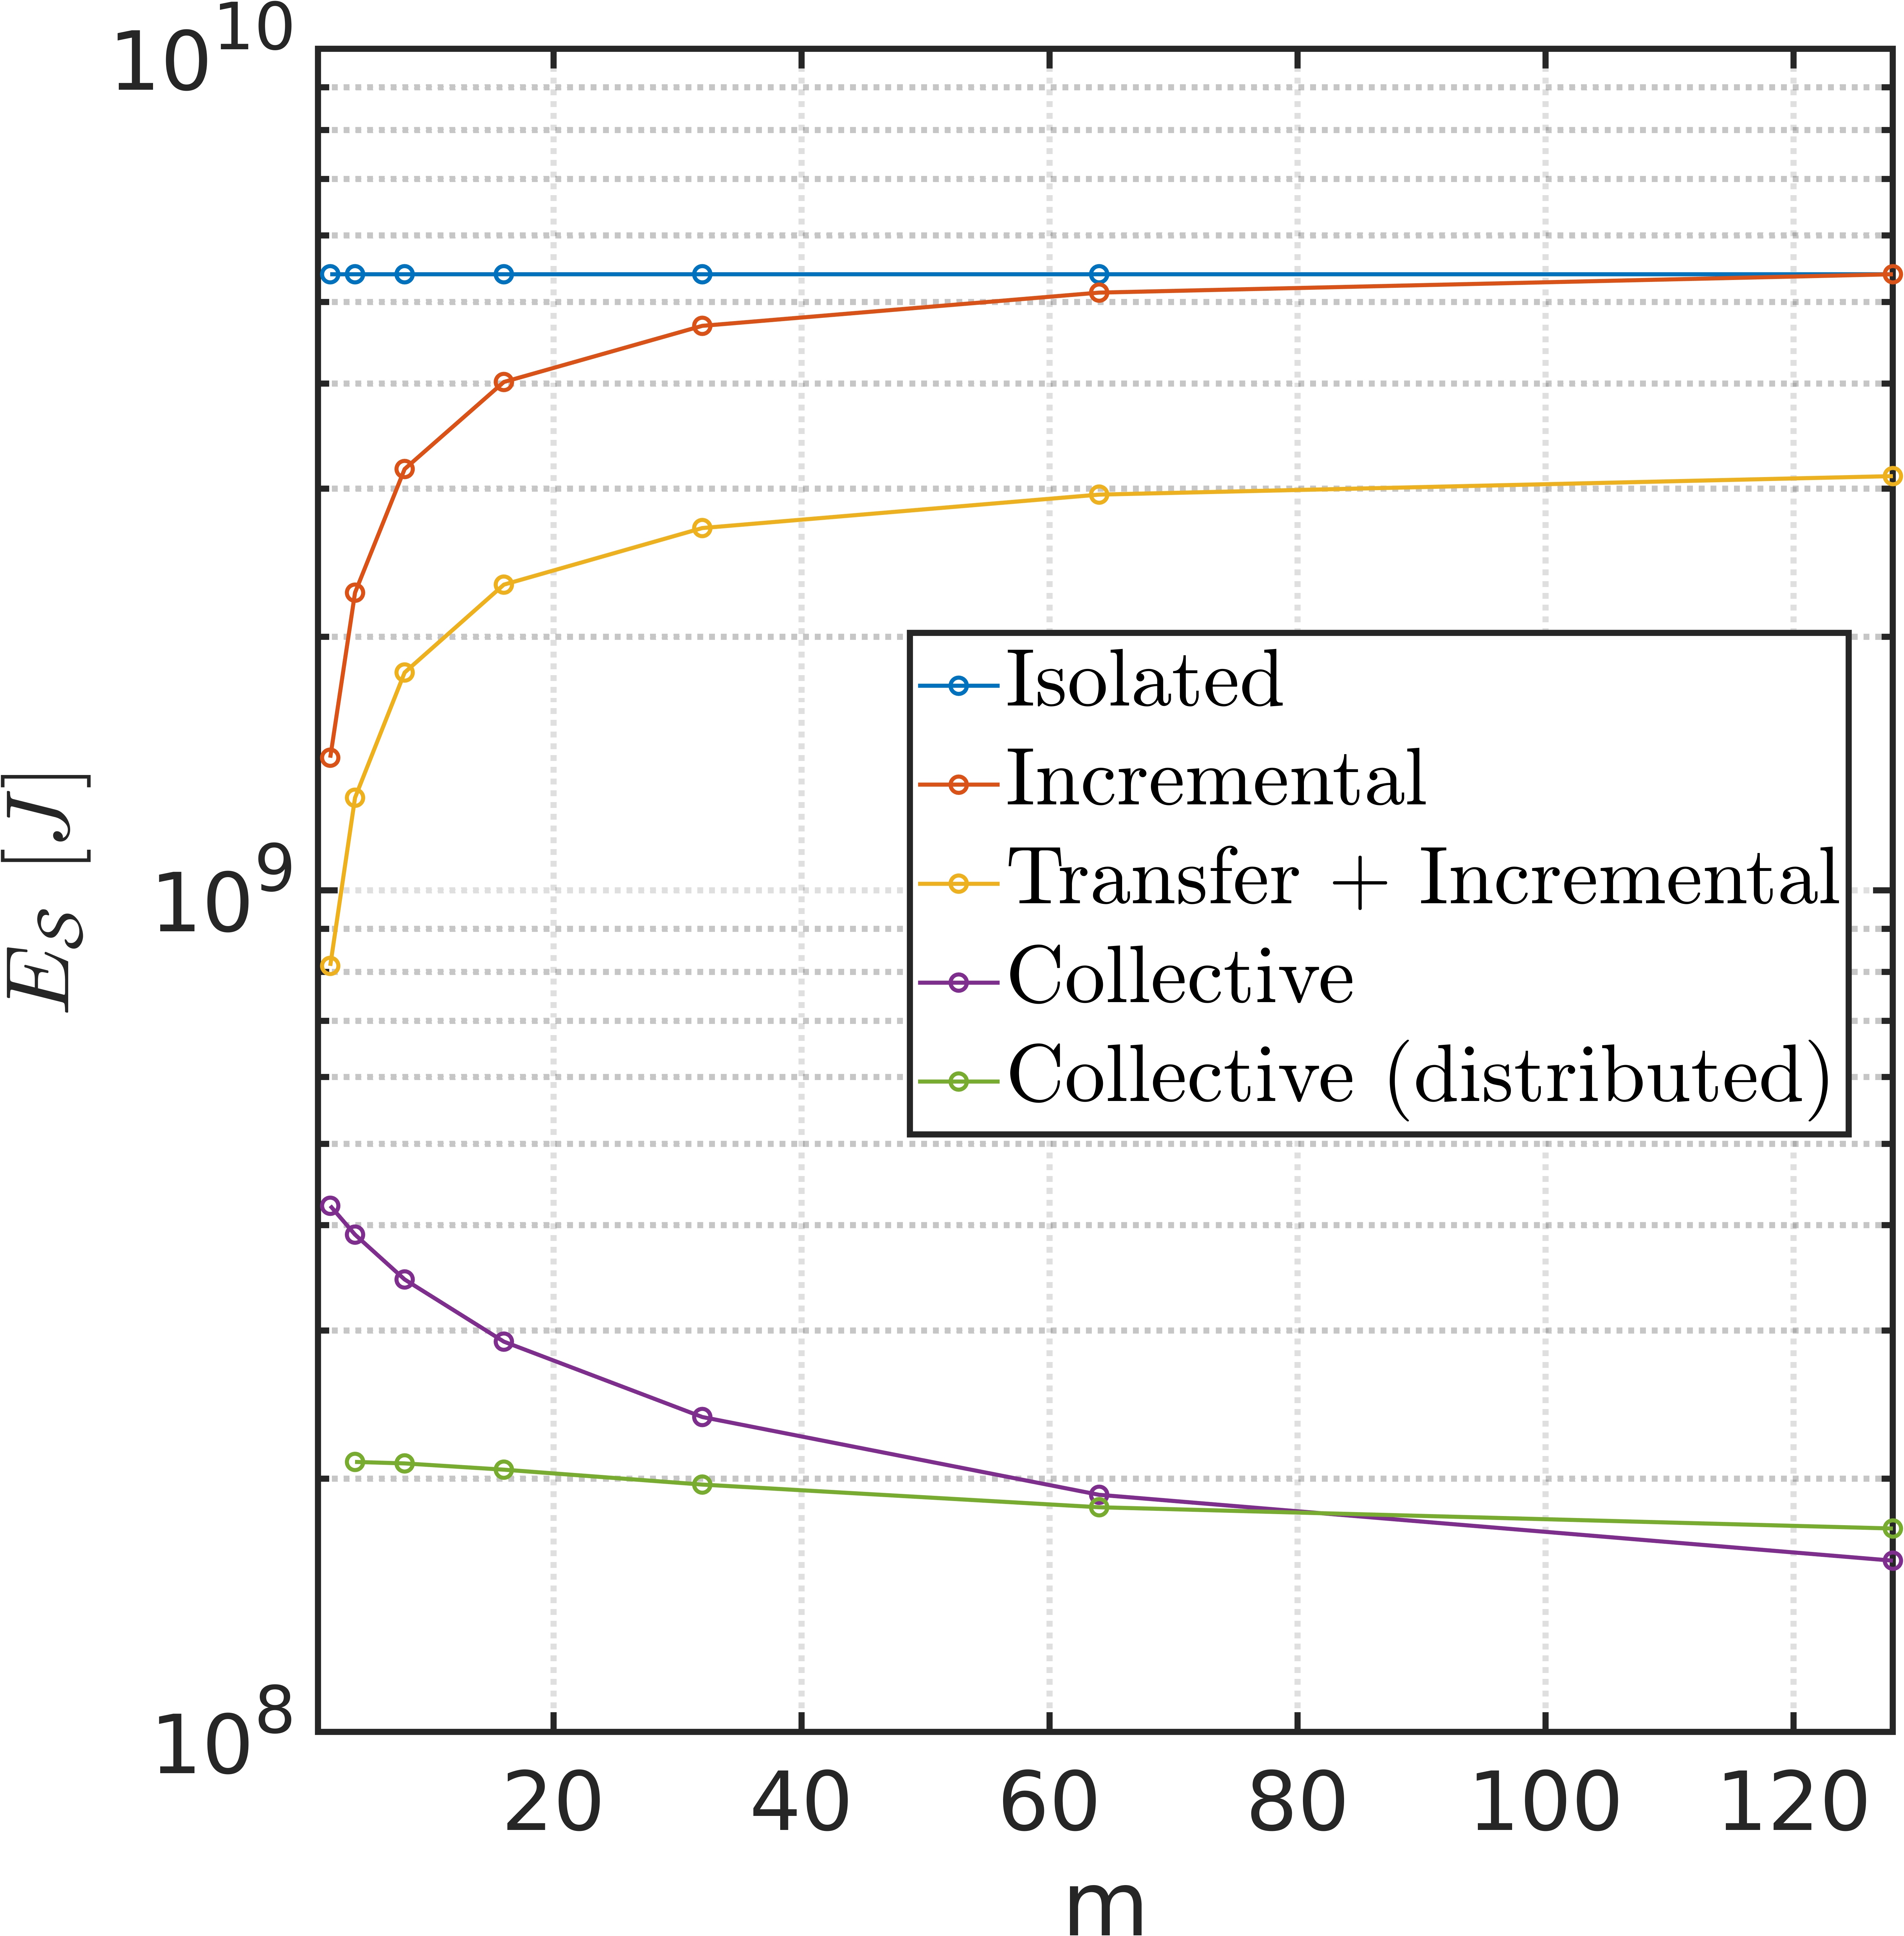
\includegraphics[width=\textwidth]{total_energy_per_n_robots.png} \label{fig:total_energy_per_n_robots}
%	\end{subfigure}
%	\hspace*{\fill}
%	\caption[] {\label{fig:final_results} \textbf{The effect of the number of robots.} (\subref{fig:total_episodes_per_n_robots}) Total number of episodes to learn the universe of skills as a function of the available robots and (\subref{fig:total_energy_per_n_robots}) the total energy consumption.}
%\end{figure*}
%% ---
% ---
\begin{figure*}[!t]
	\centering
	\hspace*{\fill}
	\begin{subfigure}[t]{0.45\textwidth}
		\subcaption{}
		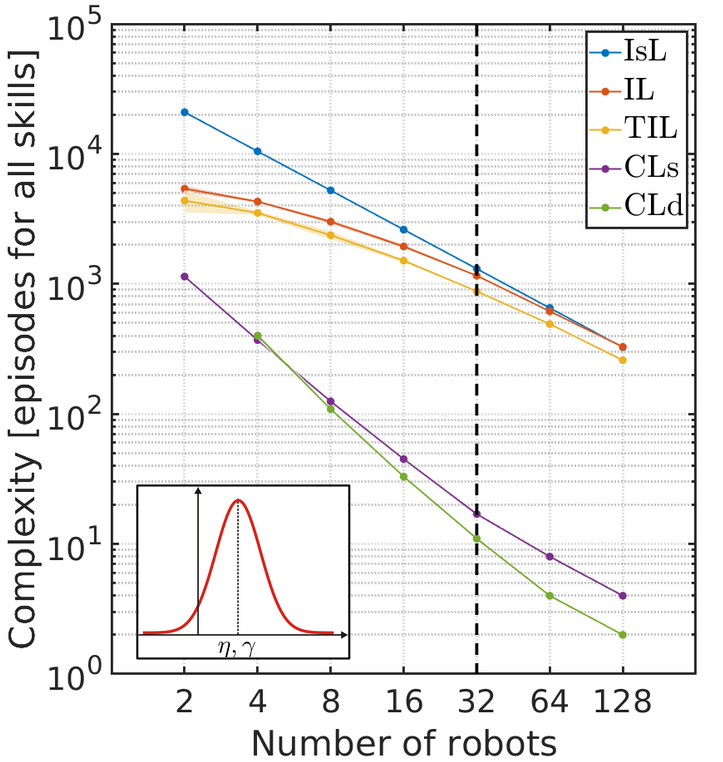
\includegraphics[width= \textwidth]{sf_learning_paradigms_complexity_tmp.png} \label{fig:total_episodes_per_n_robots}
	\end{subfigure}
	\hfill
	\begin{subfigure}[t]{0.45\textwidth}
		\subcaption{}
		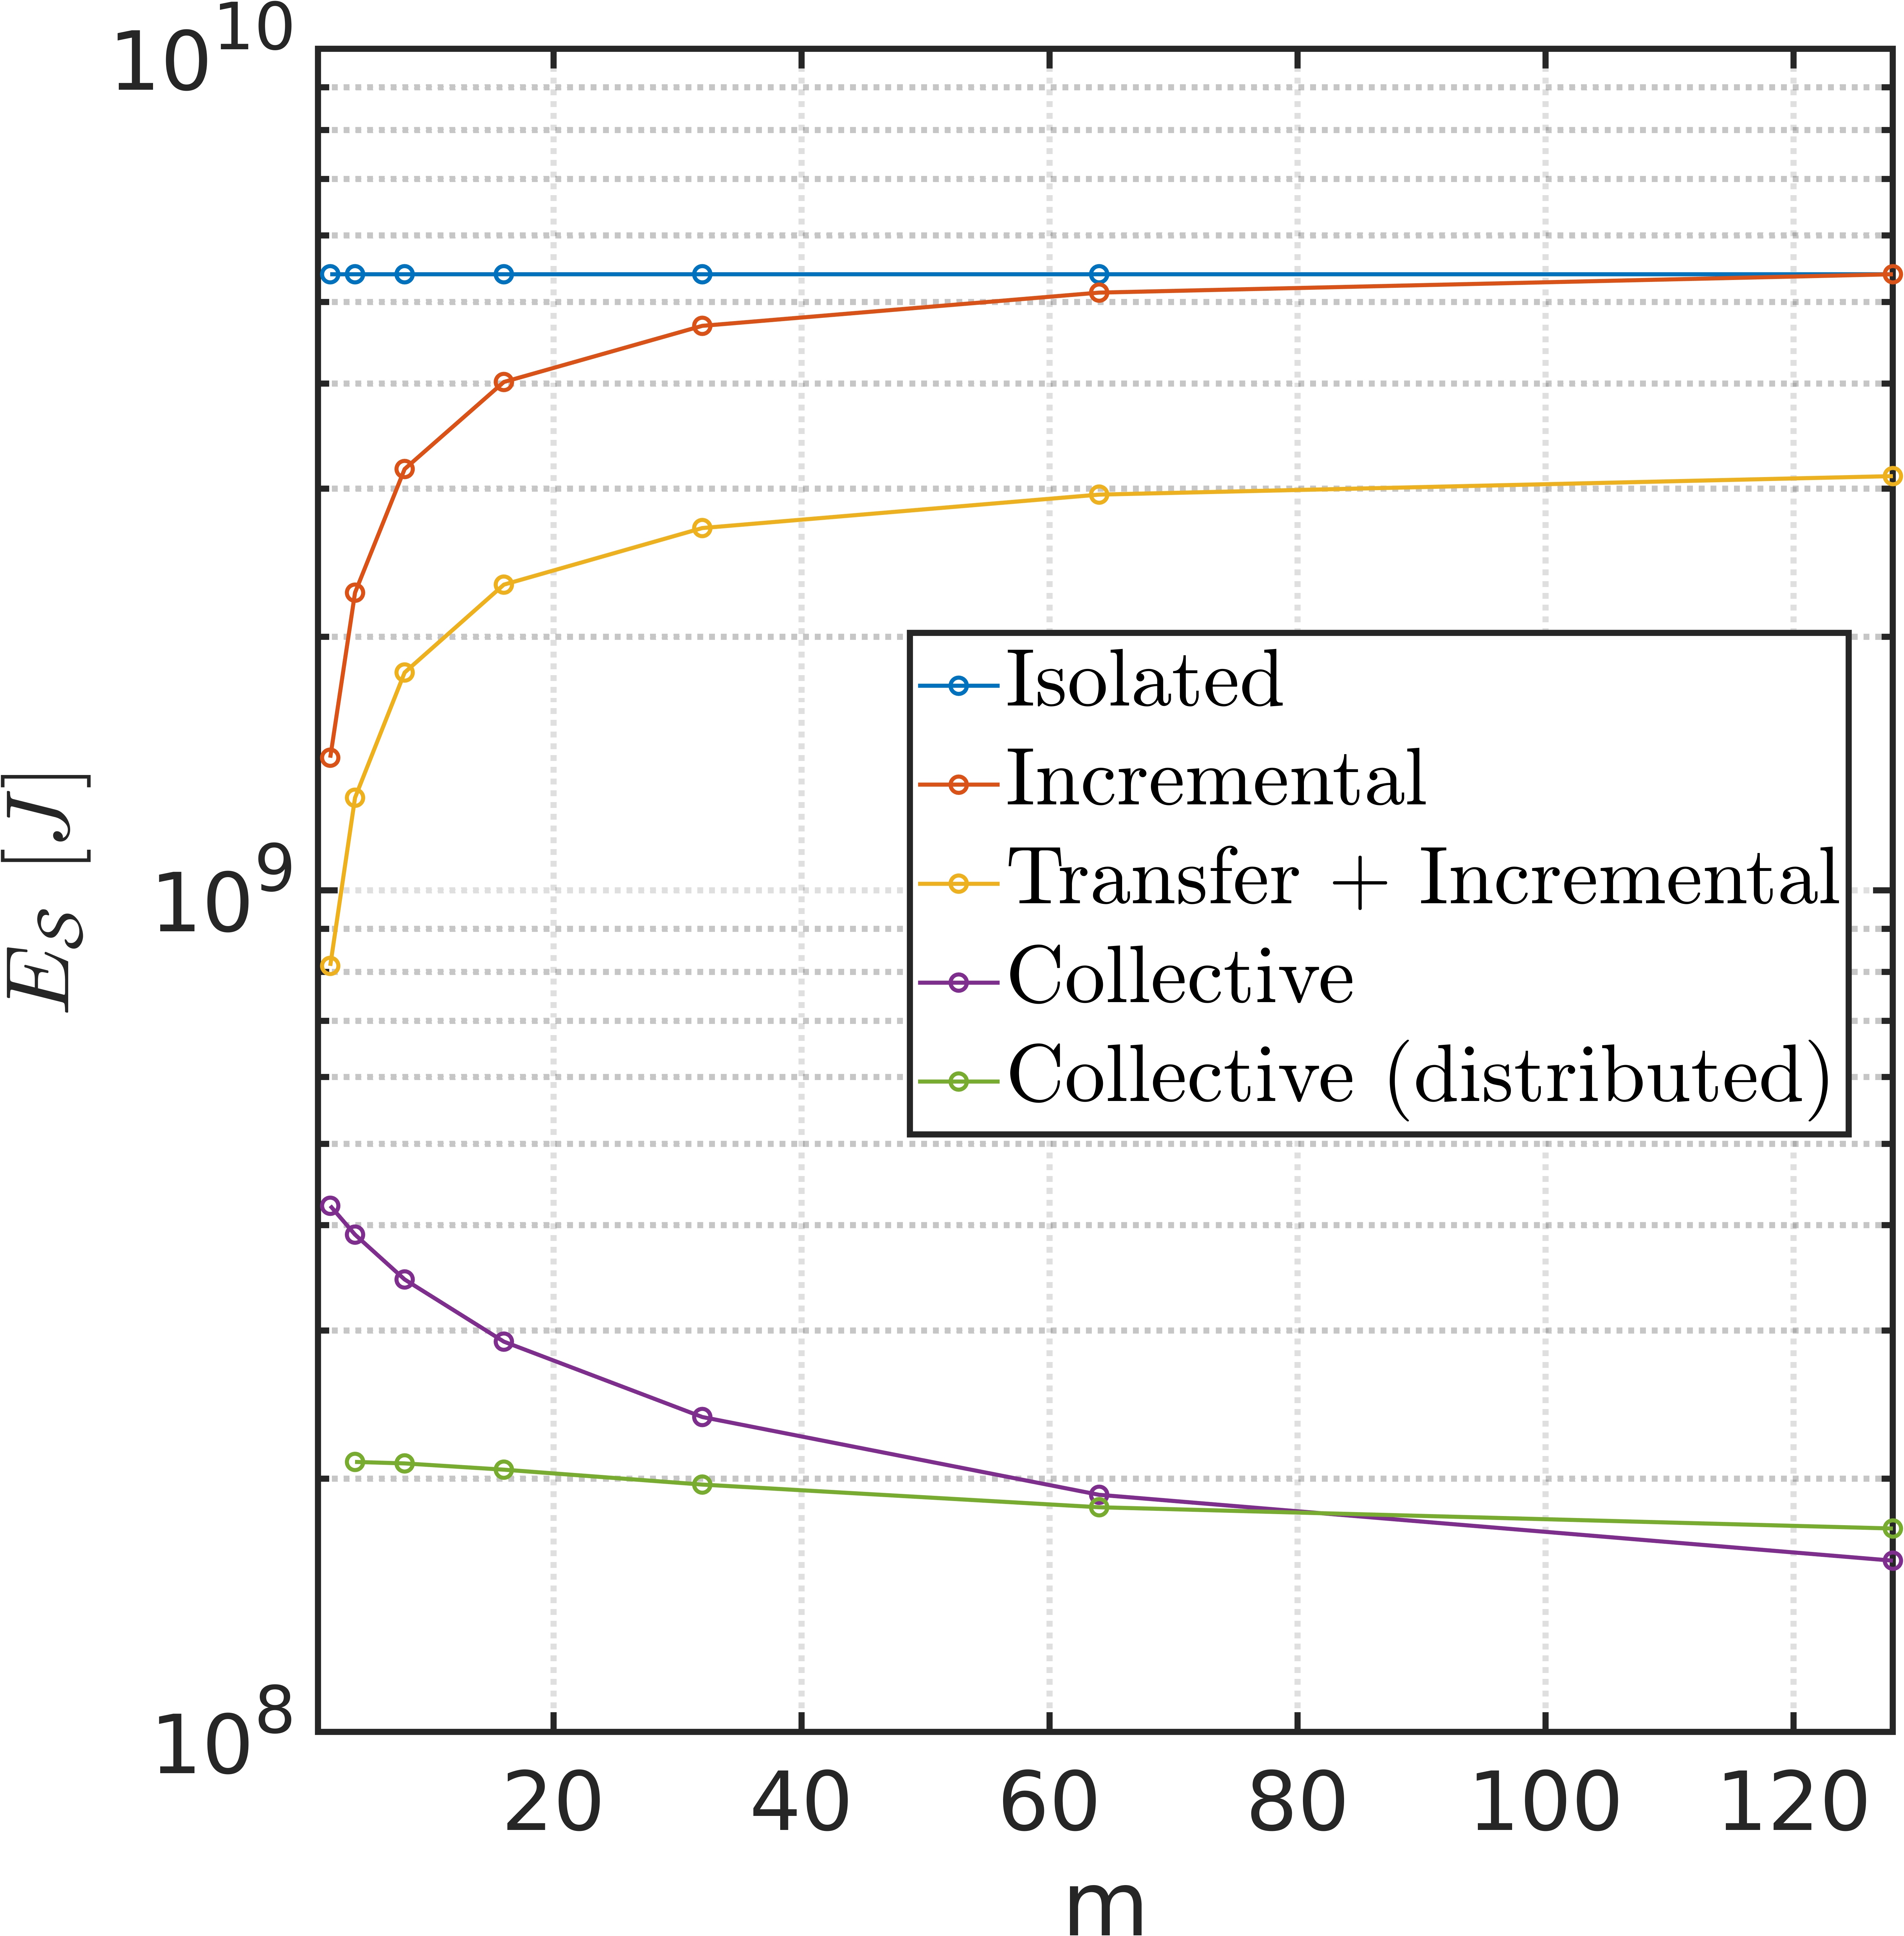
\includegraphics[width=\textwidth]{total_energy_per_n_robots.png} \label{fig:total_energy_per_n_robots}
	\end{subfigure}
	\hspace*{\fill}
	\caption[] {\label{fig:final_results} \textbf{The effect of the number of robots.} (\subref{fig:total_episodes_per_n_robots}) Total number of episodes to learn the universe of skills as a function of the available robots and (\subref{fig:total_energy_per_n_robots}) the total energy consumption.\pending{Replace with new figures}}
\end{figure*}
% ---

% SUBSECTION ========================================================================================
\paragraph*{Energy consumption}
The results in Fig.~\ref{fig:total_episodes_per_n_robots} show the total number of episodes required by each of the $m$ robots to learn the skills. To compute the total energy demand, those numbers need to be scaled by the factor $m e_0$, which leads to the consumption shown in Fig.~\ref{fig:total_energy_per_n_robots}. Undoubtedly, CL shows that it has not only the best energy usage of all the paradigms but, unlike the rest, the more robots take part in learning the universe of skills, the better overall energy usage.
% ---
\begin{figure*}[t!]
	\centering
	\hspace*{\fill}
	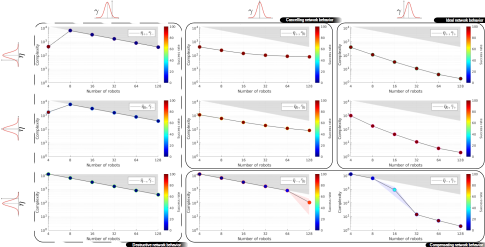
\includegraphics[width=\textwidth]{template_figure_dcl_cases.png}
	\hspace*{\fill}
	\caption[] {\label{fig:dcl_cases_matrix_tmp} \textbf{Total complexity of \ac{dcl} for different values of $\eta$ and $\gamma$.} \myhl{There exist nine possible combinations for the values of $\eta$ and $\gamma$. The success rate (i.e., the number of learned skills) is included.} \pending{Rethink this figure.}}
\end{figure*}
% ---

% SUBSECTION ========================================================================================
\paragraph*{Performance \acl{dcl}}
\myhl{Using the same case of the smart factory, focusing on the performance of \ac{dcl} provides interesting insights. For example, Fig.~\ref{fig:dcl_categories_matrix_tmp} shows a matrix of nine different behaviors identified by varying qualitatively the values of the tuple $(\eta,\gamma)$. Out of this cases, their performance indicates that the \emph{ideal agent-collective behavior} and the \emph{compensating behavior} are desired.}
% ---
\begin{figure*}[t!]
	\centering
	\hspace*{\fill}
	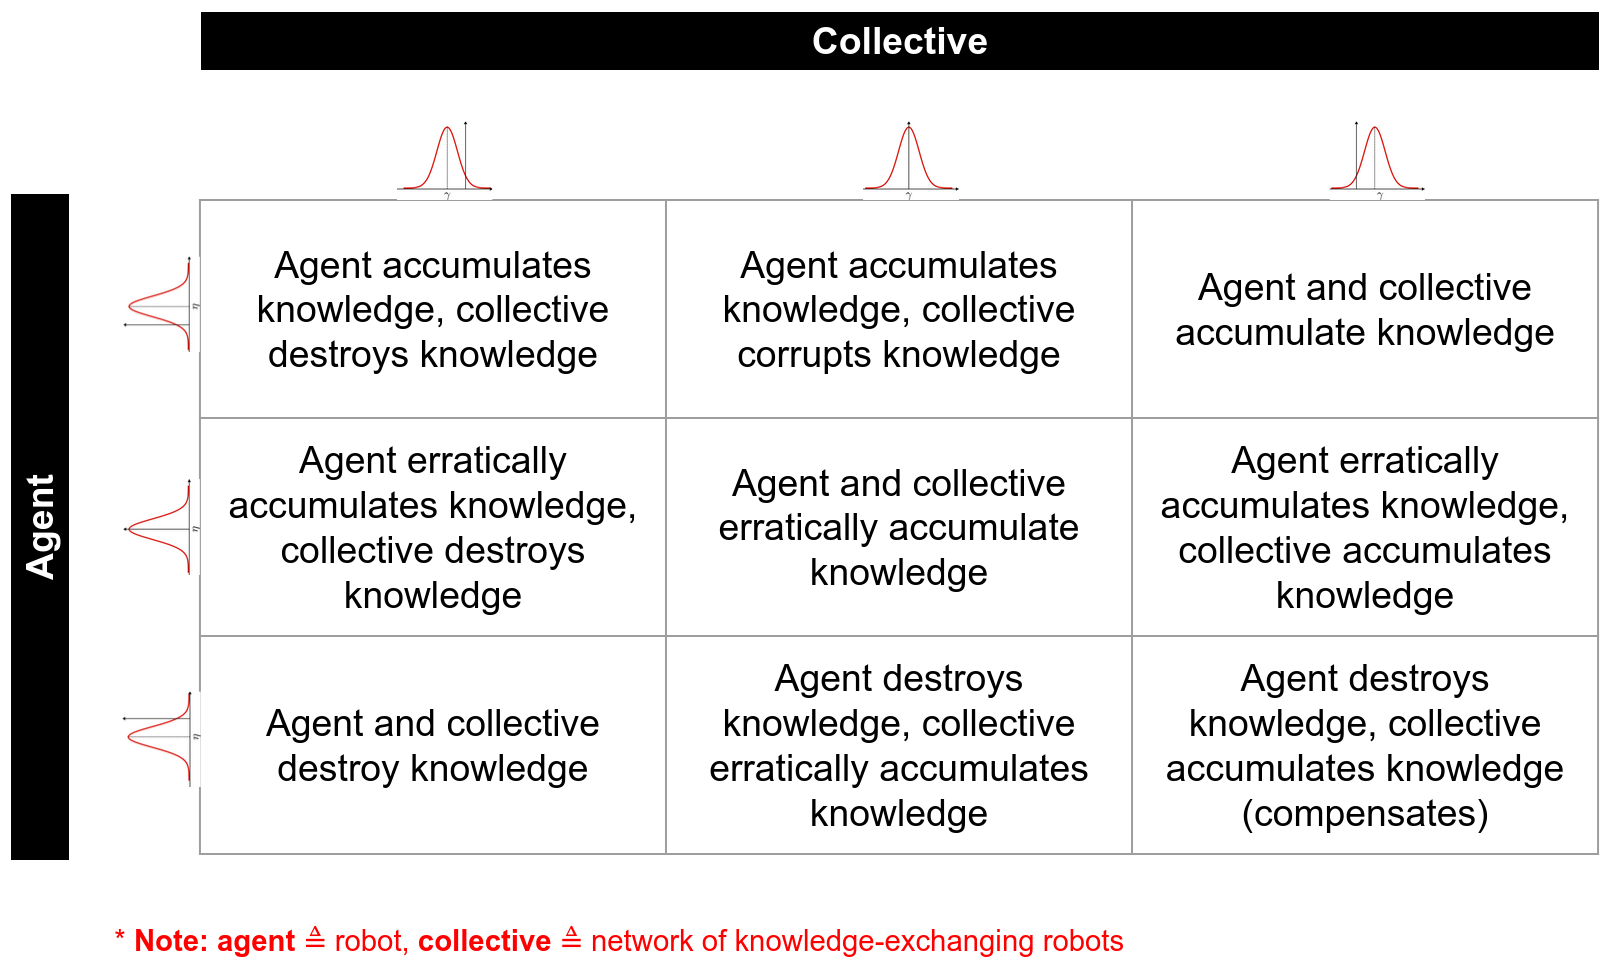
\includegraphics[width=14cm]{dcl_categories_matrix_tmp.png}
	\hspace*{\fill}
	\caption[] {\label{fig:dcl_categories_matrix_tmp} \textbf{Categorization of \ac{dcl} behavior.} \myhl{According to the values selected for $\eta$ and $\gamma$ in the \acl{dcl} scenario, nine general behaviors can be identified.} \pending{Rethink this figure.}}
\end{figure*}
% ---

% ===================================================================================================
%                                                 |                                                 |
%                                                 |                                                 |
% -------------------------------------------- SECTION ---------------------------------------------|
%                                                 |                                                 |
%                                                 |                                                 |
% ===================================================================================================
\section*{Discussion}\label{sec:discussion}
While the unprecedented strides in AI and robotics have revolutionized numerous sectors, the ongoing proliferation and associated energy consumption cannot be ignored. As the scope of AI continues to expand, a concerted effort is required to strike a balance between innovation and conscientious energy usage to steer AI toward sustainable operation. We introduced three principal energy expenditure categories to emphasize the significance of energy consumption in AI systems. We juxtaposed them with the grand challenges stemming from the escalating DAI applications and growing population of EAI agents. In particular, we underscored that mitigating energy consumption in EAI systems requires enhanced mechanical designs, efficient computation, and communication hardware, and a paramount emphasis on harnessing the simultaneous sharing, exchange, transfer, and accumulation of knowledge acquired by the various agents.

\myhl{The parameter $\alpha$ plays a crucial role in ensuring the robustness of both the model and its results, allowing the system to remain effective even across a wide range of embodiments. Despite these variations---primarily captured by $\alpha$---the idealized collective effect persists, provided that the inter-agent exchange factor $\gamma$ is chose sensible according to the stability conditions discussed in the \nameref{sec:supplementary_materials}. Given our assumptions, one of the most important and intriguing findings is the identification of regimes where \ac{cl} significantly outperforms the conventional learning paradigms. Notably, this advantageous regime appears to coincide with the parameter ranges expected in real-world scenarios, highlighting the significance of the collective knowledge sharing paradigm.}

\myhl{Various factors can influence the equations governing the system, including false communication, communication breaches, updates to the learning rate, and the correctness of transferred information. Each of these factors has the potential to alter key model parameters $(\alpha,\beta,\gamma,\eta)$, impacting overall system behavior. While the effects of embodiment distribution are primarily addressed by Assumptions~\ref{assumption:average_behavior} and \ref{assumption:agent_similarity}, the inter-agent exchange factor $\gamma$ can also serve as a means to model these variations.}

% ===================================================================================================
\paragraph*{Developing collective learning to address the energy challenges of EAI}
Fig.~\ref{fig:challengesConnected} depicts the natural connections between the energy grand challenges associated with EAI. This allows us to identify critical areas of opportunity for collective learning. Directly related to challenge C1 and the computation and communication energy expenditure ($E_\text{CCE}$), the EAI research community stands to gain significant headway by channeling efforts into realizing collective learning algorithms. This might involve focusing on data-efficient methodologies, infusing pertinent prior knowledge into models, or fostering knowledge-sharing capabilities. The latter emerges as an especially remarkable solution (as shown in our simulation study), poised to expedite multi-skill learning by leveraging a cloud-connected repository of skills. With time, this paradigm shift could transform data center demands from compute-intensive to storage and querying, drastically reducing energy needs, apart from the compelling need to advance computational algorithms to leverage efficient hardware and streamline communication protocols. Challenge C2 is intricately interwoven with the surging population of active robots and other intelligent machines. The relevance of better mechatronic designs (e.g., lightweight materials, flexible components, and energy-efficient actuation) for fine-tuning energy utilization during skill execution is obvious and a problem by itself. Collective learning can contribute to reducing the basal energy expenditure ($E_\text{BEE}$) and the energy implicated in motion and interaction ($E_\text{MIE}$) by reducing the time dedicated to learning and executing skills thanks to the body of knowledge collected by the multitude of agents with similar capabilities. Finally, the efforts devoted to approaching challenges C1 and C2 will ripple into advancements in C3. As mentioned before, recycling is a supplementary avenue for energy optimization in C3. Integrating recycling within the manufacturing landscape of machines would enable the reclamation of usable parts from retired robots and the reutilization of materials from discarded components. As the journey towards energy-efficient EAI unfolds, a holistic approach marrying innovative algorithms, efficient hardware, sustainable designs, and recycling endeavors offers promise.
% ---
\begin{figure}[!t]
	\centering
	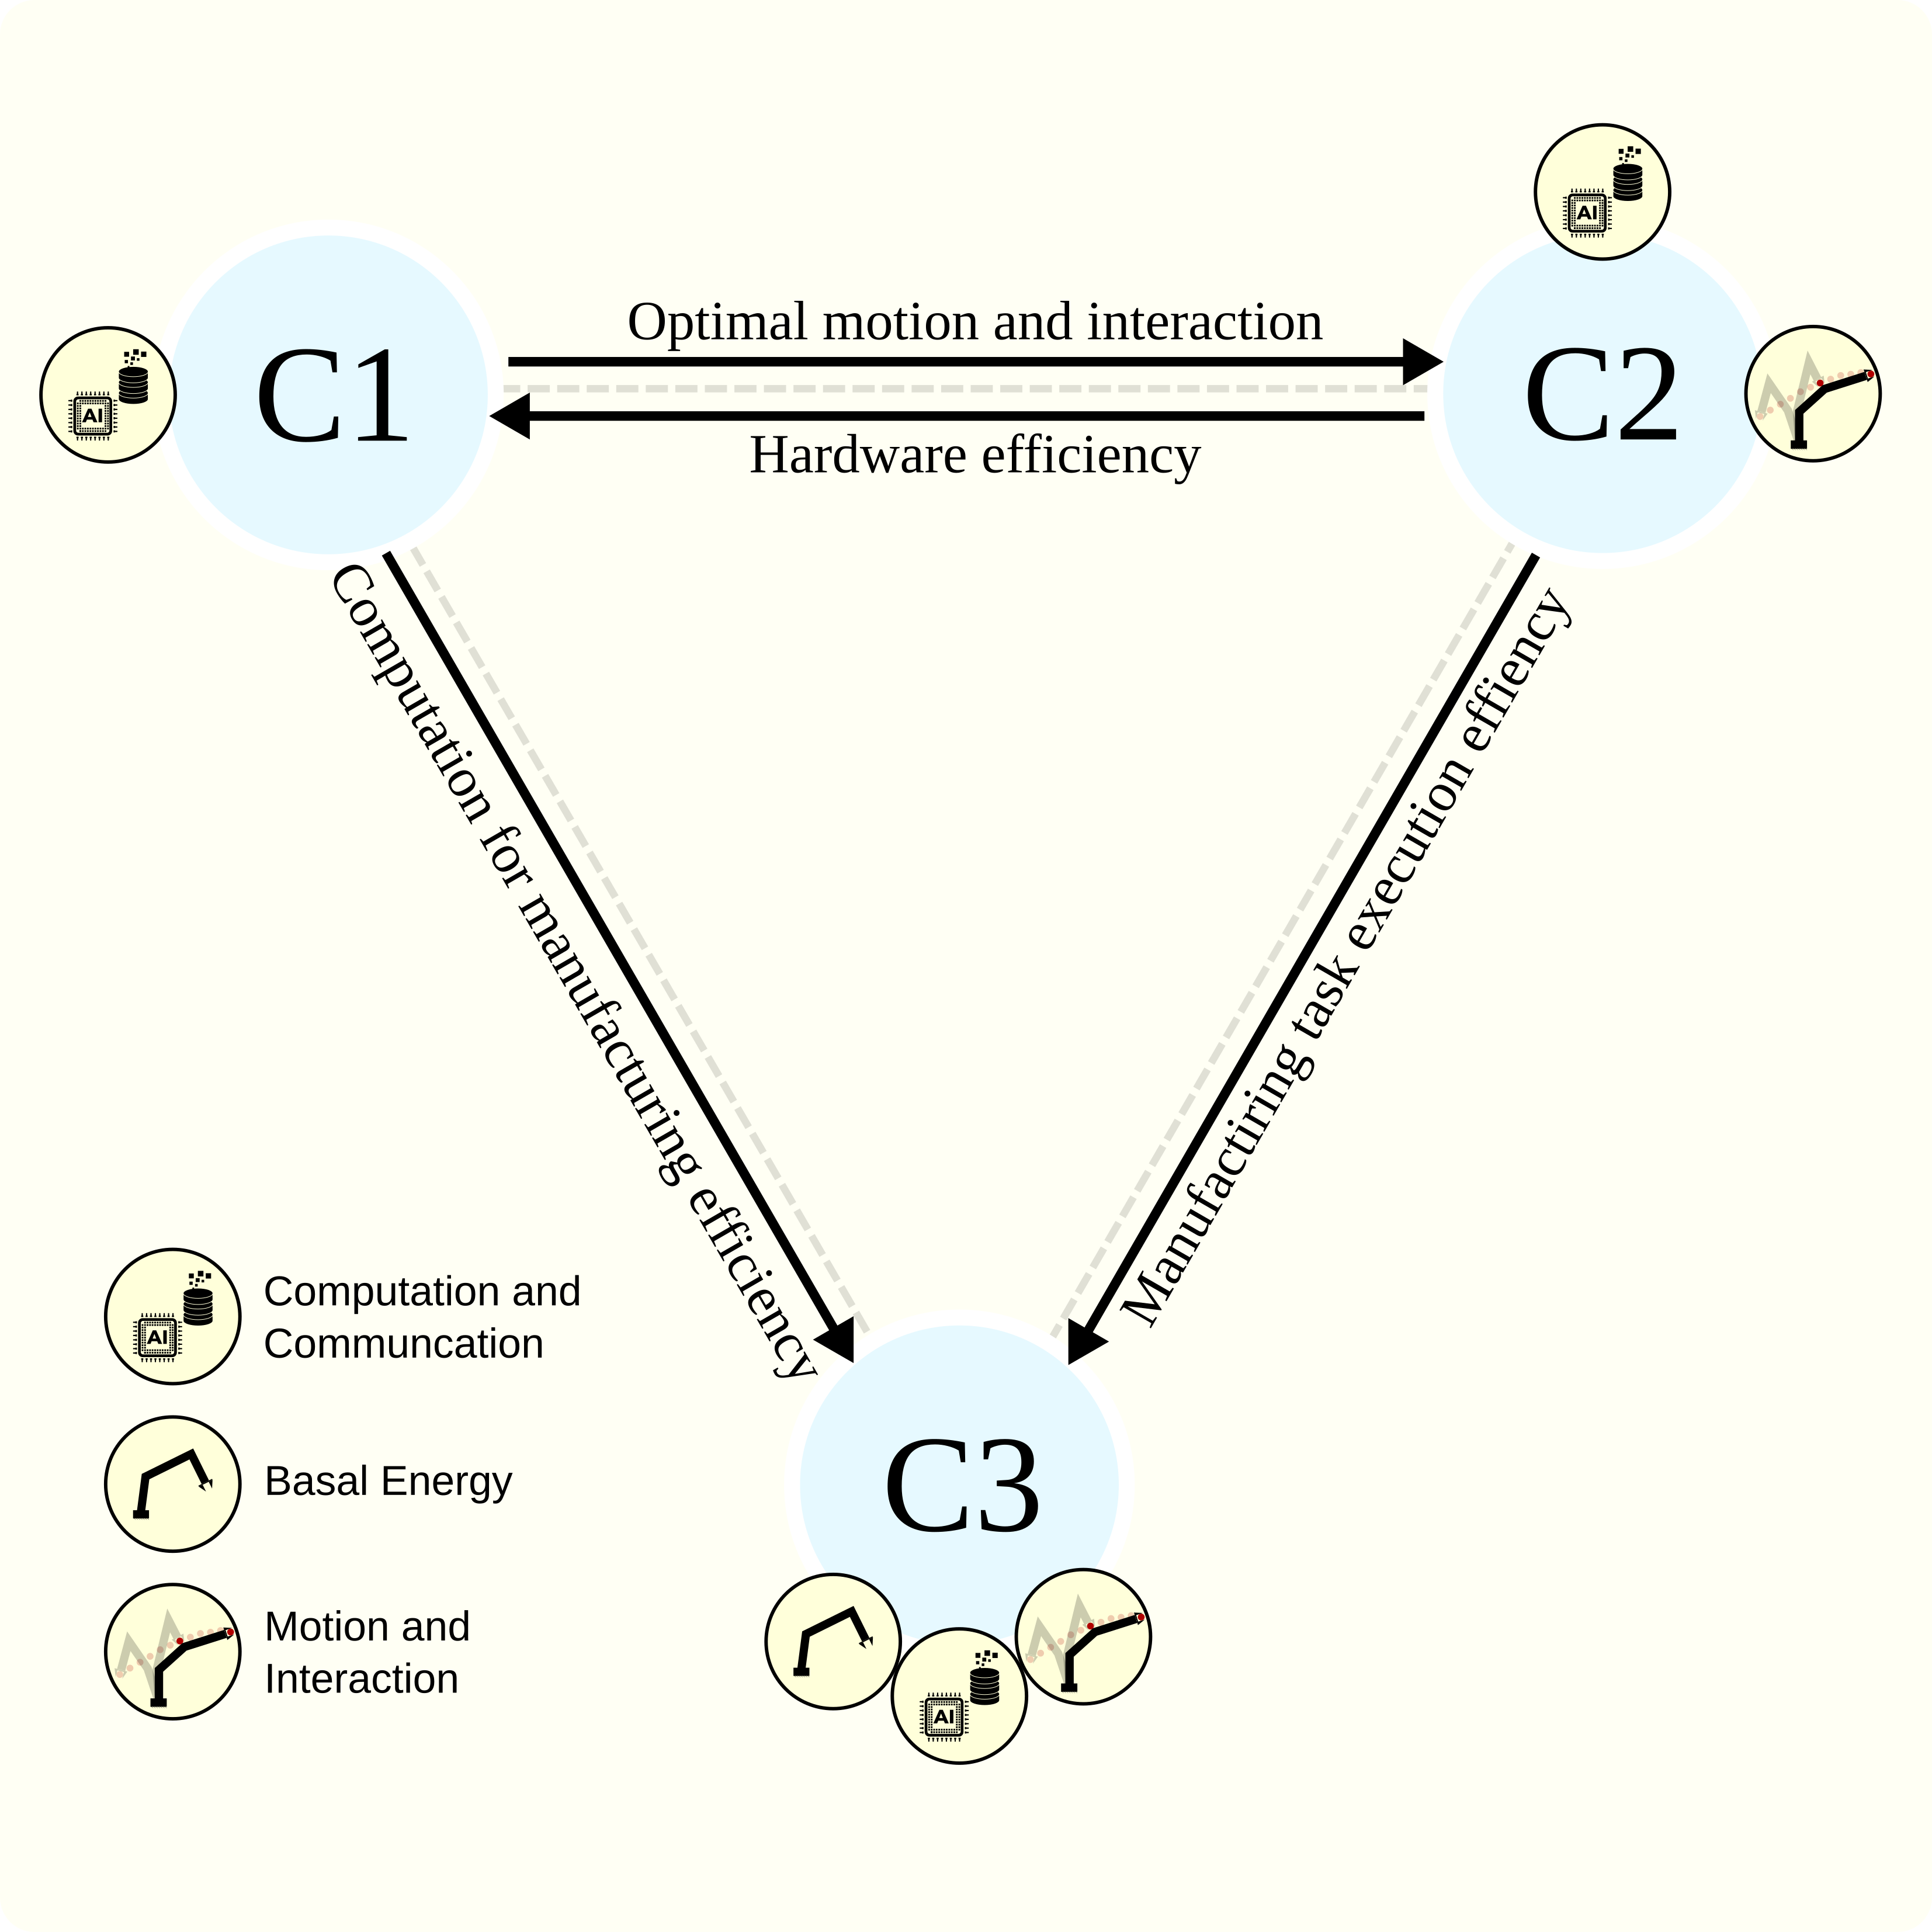
\includegraphics[width=0.45\textwidth]{fig/grand_challenges_connections.png}
	\caption{\textbf{Interconnection between challenges C1, C2, and C3.}}
	\label{fig:challengesConnected}
\end{figure}
% ---

% ===================================================================================================
\paragraph*{Closing remarks}
As discussed in \cite{Kaelbling2020foundationefficientrobot}, efficient robotic learning algorithms enabling agents to acquire new skills on the fly must possess specific key attributes: sample efficiency, generalizability, compositionality, and incremental learning capabilities. The CL paradigm inherently fulfills these prerequisites by harnessing the full communication potential of networked EAI agents. This approach facilitates real-time concurrent knowledge exchange and aggregation, resulting in energy- and time-efficient skill acquisition.

Our results suggest that utilizing the conventional paradigms of isolated, incremental, and transfer learning on many EAI agents does not lead to optimal energy utilization. This remains true even when multiple agents operate concurrently since, in the absence of true inter-agent knowledge exchange, energy requirements increase substantially as the number of EAI agents grows. Conversely, our simulation study highlighted that collective learning presents a solution to energy demands contingent on effectively sharing knowledge based on skill similarity. Notably, the CL paradigm showcased superior performance with increasing robot numbers, enabling concurrent acquisition of multiple skills.

While collective learning holds significant promise, it is crucial to recognize that the fundamental algorithms and infrastructure necessary to make it a reality are either nonexistent or in active development. Furthermore, contemporary state-of-the-art algorithms focusing on proper incremental and transfer learning are still in the early stages of development. However, although our primary focus has centered on how collective learning addresses the formidable energy challenges posed by EAI, it is essential to acknowledge that its potential extends far beyond this specific domain.

The collective learning paradigm is equally applicable to DAI agents. Indeed, recent developments have shed light on the potential of edge computing and federated learning, wherein computational tasks are distributed beyond the confines of centralized data centers to multiple DAI agents. Furthermore, foundational models developed through extensive research and learning now serve as cornerstones for solving more specific, nuanced tasks, remarking the power of true knowledge transfer.

Much like in the context of EAI, the promise of collective learning for DAI becomes evident if efficient means to exchange and aggregate knowledge from DAI agents, each running its learning routines, are established. The synergies facilitated by the CL approach have the potential to significantly enhance the problem-solving capabilities and energy efficiency of DAI applications. This ultimately underscores the versatility and potential impact of collective learning across the spectrum of artificial intelligence domains. We hope the arguments in this discussion catalyze further research endeavors, ultimately bringing collective learning to fruition.

% ===================================================================================================
%                                                 |                                                 |
%                                                 |                                                 |
% -------------------------------------------- SECTION ---------------------------------------------|
%                                                 |                                                 |
%                                                 |                                                 |
% ===================================================================================================
\section*{Supplementary Materials}
Sections \ref{sec:materials_and_methods} to \ref{sec:app_robot_ener_consumption}\\
Fig.~\ref{fig:power_per_episode} to Fig.~\ref{fig:cobot_watt_per_kg}

% ===================================================================================================
%                                                 |                                                 |
%                                                 |                                                 |
% -------------------------------------------- SECTION ---------------------------------------------|
%                                                 |                                                 |
%                                                 |                                                 |
% ===================================================================================================
\renewcommand\refname{References and Notes}
\bibliography{bib/References.bib}
\bibliographystyle{Science}

%\begin{thebibliography}{10}
%	
%	\bibitem{Szczepanski2019Economicimpactsartificial}
%	M.~Szczepanski, Economic impacts of artificial intelligence ({AI}) (2019).
%	
%	\bibitem{Strubell2019EnergyPolicyConsiderations}
%	E.~Strubell, A.~Ganesh, A.~McCallum, {\it Energy and Policy Considerations for
%		Deep Learning in NLP\/}, {\it ACL\/} (2019).
%	
%	\bibitem{Cao2020TowardsAccurateReliable}
%	Q.~Cao, A.~Balasubramanian, N.~Balasubramanian, {\it Towards Accurate and
%		Reliable Energy Measurement of {NLP} Models\/}, {\it Proceedings of
%		SustaiNLP: Workshop on Simple and Efficient Natural Language Processing\/}
%	(Association for Computational Linguistics, Online, 2020), pp. 141--148.
%	
%	\bibitem{Chebotar2019Closingsimreal}
%	Y.~Chebotar, {\it et~al.\/}, {\it Closing the sim-to-real loop: Adapting
%		simulation randomization with real world experience\/}, {\it 2019
%		International Conference on Robotics and Automation (ICRA)\/} (IEEE, 2019),
%	pp. 8973--8979.
%	
%	\bibitem{Lehdonvirta2022futuresunpaidwork}
%	V.~Lehdonvirta, L.~P. Shi, E.~Hertog, N.~Nagase, Y.~Ohta, {\it The future (s)
%		of unpaid work: How susceptible do experts from different backgrounds think
%		the domestic sphere is to automation?\/}, {\it Plos one\/} {\bf 18}, e0281282
%	(2023).
%	
%	\bibitem{andrae2015global}
%	A.~S. Andrae, T.~Edler, {\it On global electricity usage of communication
%		technology: trends to 2030\/}, {\it Challenges\/} {\bf 6}, 117 (2015).
%	
%	\bibitem{Hintemann2022Cloudcomputingdrives}
%	R.~Hintemann, S.~Hinterholzer, Cloud computing drives the growth of the data
%	center industry and its energy consumption (2022).
%	
%	\bibitem{schwartz2019green}
%	R.~Schwartz, J.~Dodge, N.~A. Smith, O.~Etzioni, Green ai (2019).
%	
%	\bibitem{vinuesa2020role}
%	R.~Vinuesa, {\it et~al.\/}, {\it The role of artificial intelligence in
%		achieving the {S}ustainable {D}evelopment {G}oals\/}, {\it Nature
%		Communications\/} {\bf 11}, 1 (2020).
%	
%	\bibitem{zhou2020hulk}
%	X.~Zhou, Z.~Chen, X.~Jin, W.~Y. Wang, {\it HULK: An Energy Efficiency Benchmark
%		Platform for Responsible Natural Language Processing\/}, {\it arXiv preprint
%		arXiv:2002.05829\/}  (2020).
%	
%	\bibitem{Dalgren2019GreenMLA}
%	A.~Dalgren, Y.~Lundeg{\aa}rd, {\it GreenML : A methodology for fair evaluation
%		of machine learning algorithms with respect to resource consumption\/}
%	(2019).
%	
%	\bibitem{GarciaMartin2019Estimationenergyconsumption}
%	E.~Garc{\'\i}a-Mart{\'\i}n, C.~F. Rodrigues, G.~Riley, H.~Grahn, {\it
%		Estimation of energy consumption in machine learning\/}, {\it Journal of
%		Parallel and Distributed Computing\/} {\bf 134}, 75 (2019).
%	
%	\bibitem{real2019regularized}
%	E.~Real, A.~Aggarwal, Y.~Huang, Q.~V. Le, {\it Regularized evolution for image
%		classifier architecture search\/}, {\it Proceedings of the aaai conference on
%		artificial intelligence\/} (2019), pp. 4780--4789.
%	
%	\bibitem{krizhevsky2012imagenet}
%	A.~Krizhevsky, I.~Sutskever, G.~E. Hinton, {\it Imagenet classification with
%		deep convolutional neural networks\/}, {\it Advances in neural information
%		processing systems\/} {\bf 25}, 1097 (2012).
%	
%	\bibitem{IFR2019}
%	{\relax International Federation of Robotics}, {\it World Robotics 2019
%		Industrial Robots\/} (IFR Statistical Department, 2019).
%	
%	\bibitem{sirkin2015}
%	H.~L. Sirkin, M.~Zinser, J.~Rose, How robots will redefine competitiveness
%	(2015). Retrieved March 8, 2016 from: \url{https://goo.gl/YxPfyF}.
%	
%	\bibitem{fraunhofer2016}
%	{\relax Fraunhofer ISE}, Net installed electricity generation capacity in
%	germany. Retrieved March 9, 2016 from:
%	\url{https://www.energy-charts.de/power_inst.htm}.
%	
%	\bibitem{tobe2015}
%	F.~Tobe, Why cobots will be a huge innovation and growth driver for robotics
%	industry (2015). Retrieved April 5, 2016 from: \url{http://goo.gl/hRG5Du}.
%	
%	\bibitem{IFR2015}
%	{\relax International Federation of Robotics}, Service robot statistics.
%	Retrieved April 5, 2016 from:
%	\url{http://www.ifr.org/service-robots/statistics/}.
%	
%	\bibitem{schroder2014}
%	S.~Schr\"oder, Optimized movements: Ballet of the bots (2014). Retrieved March
%	8, 2016 from: \url{http://goo.gl/0Ir231}.
%	
%	\bibitem{CUT2015Smoothrobotmovements}
%	{\relax Chalmers University of Technology}, Smooth robot movements reduce
%	energy consumption by up to 40 percent (2015). Retrieved March 8, 2016 from:
%	\url{www.sciencedaily.com/releases/2015/08/150824064923.htm}.
%	
%	\bibitem{Mohammed2014MinimizingEnergyConsumption}
%	A.~Mohammed, B.~Schmidt, L.~Wang, L.~Gao, {\it Minimizing Energy Consumption
%		for Robot Arm Movement\/}, {\it Procedia CIRP\/} {\bf 25}, 400 (2014).
%	
%	\bibitem{Chemnitz2011Analyzingenergyconsumption}
%	M.~Chemnitz, G.~Schreck, J.~Krüger, {\it Analyzing energy consumption of
%		industrial robots\/}, {\it Emerging Technologies Factory Automation (ETFA),
%		2011 IEEE 16th Conference on\/} (2011), pp. 1--4.
%	
%	\bibitem{Haddadin2014SystemzumErstellen}
%	S.~Haddadin, System zum erstellen von steuerungsdatens\"atzen f\"ur roboter
%	(2014). German Patent {DE} 10 2014 112 639 B4 2018.02.08.
%	
%	\bibitem{Haddadin2015Systemgeneratingsets}
%	S.~Haddadin, System for generating sets of control data for robots (2015).
%	European Patent {EP} 3 189 385 {B}1.
%	
%	\bibitem{Garavan2012CollectiveLearning}
%	T.~N. Garavan, R.~Carbery, {\it Collective Learning\/} (Springer US, Boston,
%	MA, 2012), pp. 646--649.
%	
%	\bibitem{levine2018learning}
%	S.~Levine, P.~Pastor, A.~Krizhevsky, J.~Ibarz, D.~Quillen, {\it Learning
%		hand-eye coordination for robotic grasping with deep learning and large-scale
%		data collection\/}, {\it The International journal of robotics research\/}
%	{\bf 37}, 421 (2018).
%	
%	\bibitem{rudin2022learning}
%	N.~Rudin, D.~Hoeller, P.~Reist, M.~Hutter, {\it Learning to walk in minutes
%		using massively parallel deep reinforcement learning\/}, {\it Conference on
%		Robot Learning\/} (PMLR, 2022), pp. 91--100.
%	
%	\bibitem{flairop2023}
%	K.~I. f\"ur Technologie, {FLAIROP: Federated Learning for Robotic Picking},
%	\url{https://flairop.com/} (2023).
%	
%	\bibitem{Kaelbling2020foundationefficientrobot}
%	L.~P. Kaelbling, {\it The foundation of efficient robot learning\/}, {\it
%		Science\/} {\bf 369}, 915 (2020).
%	
%	\bibitem{statista_ir_cobot_share}
%	Statista, Share of traditional and collaborative robot unit sales worldwide
%	from 2018 to 2022 (2020).
%	
%	\bibitem{montaqim2015}
%	A.~Montaqim, Top 9 industrial robot companies and how many robots they have
%	around the world (2015). Retrieved March 8, 2016 from:
%	\url{http://goo.gl/QEIBr2}.
%	
%	\bibitem{fanuc2015}
%	{\relax FANUC America}, Fanuc announces record-breaking 400,000 robots sold
%	worldwide (2015). Retrieved March 8, 2016 from:
%	\url{http://www.fanucamerica.com/FanucAmerica-news/Press-releases/PressReleaseDetails.aspx?id=76}.
%	
%	\bibitem{yaskawa2014}
%	{\relax Motoman}, 7 things you may not know about yaskawa (2014). Retrieved
%	March 8, 2016 from:
%	\url{http://www.motoman.com/blog/index.php/7-things-may-know-yaskawa/}.
%	
%	\bibitem{ABB2015}
%	{\relax ABB}, {ABB Robotics} (2015). Retrieved March 8, 2016 from:
%	\url{http://new.abb.com/products/robotics}.
%	
%	\bibitem{statista_ir_operational_stock}
%	Statista, Operational stock of multipurpose industrial robots worldwide from
%	2010 to 2020 (2023).
%	
%	\bibitem{Heredia2023BreakingEnergyConsumption}
%	J.~Heredia, C.~Schlette, M.~B. Kj{\ae}rgaard, {\it Breaking Down the Energy
%		Consumption of Industrial and Collaborative Robots: A Comparative Study\/},
%	{\it IEEE International Conference on Emerging Technologies and Factory
%		Automation\/} (IEEE, 2023).
%	
%\end{thebibliography}
% ===================================================================================================
%                                                 |                                                 |
%                                                 |                                                 |
% -------------------------------------------- SECTION ---------------------------------------------|
%                                                 |                                                 |
%                                                 |                                                 |
% ===================================================================================================
\textbf{Acknowledgments:}
We thank Carlos Magno C. O. Valle for his feedback and support throughout the research process. \textbf{Funding:} The authors greatly acknowledge the funding of this work by the Alfried Krupp von Bohlen und Halbach Foundation. \textbf{Author contributions:} S. Haddadin developed the fundamental collective learning concept and hypothesized its learning acceleration and minimizing energy consumption effects.  S. Haddadin and F. Díaz Ledezma developed the mathematical framework. F. Díaz Ledezma implemented and conducted all the experiments and analyzed the data. F. Díaz Ledezma and S. Haddadin interpreted the results. S. Haddadin and F. Díaz Ledezma conceptualized, F. Díaz Ledezma wrote, and S. Haddadin revised and edited the manuscript. All of the authors read the paper. \textbf{Competing interests:} The authors declare no potential conflicts of interest. \textbf{Data and materials availability:} All data needed to evaluate the conclusions in the paper are present in the main manuscript or the Supplementary Materials. %The datasets generated and analyzed in the current study are available at \url{https://github.com/mecafdl/pigraphs_body_morphology}. Requests for additional materials should be addressed to S. Haddadin.

% ===================================================================================================
%                                                 |                                                 |
%                                                 |                                                 |
% -------------------------------------------- SECTION ---------------------------------------------|
%                                                 |                                                 |
%                                                 |                                                 |
% ===================================================================================================
 \newpage
 \beginsupplement
 \section*{Supplementary Materials}\label{sec:supplementary_materials}
 % ===================================================================================================
%                                                 |                                                 |
%                                                 |                                                 |
% -------------------------------------------- SECTION ---------------------------------------------|
%                                                 |                                                 |
%                                                 |                                                 |
% ===================================================================================================
\section{Materials and Methods}\label{sec:materials_and_methods}

% ===================================================================================================
\subsection{Episodic energy and time requirements}\label{sec:power_per_episode}
% ---
\begin{figure}[!h]
	\centering
	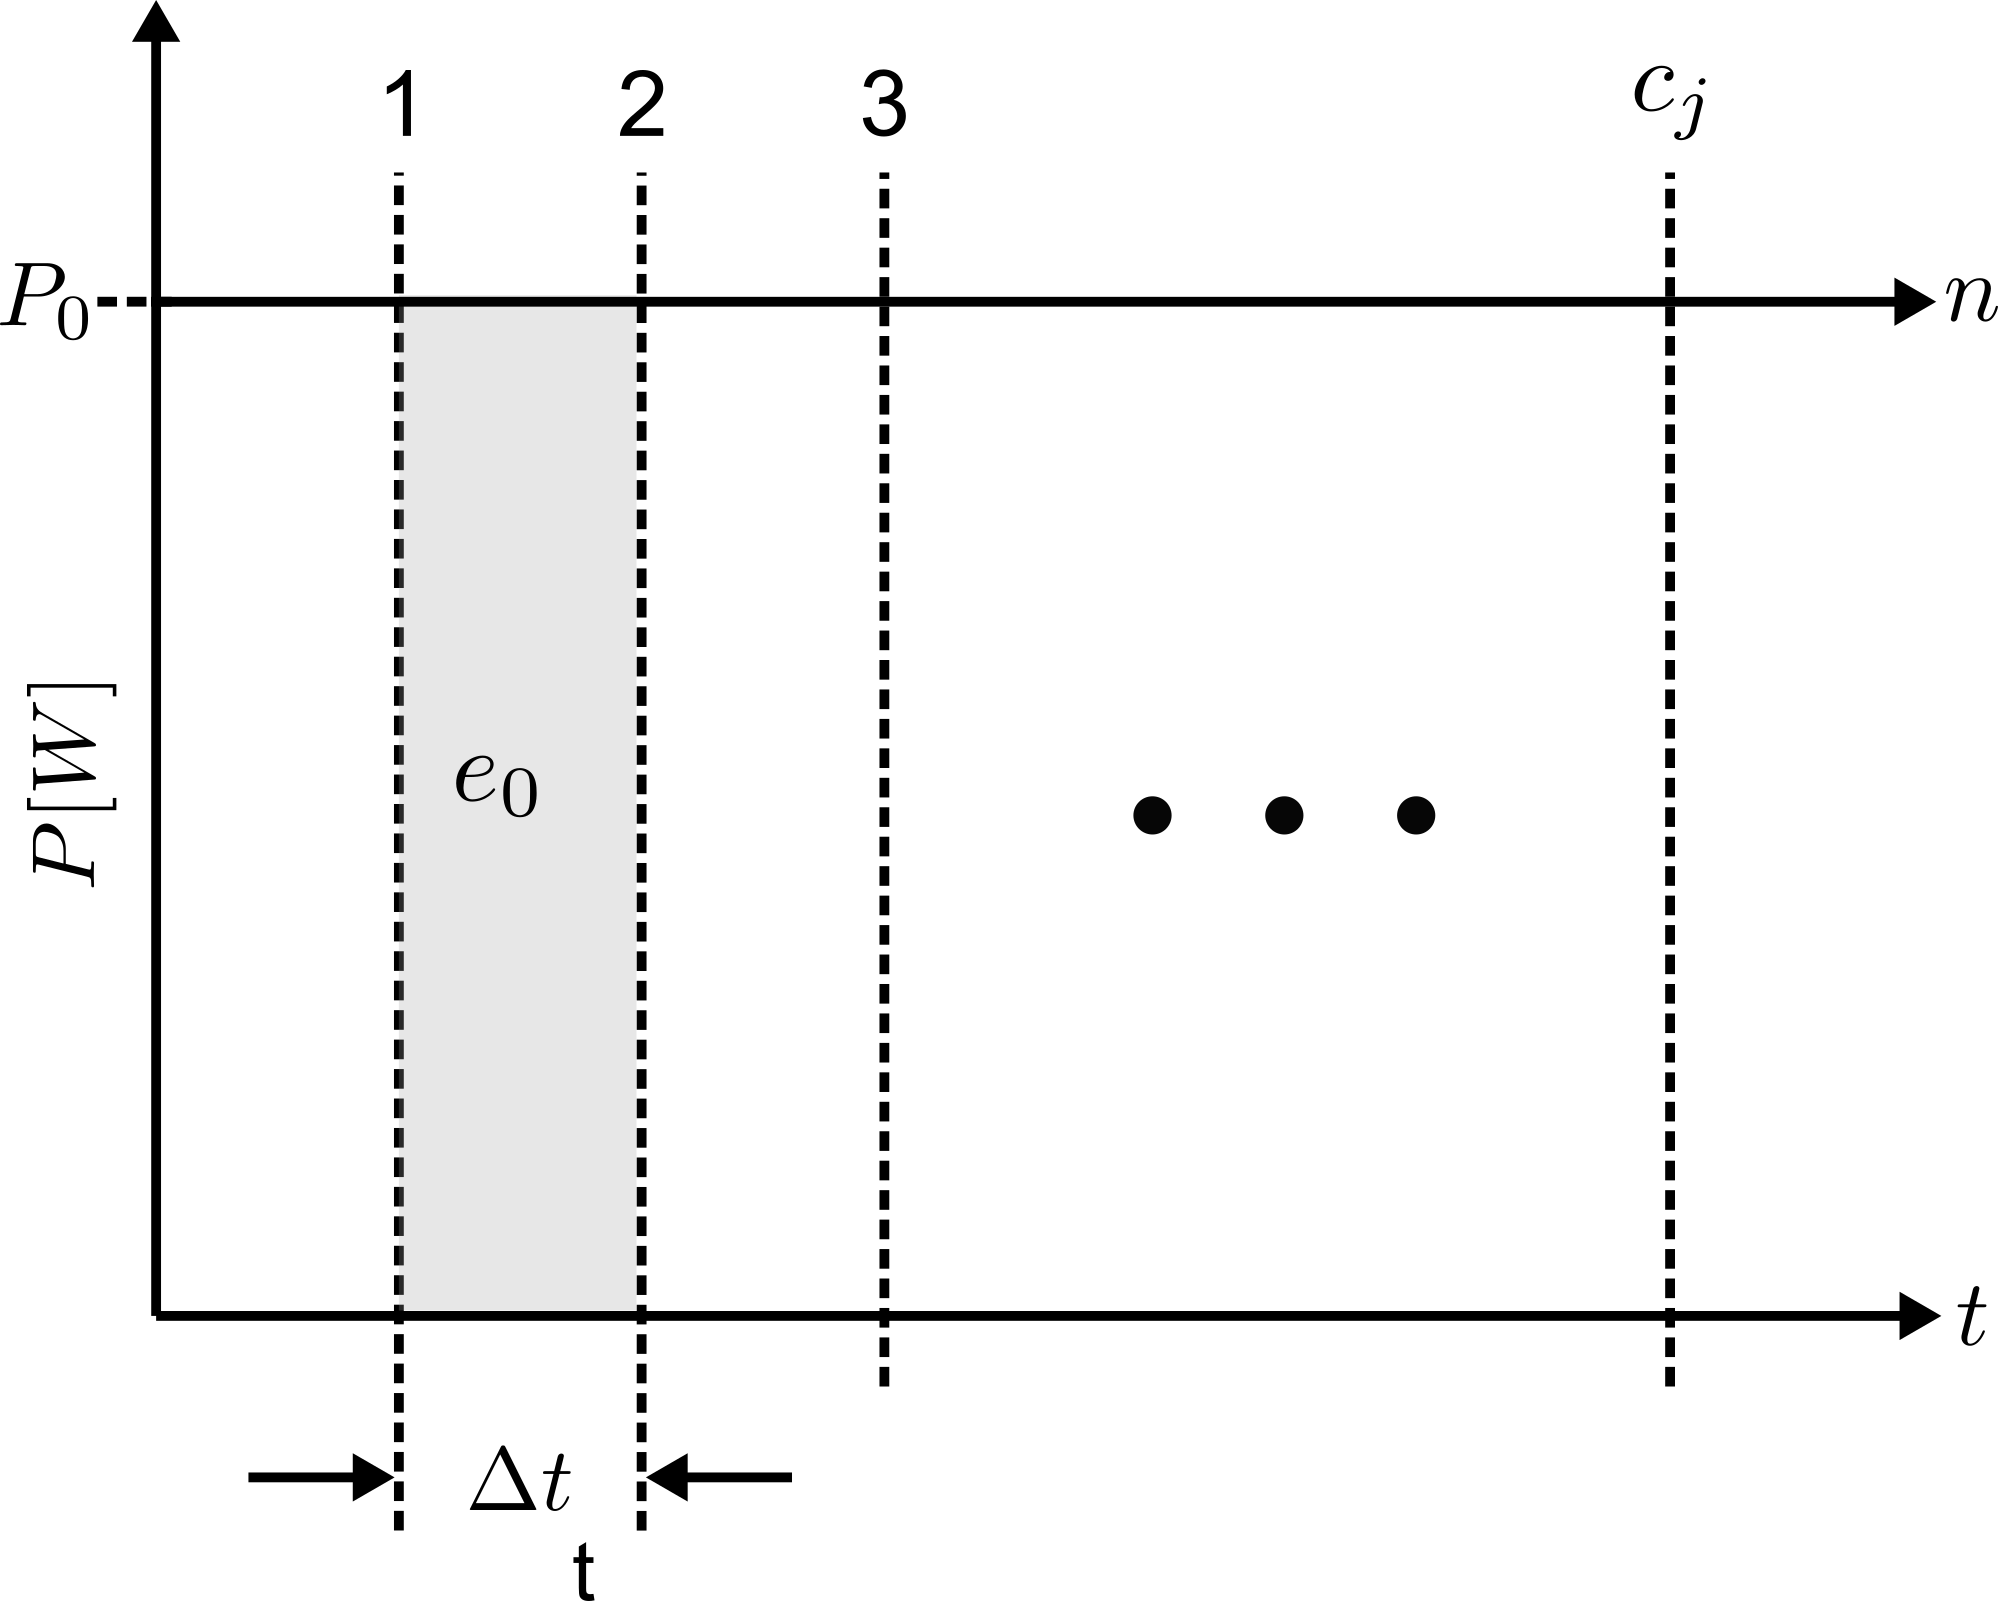
\includegraphics[width=0.45\textwidth]{fig/power_per_episode.png}
	\caption{Power consumption per episode.}
	\label{fig:power_per_episode}
\end{figure}
% ---
\paragraph{Energy requirements.}
Under Asm.~\ref{assumption:power_and_episode_time}, the energy consumption of the $n$-th episode $e_j(n)$ is the constant product
% ---
\begin{equation}\label{eq:energy_per_episode}
	e_j(n) = \underbrace{P_0 \Delta t}_{\text{constant}} = e_0.
\end{equation}
% ---
Consequently, the energy consumed by a robot learning a skill $ s_j $ is directly proportional to the skill complexity $c_j$; i.e.
% ---
\begin{equation}\label{eq:energy_per_skill}
	E_j =\sum_{n=1}^{c_j} e_j(n) = e_0c_j.
\end{equation}
% ---
The energy spent on learning $\mathcal{S}$ under the absence of knowledge transfer is
% ---
\begin{equation}\label{eq:total_energy}
	E_{\mathcal{S}} = \sum_{j=1}^{{N_{\mathcal{S}}}} E_j = e_0 \sum_{j=1}^{{N_{\mathcal{S}}}} c_j%N_{\mathcal{T}} \cdot e_0 \cdot c_j 
\end{equation}
% ---
% ---------------------------------------------------------------------------------------------------
\paragraph{Time requirement.} Similarly, the total learning time $T_{\mathcal{S}}$ for a simple agent is
% ---
\begin{equation}\label{eq:total_time}
	T_{\mathcal{S}} = \Delta t \sum_{j=1}^{{N_{\mathcal{S}}}} c_j.
\end{equation}
% ---

% ===================================================================================================
\subsection{The different learning paradigms}\label{sec:types_of_learning}

% ---------------------------------------------------------------------------------------------------
\paragraph{Isolated Learning (IsL)} A robot performs IsL when it learns each skill in $\mathcal{Z}_k$ one after another from the ground up, disregarding the accumulating knowledge from already learned skills. In such a case the rate of convergence and the initial remaining knowledge for all skills are given by
% ---		
\begin{subequations}\label{eq:fg_isolated}
	\begin{alignat}{2}
		f_{j,k}\left(\cdot \right) &=  -\alpha \\
		g_{j,k}\left(\cdot \right) &= 1,
	\end{alignat}
\end{subequations}
% ---
where $ \alpha>0$ models the rate at which a robot in isolation learns any given skill. Relying on Asm.~\ref{assumption:agent_similarity} we can assign a value to $\alpha$ by using the fundamental complexity $c_0$ as follows
% ---
\begin{equation}\label{eq:isolated_learning_rate}
	\alpha = -\frac{1}{c_0}\text{log}(\epsilon).
\end{equation}
% ---
Since in isolated learning $c^{(IsL)}_{j,k} = c_0$, the trial episodes required by one single robot to learn the skills in the cluster $\mathcal{Z}_k$ is given by
% ---
\begin{equation}
	%	\begin{split}
		%		C^{(IsL)}_{k} &= \sum_{j=1}^{N_{\mathcal{Z}}} c^{(IsL)}_{j,k}= N_{\mathcal{Z}}  \cancelto{c_{0}}{c^{(IsL)}_{j,k}} = N_{\mathcal{Z}} c_0
		%	\end{split}
	C^{(IsL)}_{k} = \sum_{j=1}^{N_{\mathcal{Z}}} c^{(IsL)}_{j,k}= N_{\mathcal{Z}}  c^{(IsL)}_{j,k} = N_{\mathcal{Z}} c_0.
\end{equation}
%-- 
Similarly, the total trial episodes to learn the universe of skills is simply
% ---
\begin{equation}
	C^{(IsL)}_{\mathcal{S}} = N_\mathcal{K} N_{\mathcal{Z}} c_0.
\end{equation}
% ---

\textbf{Multi agent case.} Suppose that a batch of $m$ robots is used to learn the same number of skills in parallel in a given cluster $\mathcal{Z}_k$. Such a strategy only distributes equally the total number of episodes by the number of available robots; i.e.
% ---
\begin{equation}
	^{\lvert \lvert}C^{(IsL)}_k=  \overbrace{\frac{1}{m}C^{(IsL)}_k}^{\text{episodes per robot}}.
\end{equation}
% ---

% ---------------------------------------------------------------------------------------------------
\paragraph{\textbf{Incremental Learning (IL)}}
It corresponds to the continuous aggregation and exchange of knowledge from \emph{intra-cluster} skills. Referring back to Asm.~\ref{assumption:skill_clustering}, the knowledge from skills belonging to a cluster ${\mathcal{Z}_k}$ can be be leveraged by an agent in virtue of their significant similarity. As depicted in Fig.~\ref{fig:intra_skill_learning}, a robot ($r_1$ in this case) learns every skill in $\mathcal{Z}_1$ with a rate $\alpha$ ---the self loops--- but also retains and uses the acquired knowledge to learn subsequent skills. The effect of incremental learning on the knowledge collection rate can be modeled to be directly proportional to the number of learned skills as
% ---
\begin{equation}\label{eq:f_function_incremental}
	f_{j,k}\left(N_{\zeta_k}\right) = -\alpha\left(\eta N_{\zeta_k} + 1 \right), 
\end{equation}
% ---
where $\eta>0$ represents the efficiency of knowledge exchange from $\zeta_k$ to $s_{j,k}$. Different potential models might be used to model the depletion of the initial remaining knowledge represented by $g_{j,k}\left(N_{\zeta_k}\right)$, e.g. a linear decay rate, our expectation is that, under the assumption that a learning strategy involving the ordering of skills according to similarity and their balanced distribution in the different clusters, $g_{j,k}\left(N_{\zeta_k}\right)$ might naturally resemble an exponential decay that is strongly dependent on $N_{\zeta_k}$. Such considerations motivate our choice of the following function
% ---
\begin{equation}\label{eq:g_function_incremental}
	g_{j,k}\left(N_{\zeta_k}\right) = e^{-\delta N_{\zeta_k}},
\end{equation}
%---
again with a factor $\delta>0$ controlling the rate at which the exponential converges. Similar to $\alpha$, using Asm.~\ref{assumption:cluster_size} $\delta$ can be defined as 
% ---
\begin{equation}\label{eq:delta}
	\delta = -\frac{1}{N_\mathcal{Z}}\text{log}(\epsilon).
\end{equation}
% ---
Essentially, such choice of $\delta$ implies that the remaining knowledge in a cluster after seeing all its skills is negligible. Via the exchange factors $(\eta,\delta)$, in incremental learning the knowledge about every new skill gets gradually increased by leveraging previous knowledge, resulting in
% ---
\begin{equation*}\label{eq:remaining_knowledge__IL}
	\bar{\sigma}^{(IL)}_{i,j}(n) = e^{-\alpha  \left(\eta N_{\zeta_k}+1\right) n} e^{-\delta N_{\zeta_k}}.
\end{equation*}
% ---
As the complexity $c_{j,k}$ of a skill can also be interpreted as the number of trial episodes required for the remaining knowledge to go below a threshold $\epsilon$; i.e.
% ---
\begin{equation*}
	\bar{\sigma}^{(IL)}_{i,j}(n) \Big \rvert_{n \ge c^{(IL)}_{j,k}} \leq \epsilon.
\end{equation*}
% ---
Then, under this scheme the complexity $c^{(IL)}_{j,k}$ to learn a new is skill in the cluster results in
% ---
\begin{equation}\label{eq:complexity_IL}
	c^{(IL)}_{j,k} = -\frac{\text{log}(\epsilon) - \text{log}\left(\bar{\sigma}^{(IL)}_{j,k}(0)\right)}{\alpha (\eta N_{\zeta_k}+ 1)} = -\frac{\text{log}(\epsilon) + \delta N_{\zeta_k}}{\alpha (\eta N_{\zeta_k}+ 1)}  .
\end{equation}
% ---
The total number of trial episodes $ C_k $ that an agent following an incremental learning strategy needs to learn the $N_{\mathcal{Z}_k}$ skills in a cluster $ \mathcal{Z}_k $ is given by
% ---
\begin{align}\label{eq:total_episodes_incremental}
	\begin{split}
		C^{(IL)}_k &= \sum^{N_{\mathcal{Z}}}_{j=1} c^{(IL)}_{j,k}.
	\end{split}
\end{align}
% ---

\textbf{Multi-agent case.} If $m$ robots are used in parallel to divide the load of learning the tasks then
% ---
\begin{align}
	\begin{split}
		{}^{\lvert \rvert}C^{(IL)}_k &= \sum^{\frac{N_{\mathcal{Z}}}{m}}_{j=1} c^{(IL)}_{j,k}.
	\end{split}
\end{align}
% --
In essence, using $m$ robots without exchanging knowledge only subdivides the learning in every cluster into $m$ smaller problems \emph{without adding any additional benefit to the rate at which knowledge is acquired}. 

% ---------------------------------------------------------------------------------------------------
\paragraph{\textbf{Transfer + Incremental Learning (TIL)}}
Transfer learning (TL) alone refers to the one-time \emph{inter-cluster} exchange of knowledge. Considering $\mathcal{K} = \{ \mathcal{Z}_k \}^{N_\mathcal{K}}_{k=1}$ to be the set of all available skill clusters, TL represents the exchange of knowledge from the skills learned in different \emph{origin} clusters $\mathcal{O} = \{ \mathcal{Z}_1,\mathcal{Z}_2,\ldots,\mathcal{Z}_{k-1} \}$ to the skills that will be learned in a \emph{destination} cluster $\mathcal{Z}_k$ (see Fig.~\ref{fig:cluster_to_cluster_knowledge_transfer_parallel}). Concretely, the effect that TL has on the skills of the destination cluster is the reduction of the initial remaining knowledge and the increase of the initial learning rate for all the skills in the $k$-th cluster via the parameter $\beta_k$; i.e.
% ---
\begin{equation}\label{eq:f_function_transfer}
	f_{j,k}\left(N_{\zeta_k}\right) = -\alpha \left( \frac{\eta N_{\zeta_k} + 1}{1 - \beta_k} \right),
\end{equation}
% ---
and
% ---
\begin{equation}\label{eq:g_function_transfer}
	g_{j,k}\left(N_{\zeta_k}\right) = (1-\beta_k) e^{-\delta N_{\zeta_k}}.
\end{equation}
%---
In essence, $\beta_k$ is the head start granted by knowledge transfer from other clusters to the skills in $\mathcal{Z}_k$. We argue that  $0<\beta_{k} < 1$ since it represents the \emph{aggregated} knowledge exchange factor from the different origin clusters $\mathcal{Z}_{c}$ to the target cluster $\mathcal{Z}_{k}$. Let $0<\beta_{c} < 1$ be the transfer contribution factor of a single origin cluster $\mathcal{Z}_c$. Additionally, consider that
% ---
\begin{equation}
	\sum\limits_{c=1}^{N_\mathcal{K}}\beta_{c} \leq 1,
\end{equation}
% --
as $1$ represents all the knowledge in $\mathcal{S}$. Asm.~\ref{assumption:cluster_transferability} implies that $\beta_c$ is equal for all the clusters. In this work we select $\beta_c = 1/N_\mathcal{K}$ for simplicity. The aggregated transfer factor $\beta_k$ is the sum of the individual factors from the already-visited clusters; i.e.
% ---
\begin{equation}\label{eq:beta_k_transfer}
	\beta_{k}= \left(k-1\right)\beta_c = \left(k-1\right)\frac{1}{N_\mathcal{K}}.
\end{equation}
% ---

Consequently, the remaining knowledge when transfer and incremental learning are used in conjunction is
% ---
\begin{equation}\label{eq:remaining_knowledge__ITL}
	\bar{\sigma}^{(TIL)}_{j,k}(n) = \left(1- \beta_k\right) e^{-\alpha  \left(\frac{ \eta N_{\zeta_k}+1}{1 - \beta_k}\right) n} e^{-\delta N_{\zeta_k}}.
\end{equation}
% ---
Similar to incremental learning, the complexity to learn a skill in transfer learning is
\begin{equation}\label{eq:skill_complexity_TL}
	c^{(TIL)}_{j,k} = -\frac{1 - \beta_{k}}{\alpha (\eta N_{\zeta_k}+ 1)}\left[\text{log}(\epsilon) + \delta N_{\zeta_k} - \text{log}(1 - \beta_{k})\right]
\end{equation}
% ---
and the total number of episodes  $ C_k $ that an agent requires to learn the $N_{\mathcal{Z}_k}$ skills is merely their sum
% ---
\begin{align}\label{eq:total_episodes_transfer}
	\begin{split}
		C^{(TIL)}_k &= \sum^{N_{\mathcal{Z}}}_{j=1} c^{(TIL)}_{j,k}.
	\end{split}
\end{align}
% --- 

\textbf{Multi-agent case.} If $m$ robots are used in parallel to divide the load of learning the tasks then, the transfer of knowledge from cluster to cluster is also divided by the number of robots, this implies that \eqref{eq:beta_k_transfer} changes to
% ---
\begin{equation}\label{eq:beta_k_transfer_parallel}
	{}^{\lvert \rvert}\beta_{k}= \frac{1}{m}\beta_{k}.
\end{equation}
% ---
Correspondingly, when using transfer learning in parallel $\beta_k$ is replaced by ${}^{\lvert \rvert}\beta_{k}$ in \eqref{eq:skill_complexity_TL}. Then, similar to IL, the total number of episodes to learn the skills in a cluster is
% ---
\begin{align}
	\begin{split}
		{}^{\lvert \rvert}C^{(TIL)}_k &= \sum^{\frac{N_{\mathcal{Z}}}{m}}_{j=1} c^{(TIL)}_{j,k}.
	\end{split}
\end{align}
% ---
This case is depicted on Fig.~\ref{fig:cluster_to_cluster_knowledge_transfer_parallel}, where two robots $ r_1$ and $r_2$ learn skills in four different clusters. The shaded areas are the subclusters of skills learned by each robot. Since they do not share knowledge between them, each robot has access only to the knowledge it has collected and cannot benefit from one another. 

% ---------------------------------------------------------------------------------------------------
%\subsection*{\textbf{Collective learning (CL)}}
%As mentioned in Sec.~\ref{sec:intro}, EAI agents will be a core element of industrial, healthcare, and domestic ecosystems with advanced communication and remote processing capabilities. Given the anticipated legions of EAI agents executing and learning several different skills at any given time in those environments, it is immediately evident that the previous learning paradigms are not meant to exploit these large number of agents together with the advanced communication and processing infrastructure to take full advantage of the potential for concurrent knowledge exchange among the agents. Therefore, the use of isolated, incremental, and transfer learning by these many agents 
%would directly aggravate computational demand (see challenge C1). As discussed in \cite{Kaelbling2020foundationefficientrobot} an leaning algorithm that would allow an agent to learn new tasks on-the-fly would need to be sample-efficient, generalizable, compositional, and (truly) incremental. Collective learning is the natural paradigm that meets this requirements exploiting the full communication potential of the networked EAI agents to leverage the real-time synergistic exchange and aggregation of collected knowledge to make the learning of tasks energy- and time-efficient.
%
%To formalize this idea, let $ \left\lbrace \rho_i \right\rbrace_{i=1}^{m} $ be a set of robotic agents that defines a community of robots. In collective learning, the different robotic agents $ \rho_i $ develop and accumulate dynamically a common mind (body of knowledge) via networked interactions where individual experience, knowledge and skills are disseminated to all the other elements in the collective. Information flows vertically as previous knowledge is passed on, as well as horizontally by sharing concurrent experience between agents. Via these mechanisms, knowledge can be replicated, complimented and further developed. We take from \cite{Garavan2012CollectiveLearning} two notions central in collective learning that are applicable to the embodied AI agents:
%% ---
%\begin{enumerate}
%	\item Capability to restructure and meet changing conditions
%	\item Aggregation of skills, knowledge, and behaviors
%\end{enumerate}
%% ---
%Collective learning contrasts with the previously discussed incremental learning in that a single agent $ r_i $ can aggregate only so much knowledge via trial and error and is limited by a sequential learning structure. Learning collectively, on the other hand, enforces parallelization of knowledge acquisition via the concurrent learning and sharing of all agents as they acquire new skills, knowledge. Moreover, collective learning involves not only the information acquisition, but also how this information is brought to use to form and develop knowledge. 
%
%CL is not only a promising research direction but, in our opinion, has the potential to be a unifying solution to the grand challenges posed by embodied AI. Furthermore, by incorporating new mechanical designs as elements of the learning pipeline it is possible to iteratively evaluate the energy efficiency of proposed solutions and select the best ones as reference designs for future manufacturing processes with underlying learning, therefore, promoting a cyclical optimization towards a semi-optimal general design.
%
%Unlike isolated and transfer learning, in this paradigm a batch of robots $\left \lbrace r_i \right \rbrace^m_{1}$ not only learn different skills concurrently but also exchange the acquired knowledge between each other and are actually able to leverage it. To enable CL, it is assumed that
%\begin{itemize}
%	\item an inter-agent communication protocol/infrastructure is in place that
%	\item enables agents to concurrently exchange and integrate the self-acquired and received knowledge to
%	\item incrementally speed up the learning of all the agents as a whole.
%\end{itemize}
%% ---
%As a result, the intra- and inter-cluster knowledge transfer is possible. Naturally, the CL paradigm involves a complex scheduling problem to determine the optimal skill distribution and inter-agent knowledge sharing strategy. Since we have not tackled this problem yet, we ground the subsequent discussion on Assumptions~\ref{assumption:average_behavior}, \ref{assumption:agent_similarity},~\ref{assumption:cluster_size}, and~\ref{assumption:cluster_transferability} that suggest an average behavior given a suitable scheduling.
%
%Fig.~\ref{fig:cl_example_figure} illustrates the CL concept, where the self loop represents the dynamics of a single robot learning (at a rate $\alpha$). The exchange of knowledge across agents is represented via the cross-couplings weighted by a parameter $\gamma$ that models how efficient is the bidirectional pairwise knowledge exchange. Similar to transfer learning, if two robots exchange knowledge about skills with low similarity (i.e. skills in different clusters), then $\gamma$ is scaled by the inter-cluster transferability parameter $\beta$. In CL \eqref{eq:simple_knowledge_dynamics} is extended to 
%% ---
%\begin{subequations}\label{eq:collective_knowledge_dynamics}
%	\begin{empheq}[left=\empheqlbrace]{align}
%		\dot{\bar{\bm{\sigma}}}^{(CL)}_{j,k}\left(n\right) &= \left[  f_{j,k}\left(N_{\zeta_k},r\right) \bm{I} + \gamma \bm{A} \odot \bm{B}  \right] \bar{\bm{\sigma}}^{(CL)}_{j,k}\left(n\right)\\
%		\bar{\bm{\sigma}}^{(CL)}_{j,k}(0) &= g_{j,k}\left( N_{\zeta_k}, r\right) \bm{I},
%	\end{empheq}
%\end{subequations}
%% ---
%where $r=m$ is the number of robots that exchange knowledge among them. This implies that now $\bar{\bm{\sigma}}^{}_{j,k} \in \mathbb{R}^r$ is a vector that represents the dynamics of the remaining knowledge of all the $m$ skills being concurrently learned. $\bm{A} \in \mathbb{R}^{r \times r}$ is a zero-diagonal symmetric adjacency matrix whose entry $(\bm{A})_{i,j} = 1$ if robot $i$ exchanges knowledge with robot $j$ and $(\bm{A})_{i,j} = 0$ if it does not. The term $\gamma \in \mathbb{R}_+ $ weighs the knowledge exchange strength among robots. Furthermore, since there may be robots learning skills in different clusters at the same time, the matrix $\bm{B}$, whose entries are $\left(\bm{B}\right)_{i,j} \in \left \lbrace 1, \beta_{k} \right \rbrace$, with
%% ---
%\begin{equation}
%	%\beta_{k} = 1/N_\mathcal{K}, 
%	\beta_{k} = r\frac{ N_{\zeta_k}}{N_\mathcal{S}}, 
%\end{equation}
%% ---
%scales down the knowledge contributions between robots from different clusters. Finally, the operator $\odot$ represents the Hadamard product of matrices. The functions $ f(\cdot)$ and $g(\cdot)$ are now also dependent on the number of robots that exchange knowledge, which directly impacts the number of skills that enter $\zeta_k$ after a learning cycle; i.e.
%% ---
%\begin{equation}\label{eq:f_function_collective}
%	f_{j,k}\left(N_{\zeta_k},r\right) = -\alpha \left( \frac{\eta r N_{\zeta_k} + 1}{1 - \beta_k} \right),
%\end{equation}
%% ---
%and
%% ---
%\begin{equation}\label{eq:g_function_collective}
%	g_{j,k}\left(N_{\zeta_k},r\right) = (1-\beta_k) e^{-\delta r N_{\zeta_k}}.
%\end{equation}
%%---
%Some considerations need to be taken when selecting the value of $\gamma$ given that the dynamics matrix of the collective system
%% ---
%\begin{equation}
%	\bar{\bm{A}}\left(N_{\zeta_k}\right) = f\left(N_{\zeta_k},r\right) \bm{I} + \gamma \bm{A} \odot \bm{B} 
%\end{equation} 
%% ---
%exhibits a dependency on the number of seen skills $N_{\zeta_k}$, which is directly influenced by the number of robots $r$ in the collective. Yet, it can be proven that there is a coupling strength $\gamma$ for a given connectivity $\bm{A}$ that ensures that the remaining knowledge for all skills converges asymptotically to zero.


% ===================================================================================================
%                                                 |                                                 |
%                                                 |                                                 |
% -------------------------------------------- SECTION ---------------------------------------------|
%                                                 |                                                 |
%                                                 |                                                 |
% ===================================================================================================
\newpage
\section{Results}\label{sec:use_case_results}
Fig.~\ref{fig:collective_learning} shows the results of applying isolated learning, incremental learning, transfer and incremental learning, and collective learning to the learning scenario defined by the tuple
% ---
\begin{equation*}
	\phi_{SF} = \left(N_\mathcal{S}= 512, N_\mathcal{K}=4, m=32, \left[\alpha =  0.0461, \delta =  0.0360, \eta= 0.1\right]\right).
\end{equation*}
% ---
In this scenario all $m$ agents are always concurrently learning skills from the same cluster $Z_i$.
% ---
\begin{figure}[!h]
	\centering
	\hspace*{\fill}
	\subfloat[]{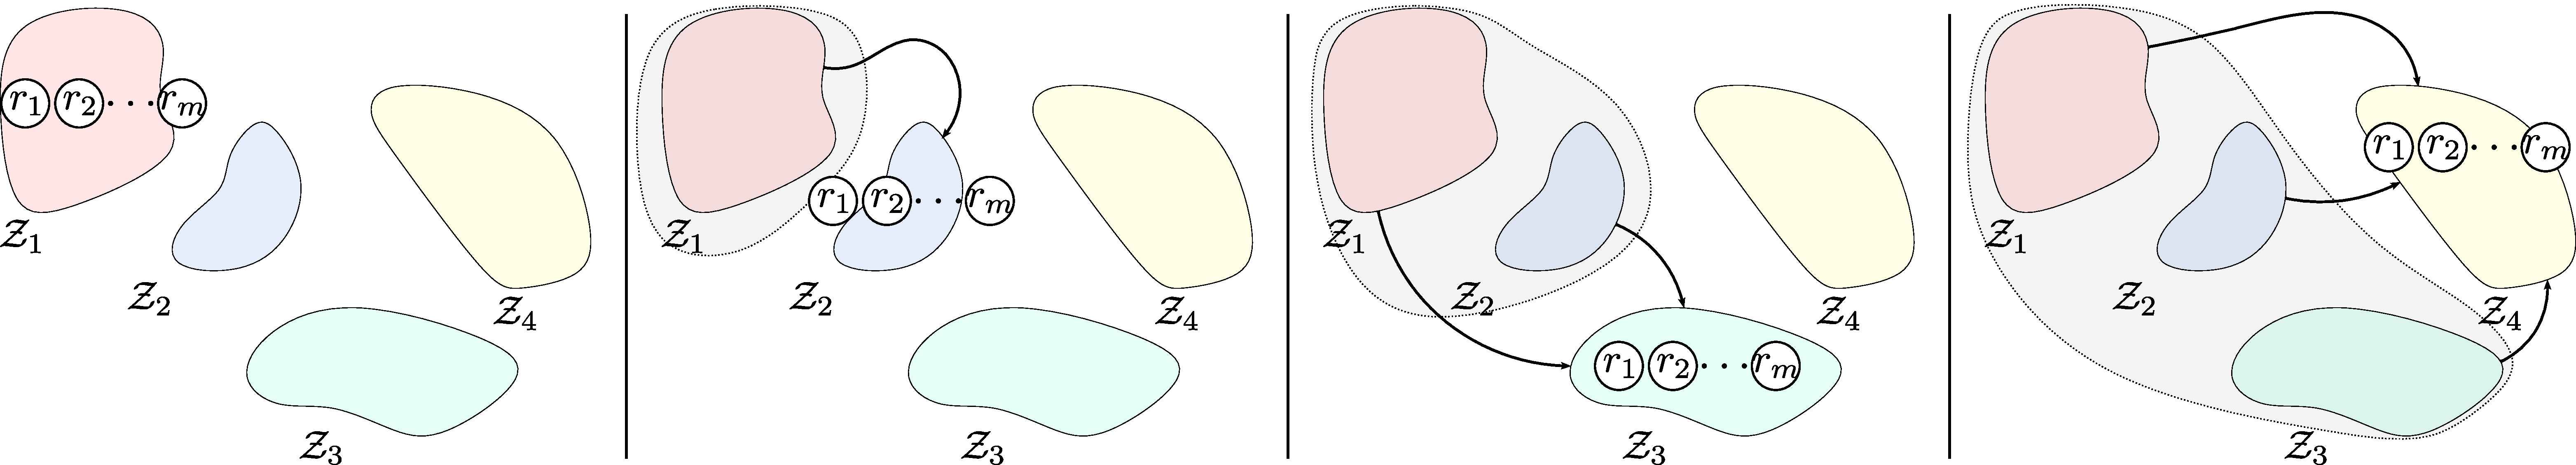
\includegraphics[width= 0.7\textwidth]{fig/cluster_learning_sequence.png} \label{fig:cluster_learning_sequence}}
	\hspace*{\fill}
	\\	
	\hspace*{\fill}
	\subfloat[]{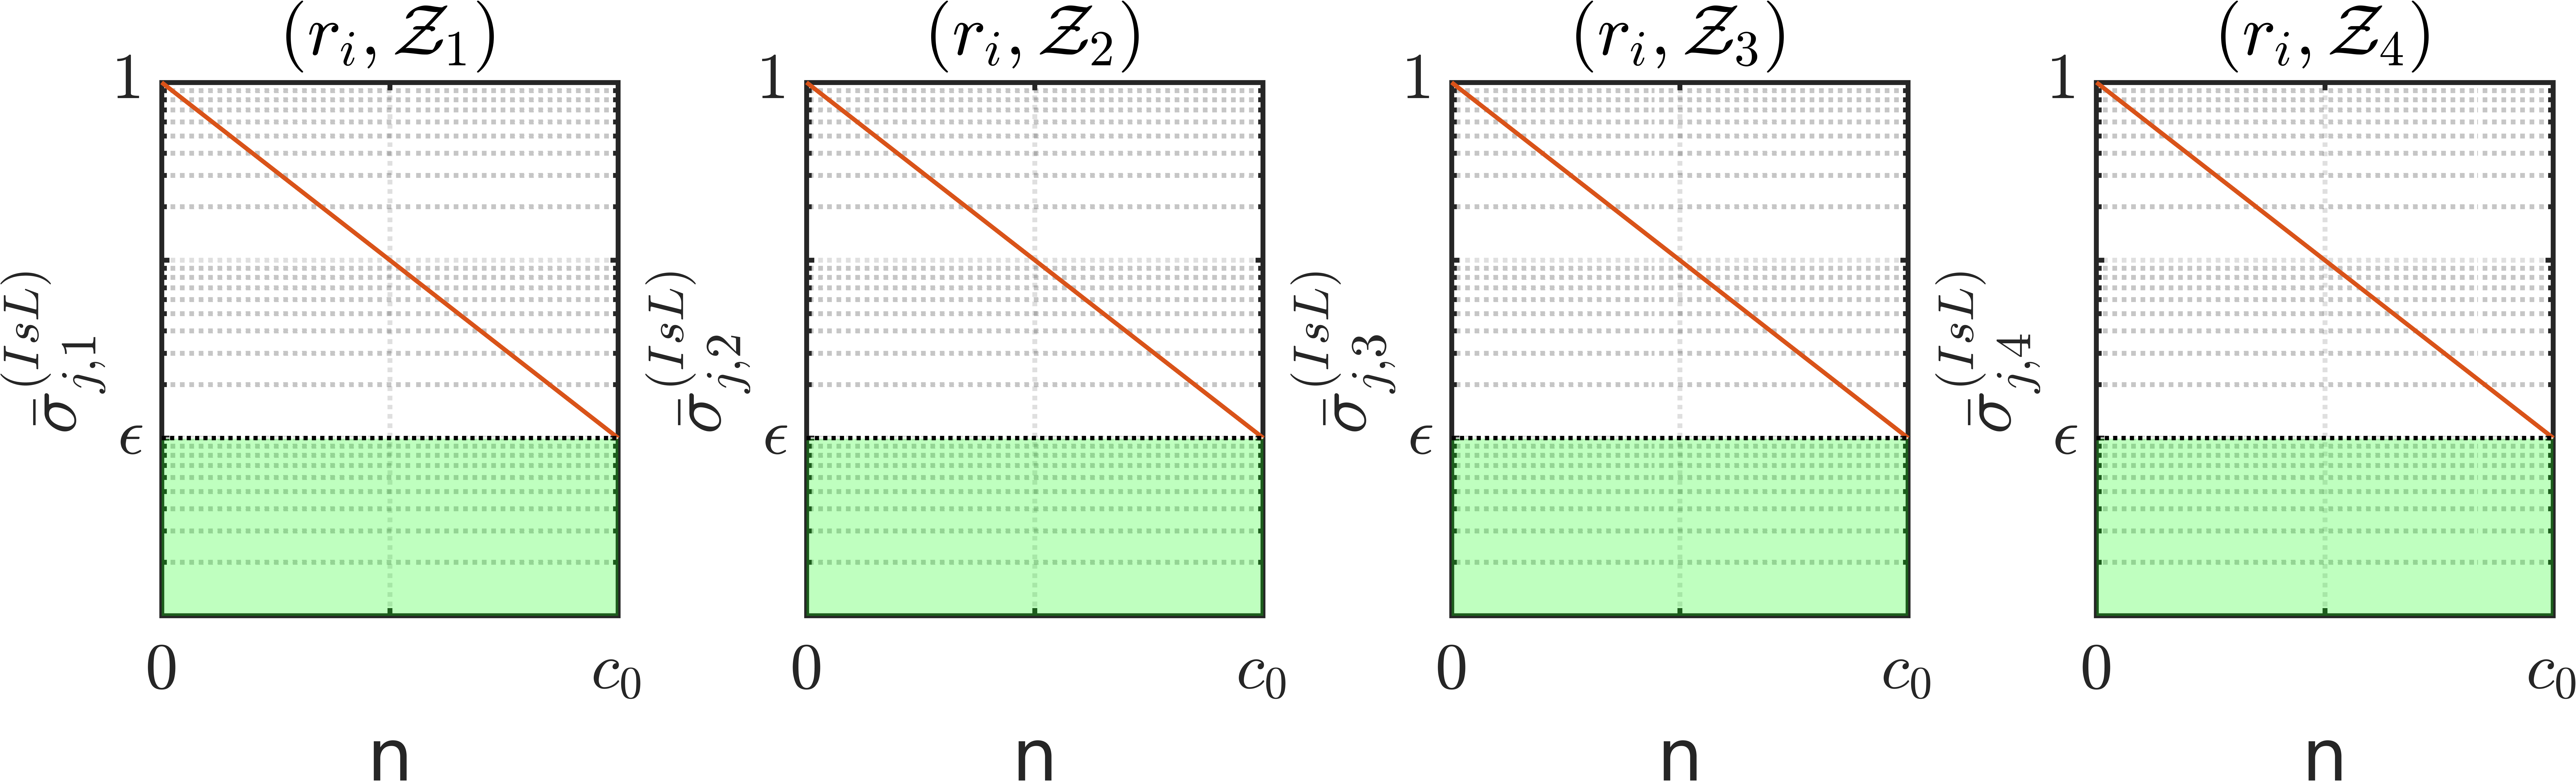
\includegraphics[width= 0.7\textwidth]{fig/dynamics_isolated_learning.png} \label{fig:dynamics_isolated_learning}}  
	\hspace*{\fill}
	\\	
	\hspace*{\fill}
	\subfloat[]{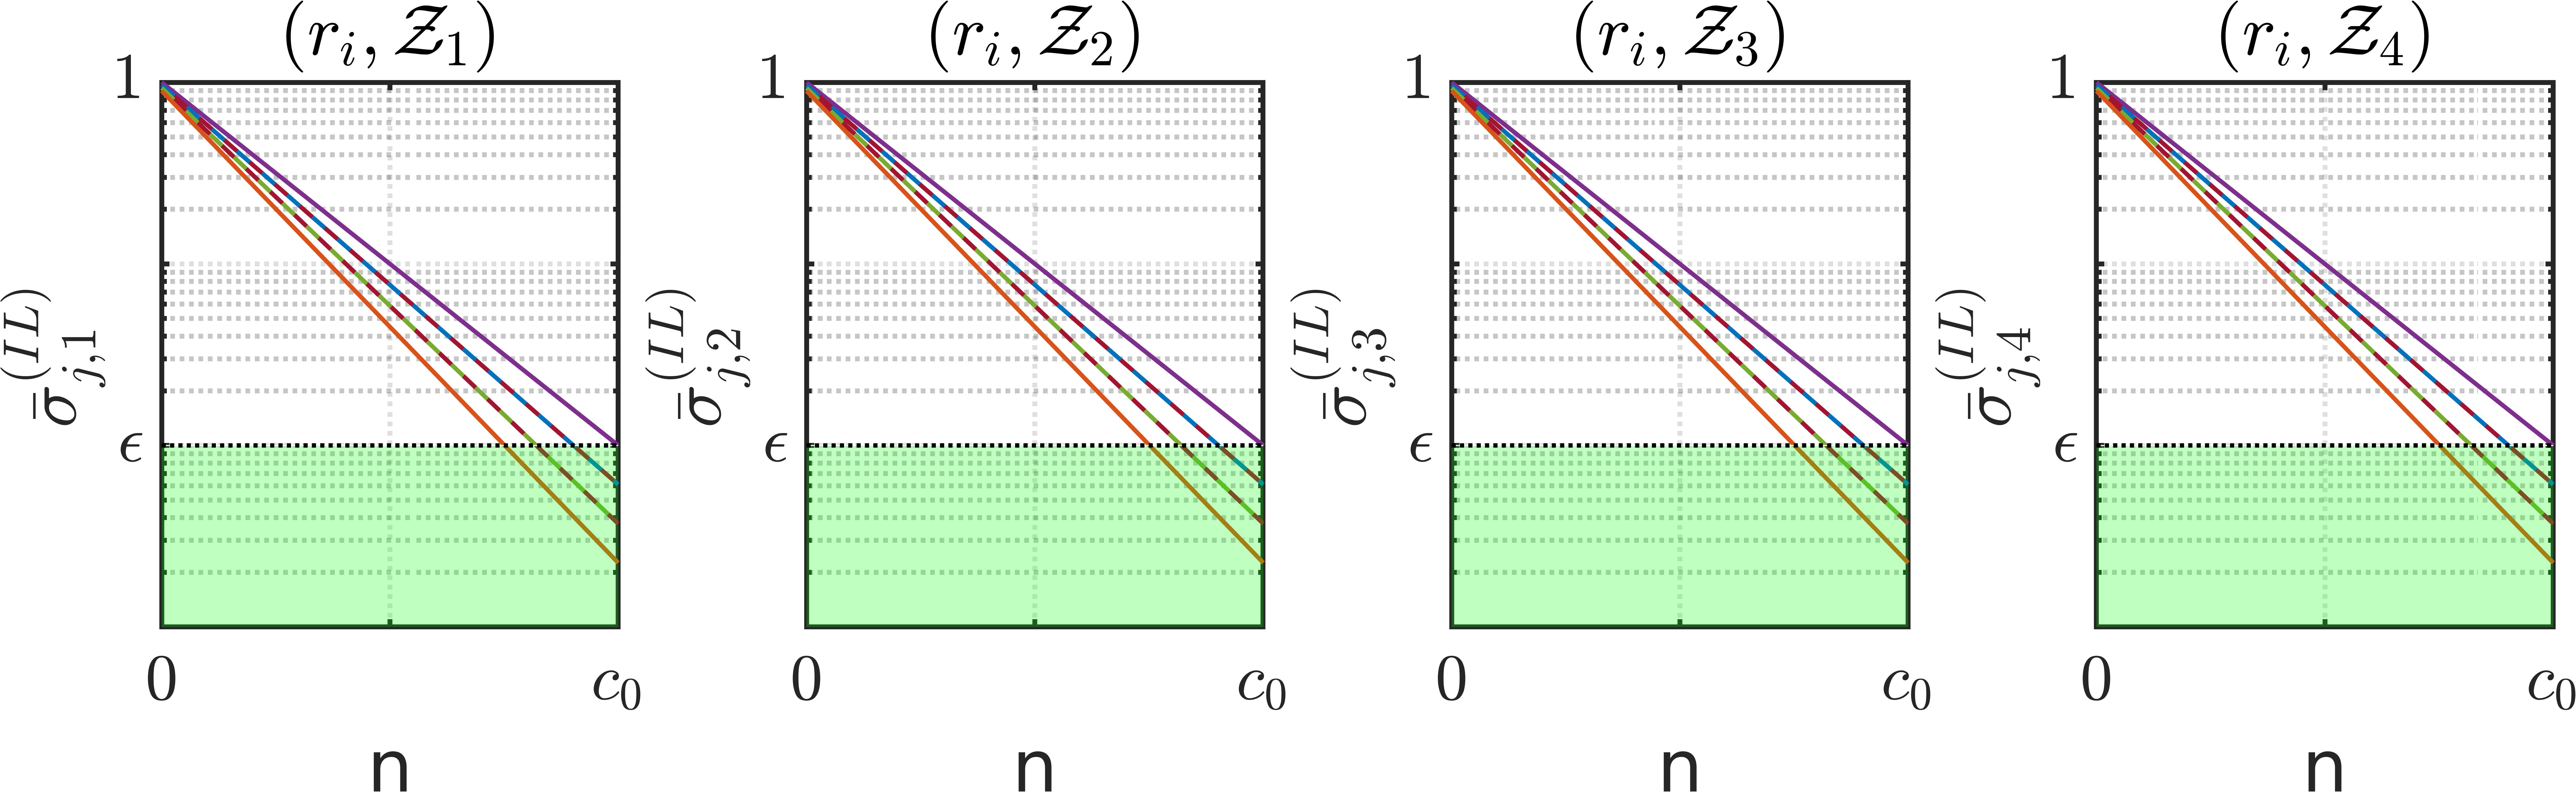
\includegraphics[width= 0.7\textwidth]{fig/dynamics_incremental_learning.png} \label{fig:dynamics_incremental_learning}}  
	\hspace*{\fill}	
	\\
	\hspace*{\fill}
	\subfloat[]{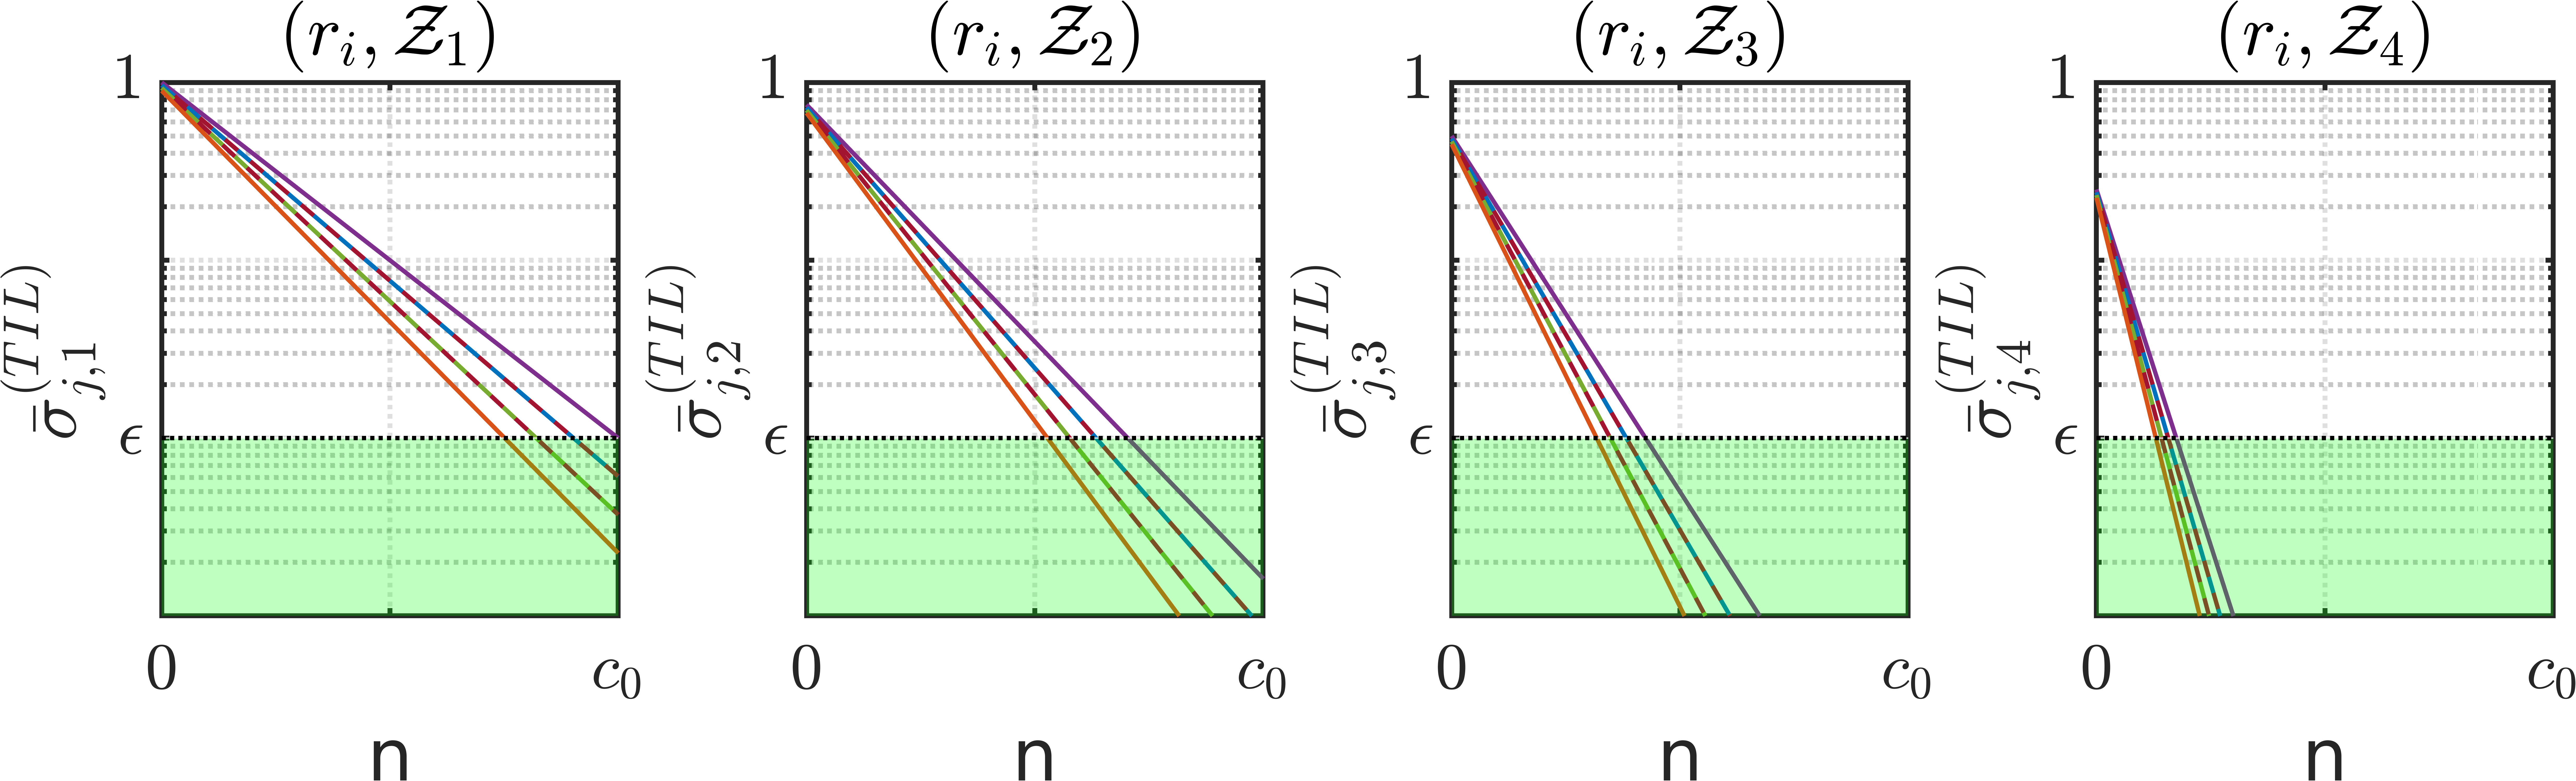
\includegraphics[width= 0.7\textwidth]{fig/dynamics_incremental_transfer_learning.png} \label{fig:dynamics_incremental_transfer_learning}}  
	\hspace*{\fill}
	\\
	\hspace*{\fill}
	\subfloat[]{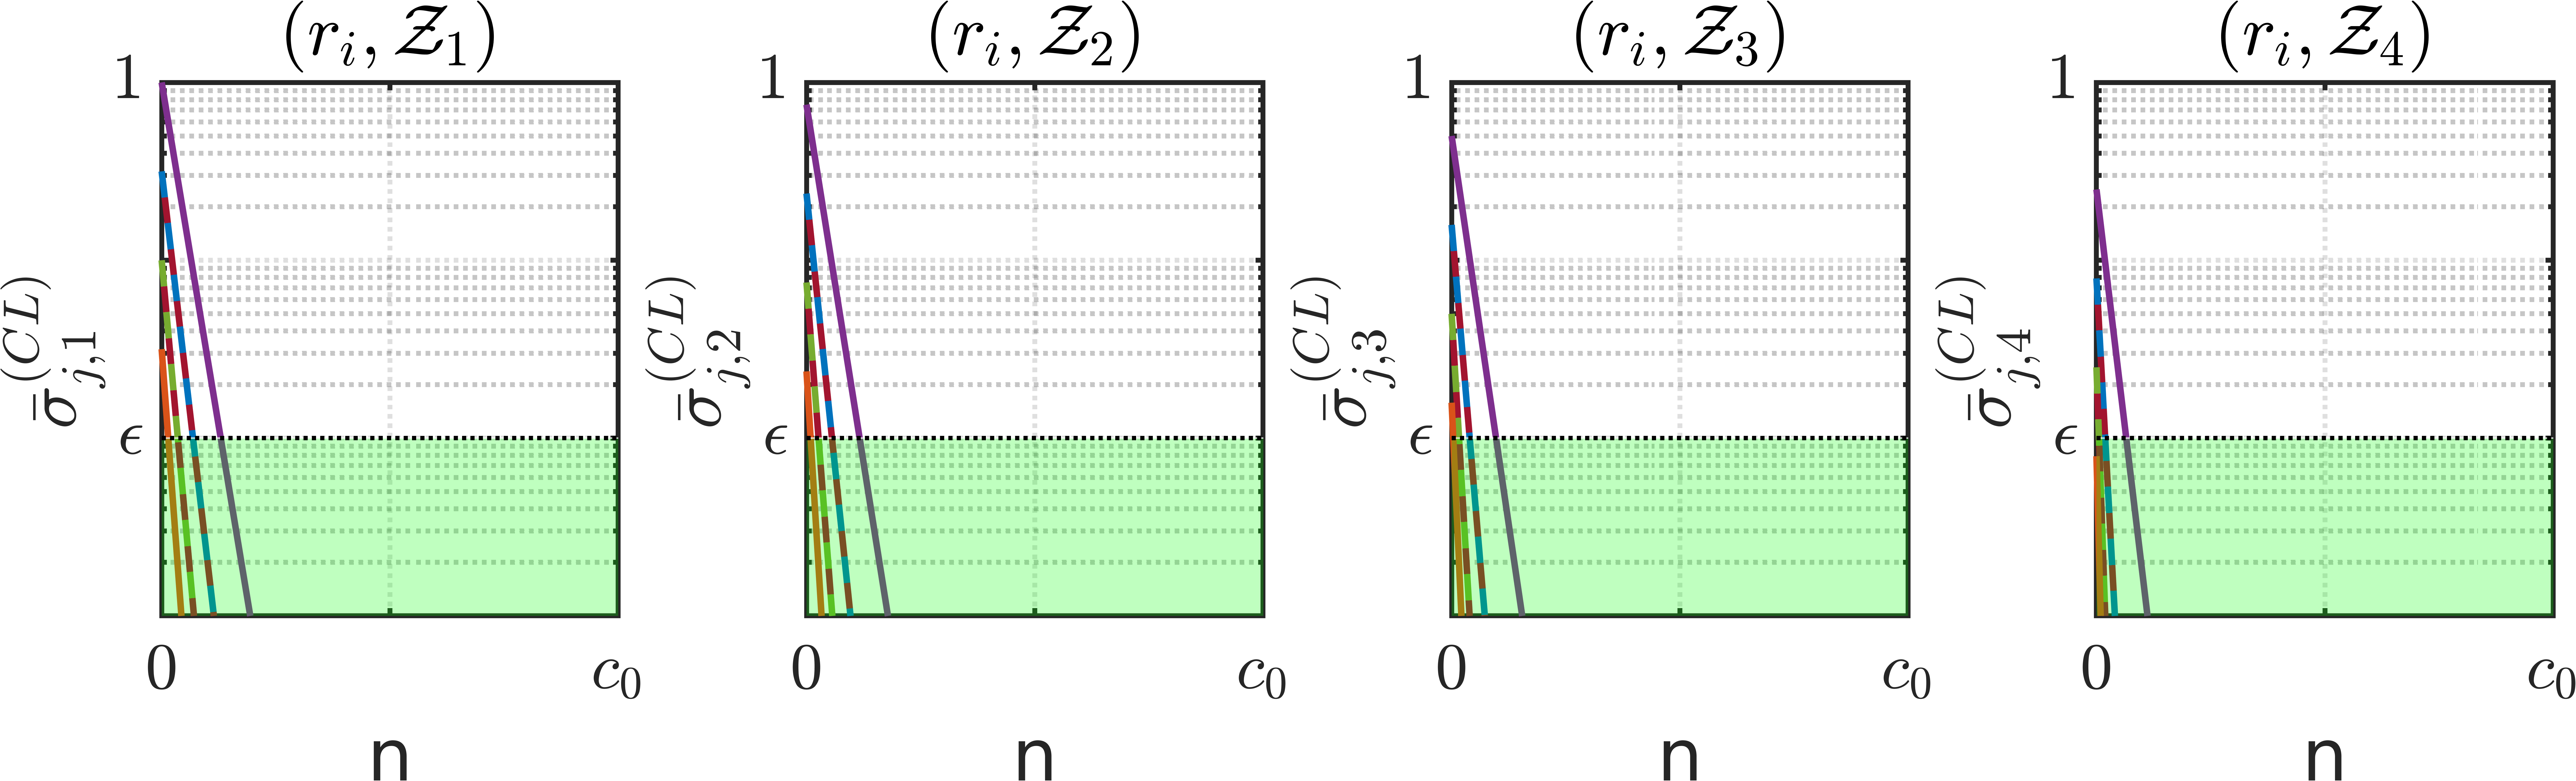
\includegraphics[width= 0.7\textwidth]{fig/dynamics_collective_learning.png} \label{fig:dynamics_collective_learning}}
	\hspace*{\fill}
	\caption[] {\label{fig:collective_learning} Scenario 1: \subref{fig:cluster_learning_sequence} the skills of each cluster are learned by the $ m$ robots in succession, \subref{fig:dynamics_isolated_learning} isolated learning, \subref{fig:dynamics_incremental_learning} incremental learning,  \subref{fig:dynamics_incremental_transfer_learning} incremental + transfer learning, \subref{fig:dynamics_collective_learning} collective learning.}
\end{figure}
% ---


% ===================================================================================================
%                                                 |                                                 |
%                                                 |                                                 |
% -------------------------------------------- SECTION ---------------------------------------------|
%                                                 |                                                 |
%                                                 |                                                 |
% ===================================================================================================
\newpage
\section{Supporting statistics}
% ===================================================================================================
\subsection{Industrial and cobot statistics}\label{sec:robot_statistics}
According to the International Federation of Robotics (IFR) the unit sales of collaborative robots in relation to conventional industrial robots has been constantly increasing in the past years \cite{statista_ir_cobot_share}. Recent data, see Fig.~\ref{fig:industrial_cobot_share}, shows that cobots now make almost 15 \% of the sales.
%---
\begin{figure}[!h]
	\centering
	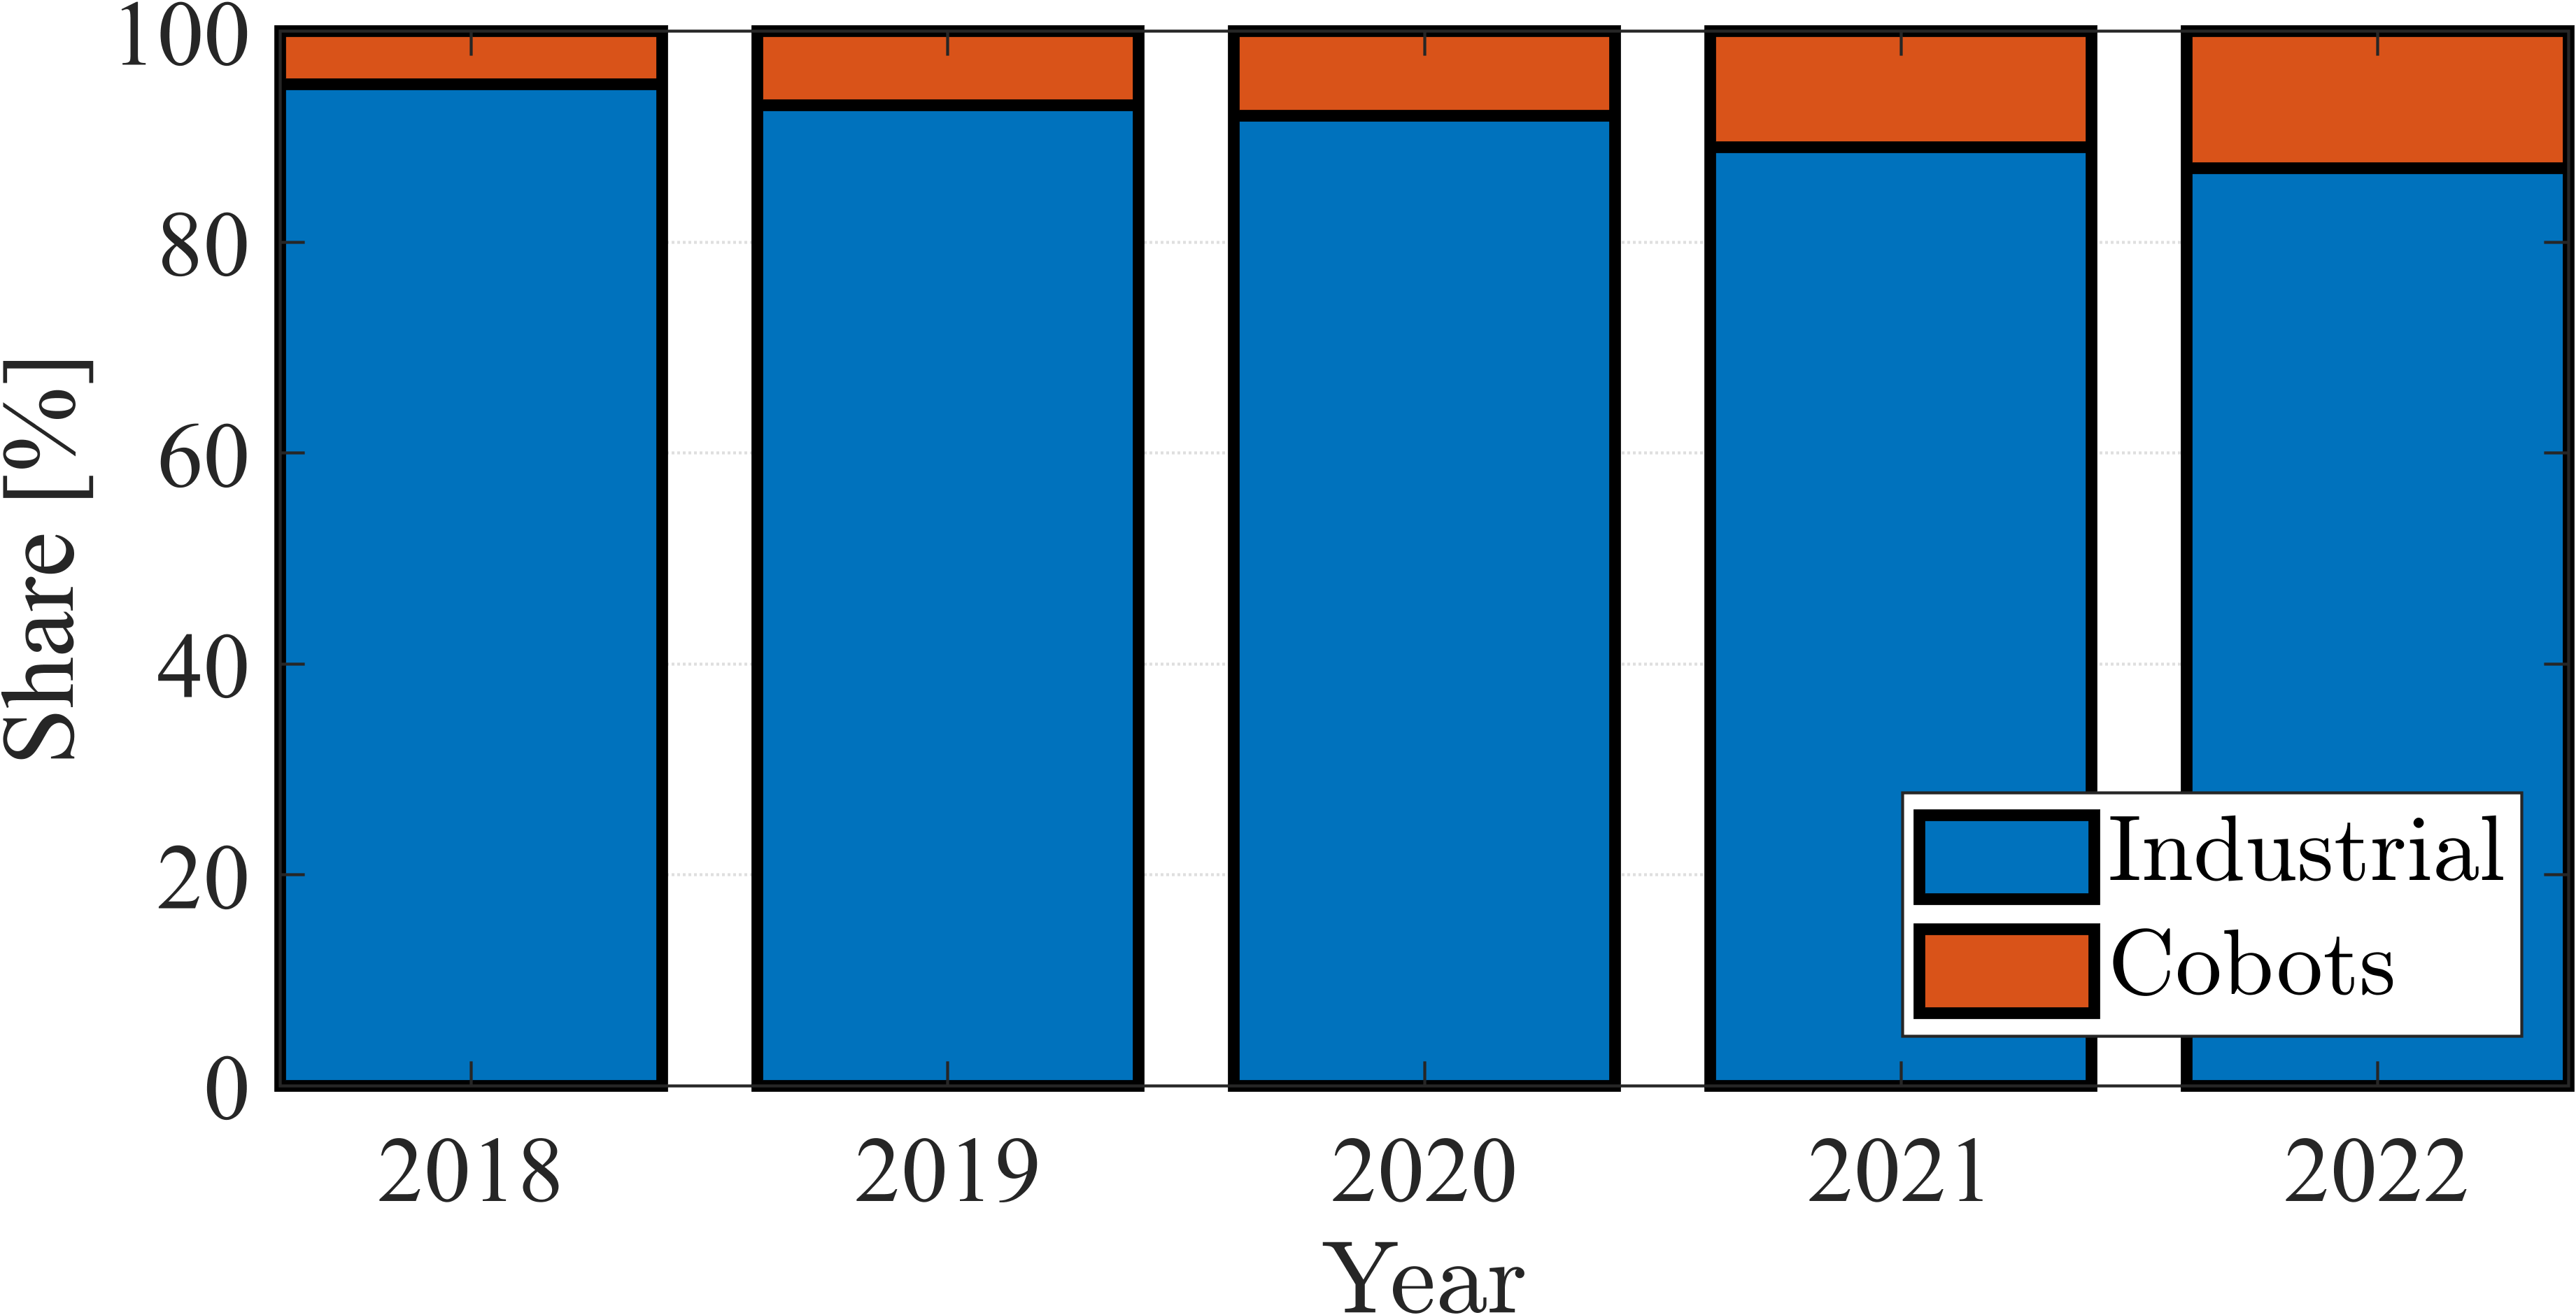
\includegraphics[width= 0.45\textwidth]{fig/share_industrial_and_cobots.png} 
	\caption{Unit sales share industrial robots to cobots }
	\label{fig:industrial_cobot_share}
\end{figure}
% ---

The unit sales are congruent with the the estimated operational stock of industrial (Fig.~\ref{fig:ir_stock}) robots and cobots (\ref{fig:cobot_stock}).
% ---
\begin{figure*}[!h]
	\centering
	\hspace*{\fill}
	\begin{subfigure}[t]{0.45\textwidth}
		\subcaption{}
		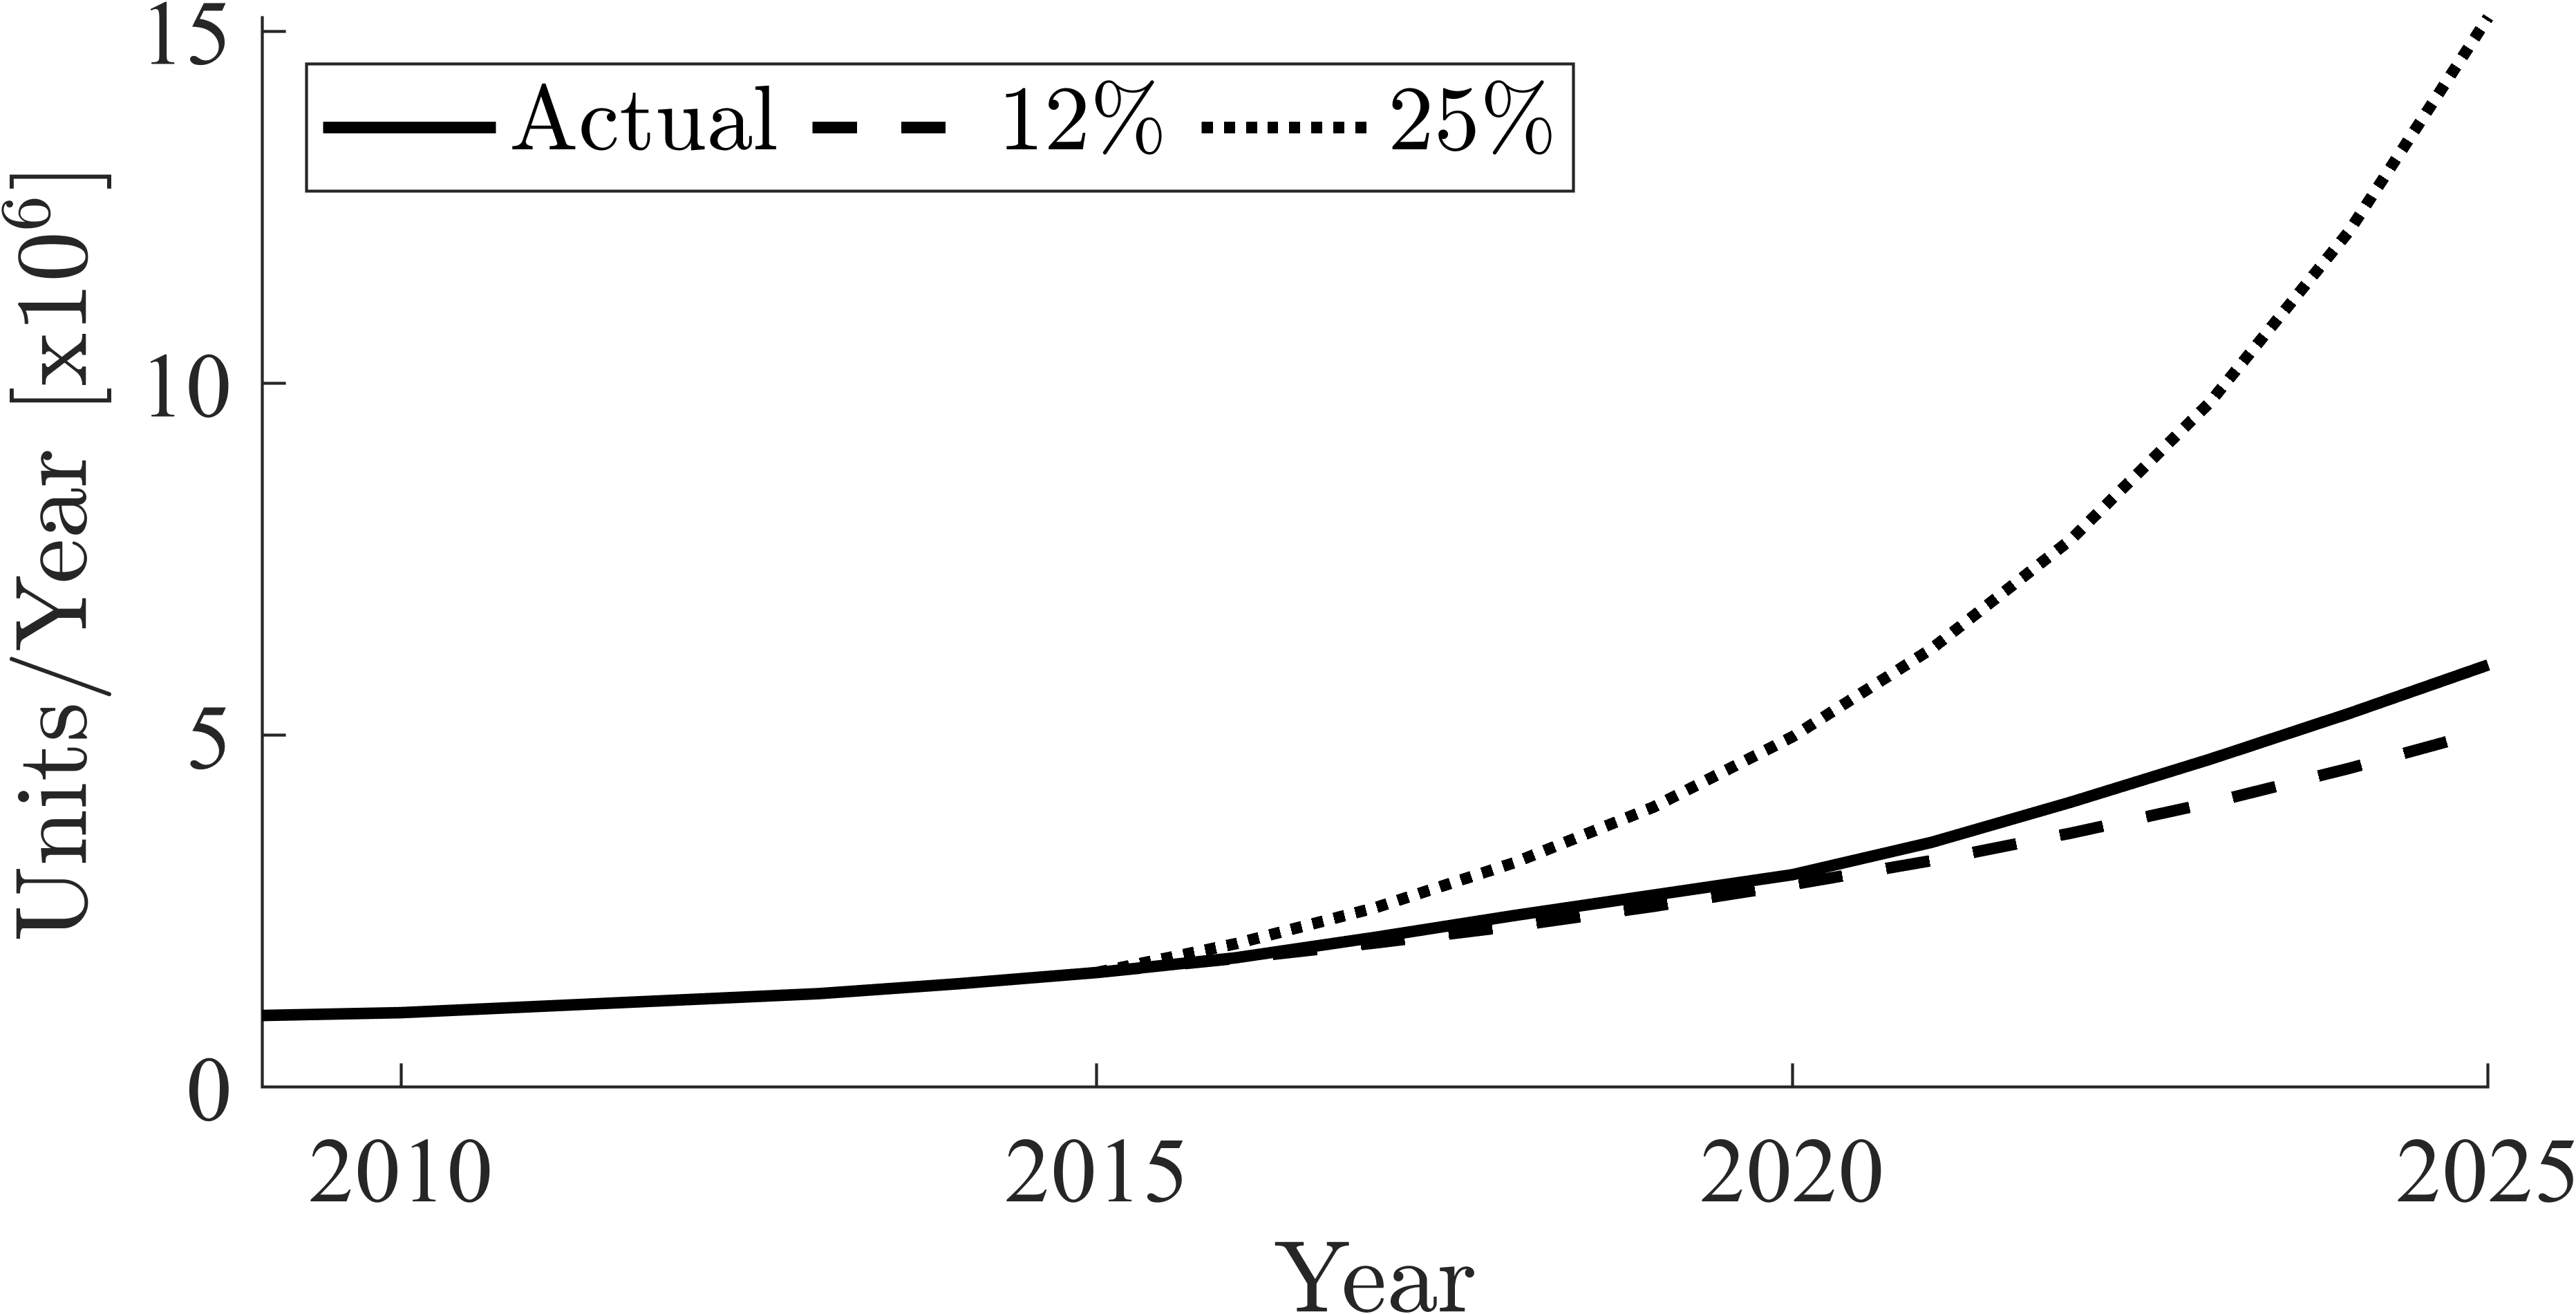
\includegraphics[width= \textwidth]{ir_units_projections.png}
		\label{fig:ir_stock}
	\end{subfigure}
	\hfill
	\begin{subfigure}[t]{0.45\textwidth}
		\subcaption{}
		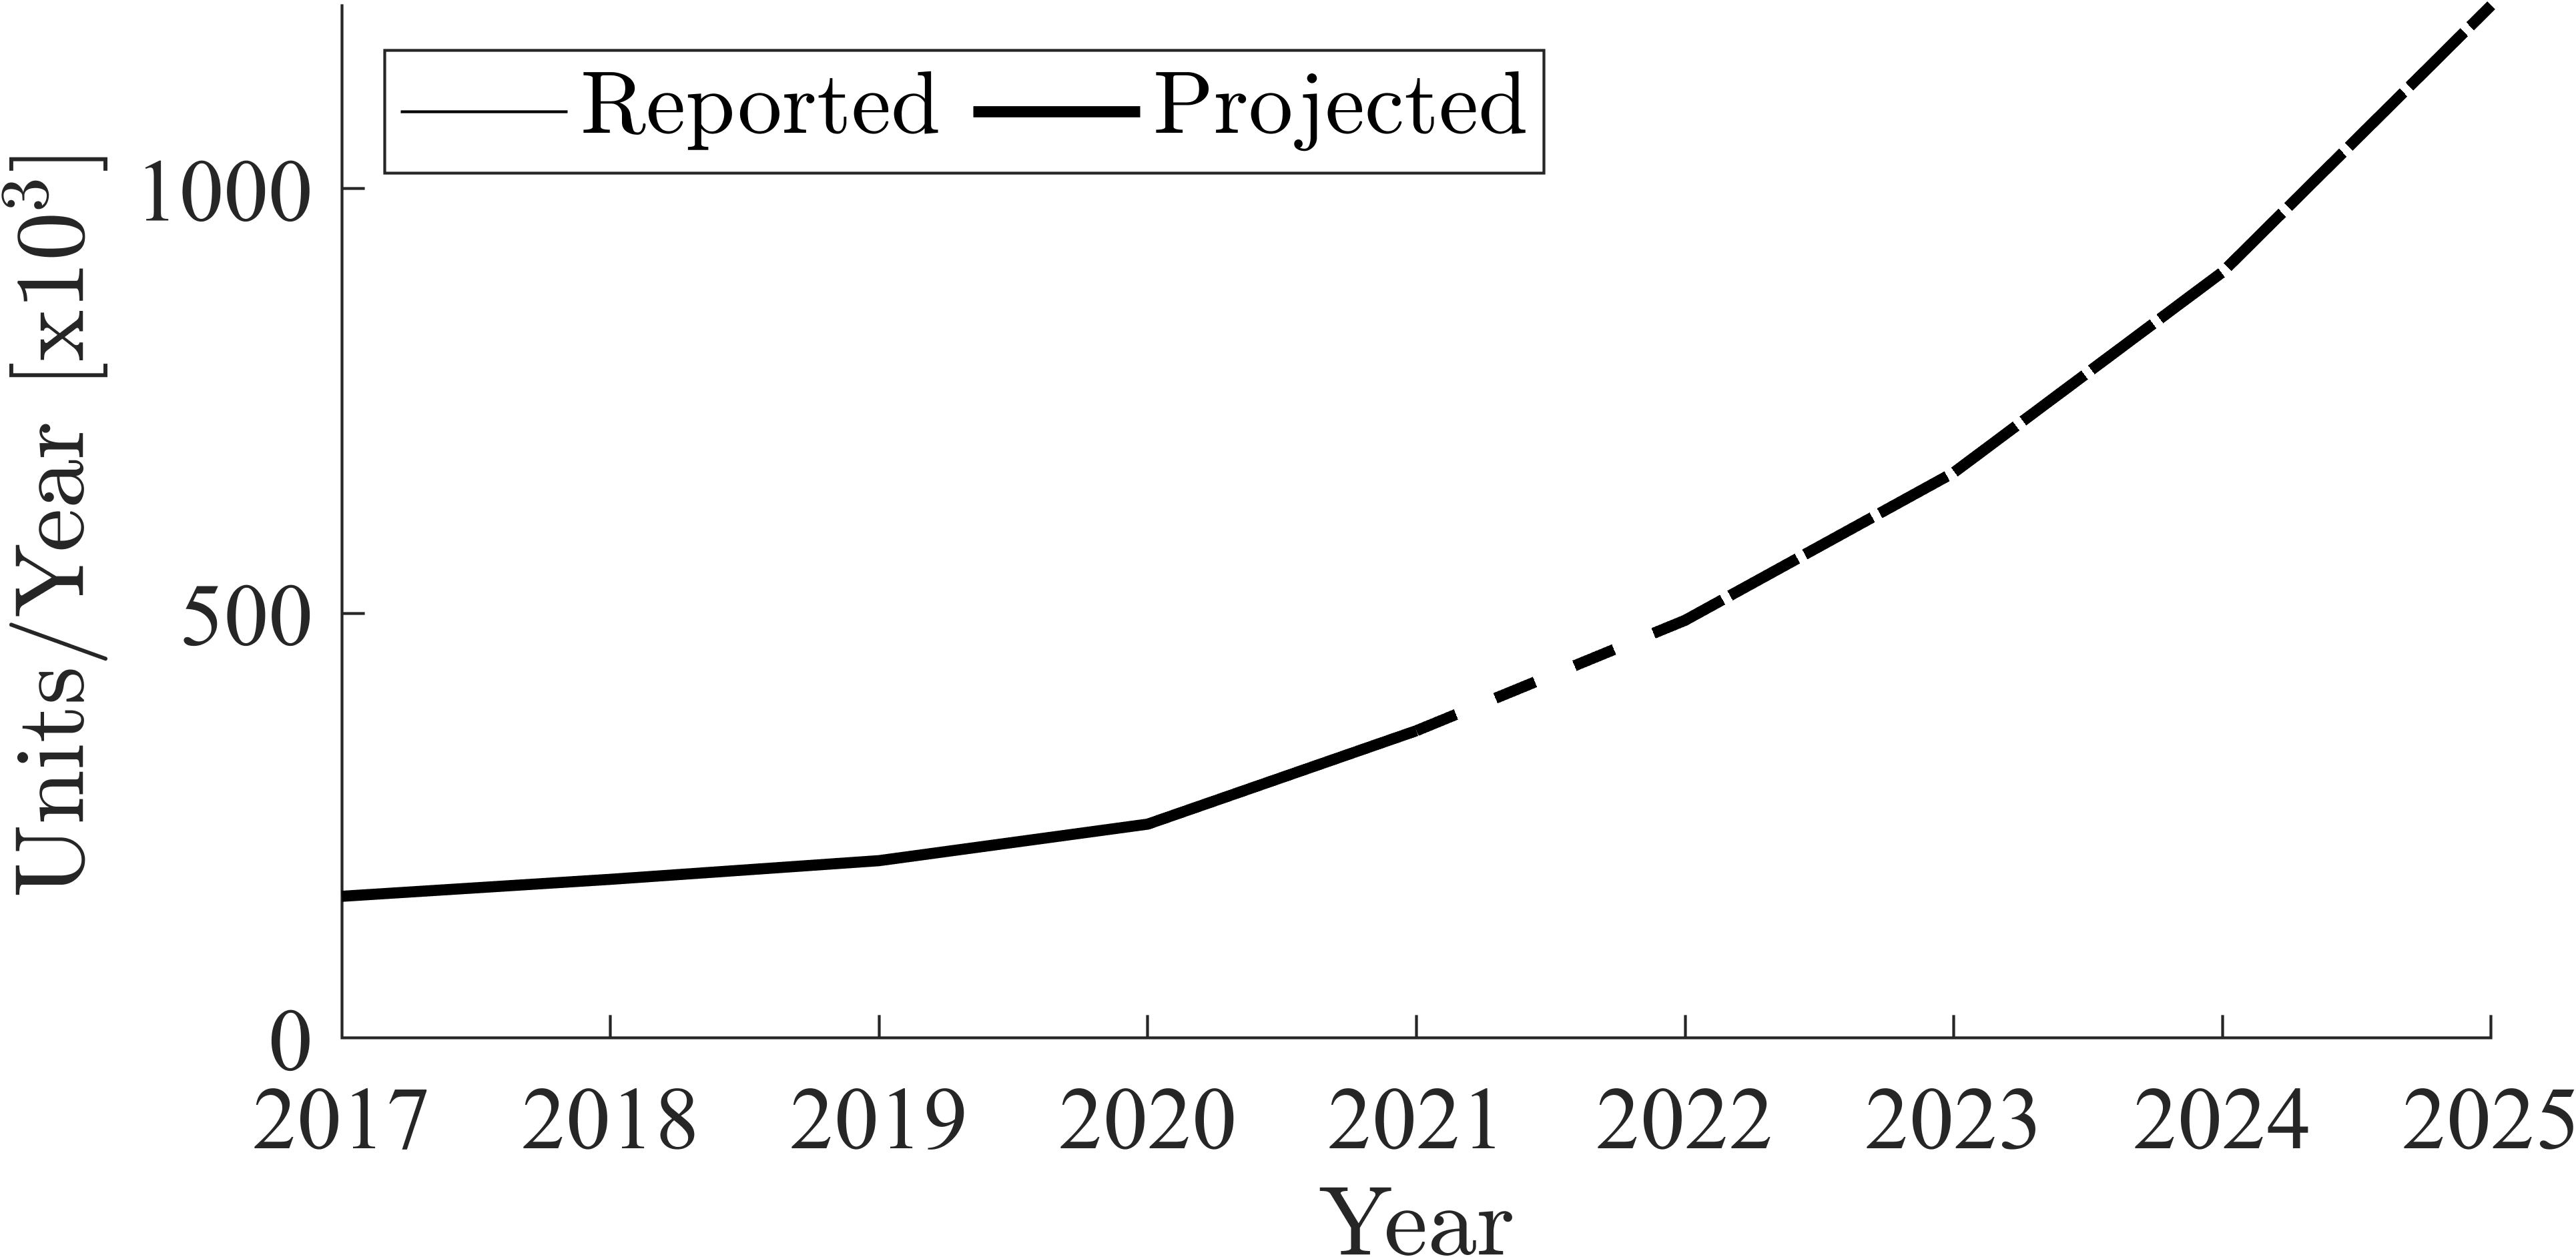
\includegraphics[width= \textwidth]{cb_units_projections.png}
		\label{fig:cobot_stock}
	\end{subfigure}
	\hspace*{\fill}	
	\caption[] {\label{fig:robot_forecasts} Forecasts for robot operational stock. \subref{fig:ir_stock} industrial robots install base forecast and \subref{fig:cobot_stock} cobots install base forecast.}	
\end{figure*}
% ===================================================================================================
%                                                 |                                                 |
%                                                 |                                                 |
% -------------------------------------------- SECTION ---------------------------------------------|
%                                                 |                                                 |
%                                                 |                                                 |
% ===================================================================================================
\newpage
\section{Industrial robot energy consumption support data}\label{sec:app_robot_ener_consumption}
To provide estimates of the worldwide energy consumption of industrial and collaborative robots we surveyed various sources including reports from consulting agencies and non-profit organizations, news articles and manufacturer press releases and data-sheets to determine essential data such as the operational stock and power consumption per type of robot.

\subsection{Industrial robots}
According to \cite{montaqim2015} and available press releases of different robotic companies \cite{fanuc2015, yaskawa2014, ABB2015}, the approximate distribution of the industrial robot install base per manufacturer is shown in Fig.~\ref{fig:manufacturers_pie}.
% ---
\begin{figure*}[!h]
	\centering
	\hspace*{\fill}
	\begin{subfigure}[t]{0.45\textwidth}
		\subcaption{}
		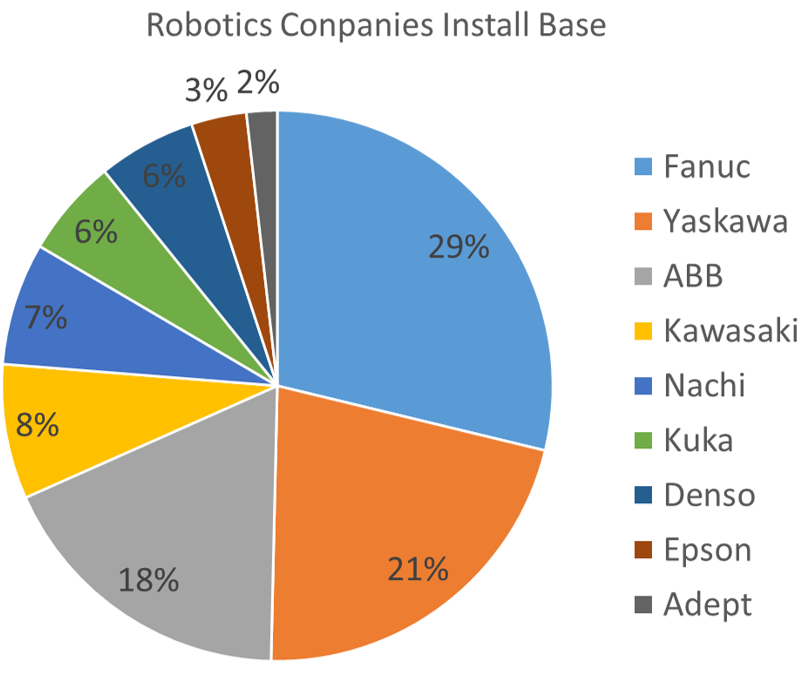
\includegraphics[width= \textwidth]{manufacturers}
		\label{fig:manufacturers_pie}
	\end{subfigure}
	\hfill
	\begin{subfigure}[t]{0.45\textwidth}
		\subcaption{}
		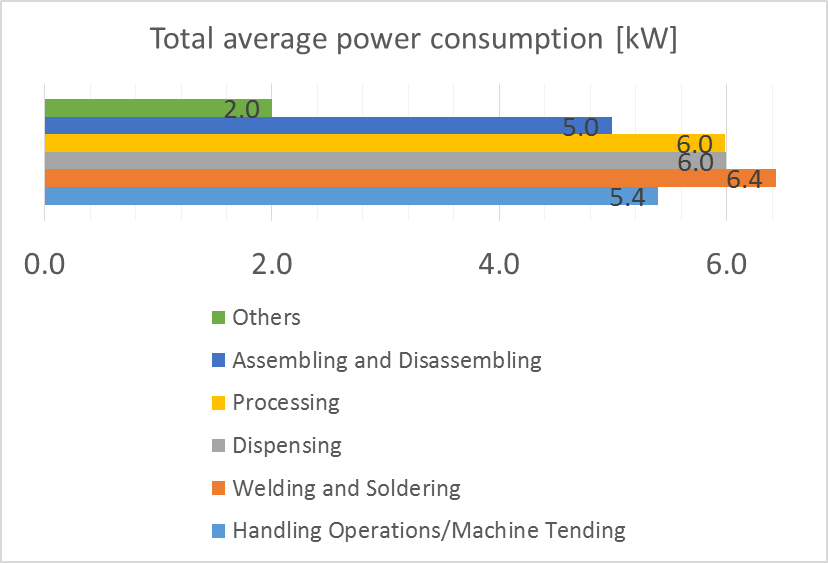
\includegraphics[width=\textwidth]{industrial_robots_average_power_per_category} \label{fig:ir_average_power}
	\end{subfigure}
	\hspace*{\fill}
	\caption[] {\label{fig:ir_statistics} Industrial robots statistics. \subref{fig:manufacturers_pie} Percentage of installed industrial robots per manufacturer and \subref{fig:ir_average_power} average power consumption of industrial robots per category.}
\end{figure*}
% ---

Since Fanuc, Yaskawa, and ABB make for two-thirds of the total install base of industrial robots, we took the power consumption of the robots from those manufacturers to estimate the total power consumption. After surveying the data-sheets for the different robot types in their portfolio, the average power consumption for each model was estimated. Additionally, every manufacturer classifies their robots according to one or more possible applications, which can be grouped into the application categories defined by the IFR. The average power consumption was calculated for every application using the values reported in the robot data-sheets. Finally, the power consumption for each category was computed as a weighted average based on the companies' market share percentage (assuming that 68 \% is the total number of robots)\footnote[1]{These numbers should be used with discretion since there is no available information on which are the most common installed robot models. This information may change the estimation.}. The estimated power consumption per robot application is shown in Fig.~\ref{fig:ir_average_power}. Using these numbers and the estimated operational stock of industrial robots reported in \cite{statista_ir_operational_stock} and by the International Federation of Robotics (see Fig.~\ref{fig:ir_stock}), the estimated worldwide industrial robot energy consumption was computed and shown in Fig.~\ref{fig:ir_energy}.

% ===================================================================================================
\subsection{Collaborative robots}\label{sec:app_cobot_ener_consumption}
%---
\begin{figure}[!h]
	\centering
	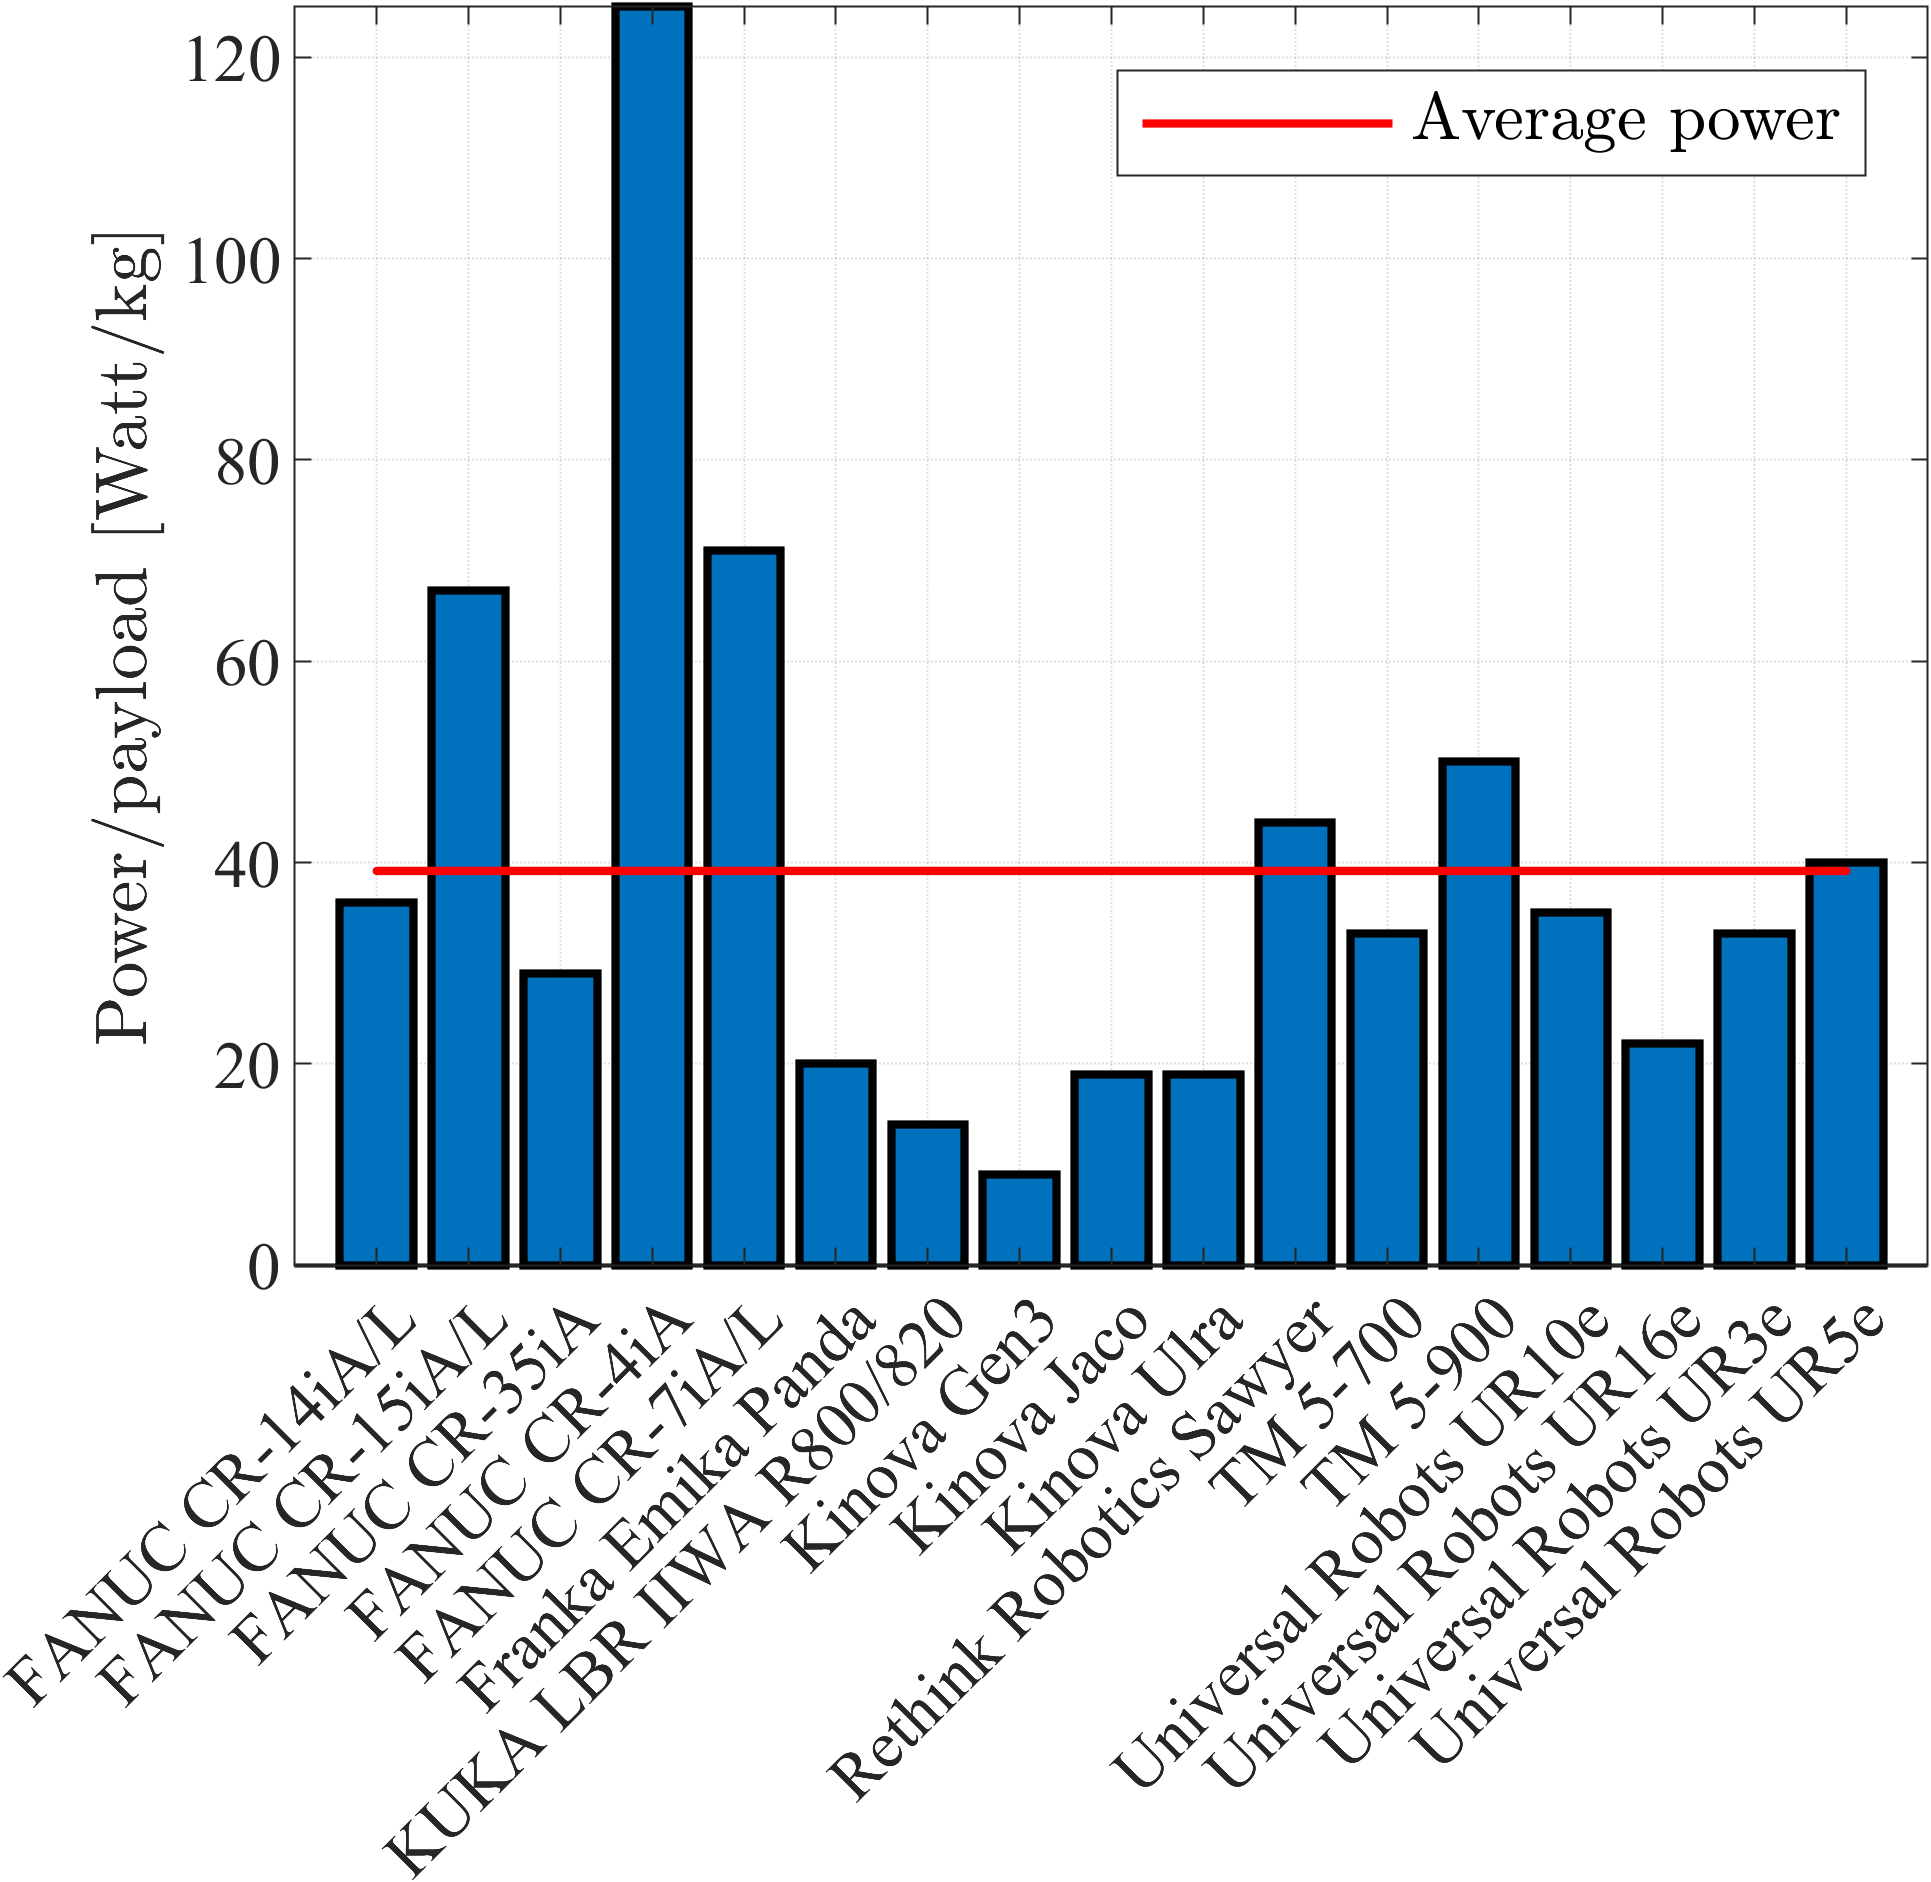
\includegraphics[width=0.45\textwidth]{cobot_watt_per_kg.png}
	\caption{Power consumption per payload for different cobots.}
	\label{fig:cobot_watt_per_kg}
\end{figure}
%---
To approximate the energy consumption of cobots we looked at the power consumption per payload of various manufacturers, see Fig.~\ref{fig:cobot_watt_per_kg} resulting in an average power consumption of approximately 40 W. Together with a typical power consumption of the robot controller of 60 W \cite{Heredia2023BreakingEnergyConsumption}, we consider a total of 100 W power demand. Similar to the industrial robots, the worldwide energy consumption was calculated assuming a 24/7 operation.





\end{document}